\chapter{Modèle SIR} \label{ch:intro}

\section{Mesures et méthodologie SIR}

Les mesures ainsi que les méthodologie sont les mêmes que pour le modèle SI, c'est-à-dire que les densité $\frac{1}{2},\frac{1}{4},\frac{1}{8},\frac{1}{16}$ et les tailles de populations $5000,20000,50000,100000$ sont étudiées.

\section{Résultats}

\begin{figure}[h]
	\centering
	\captionsetup{justification=centering}
	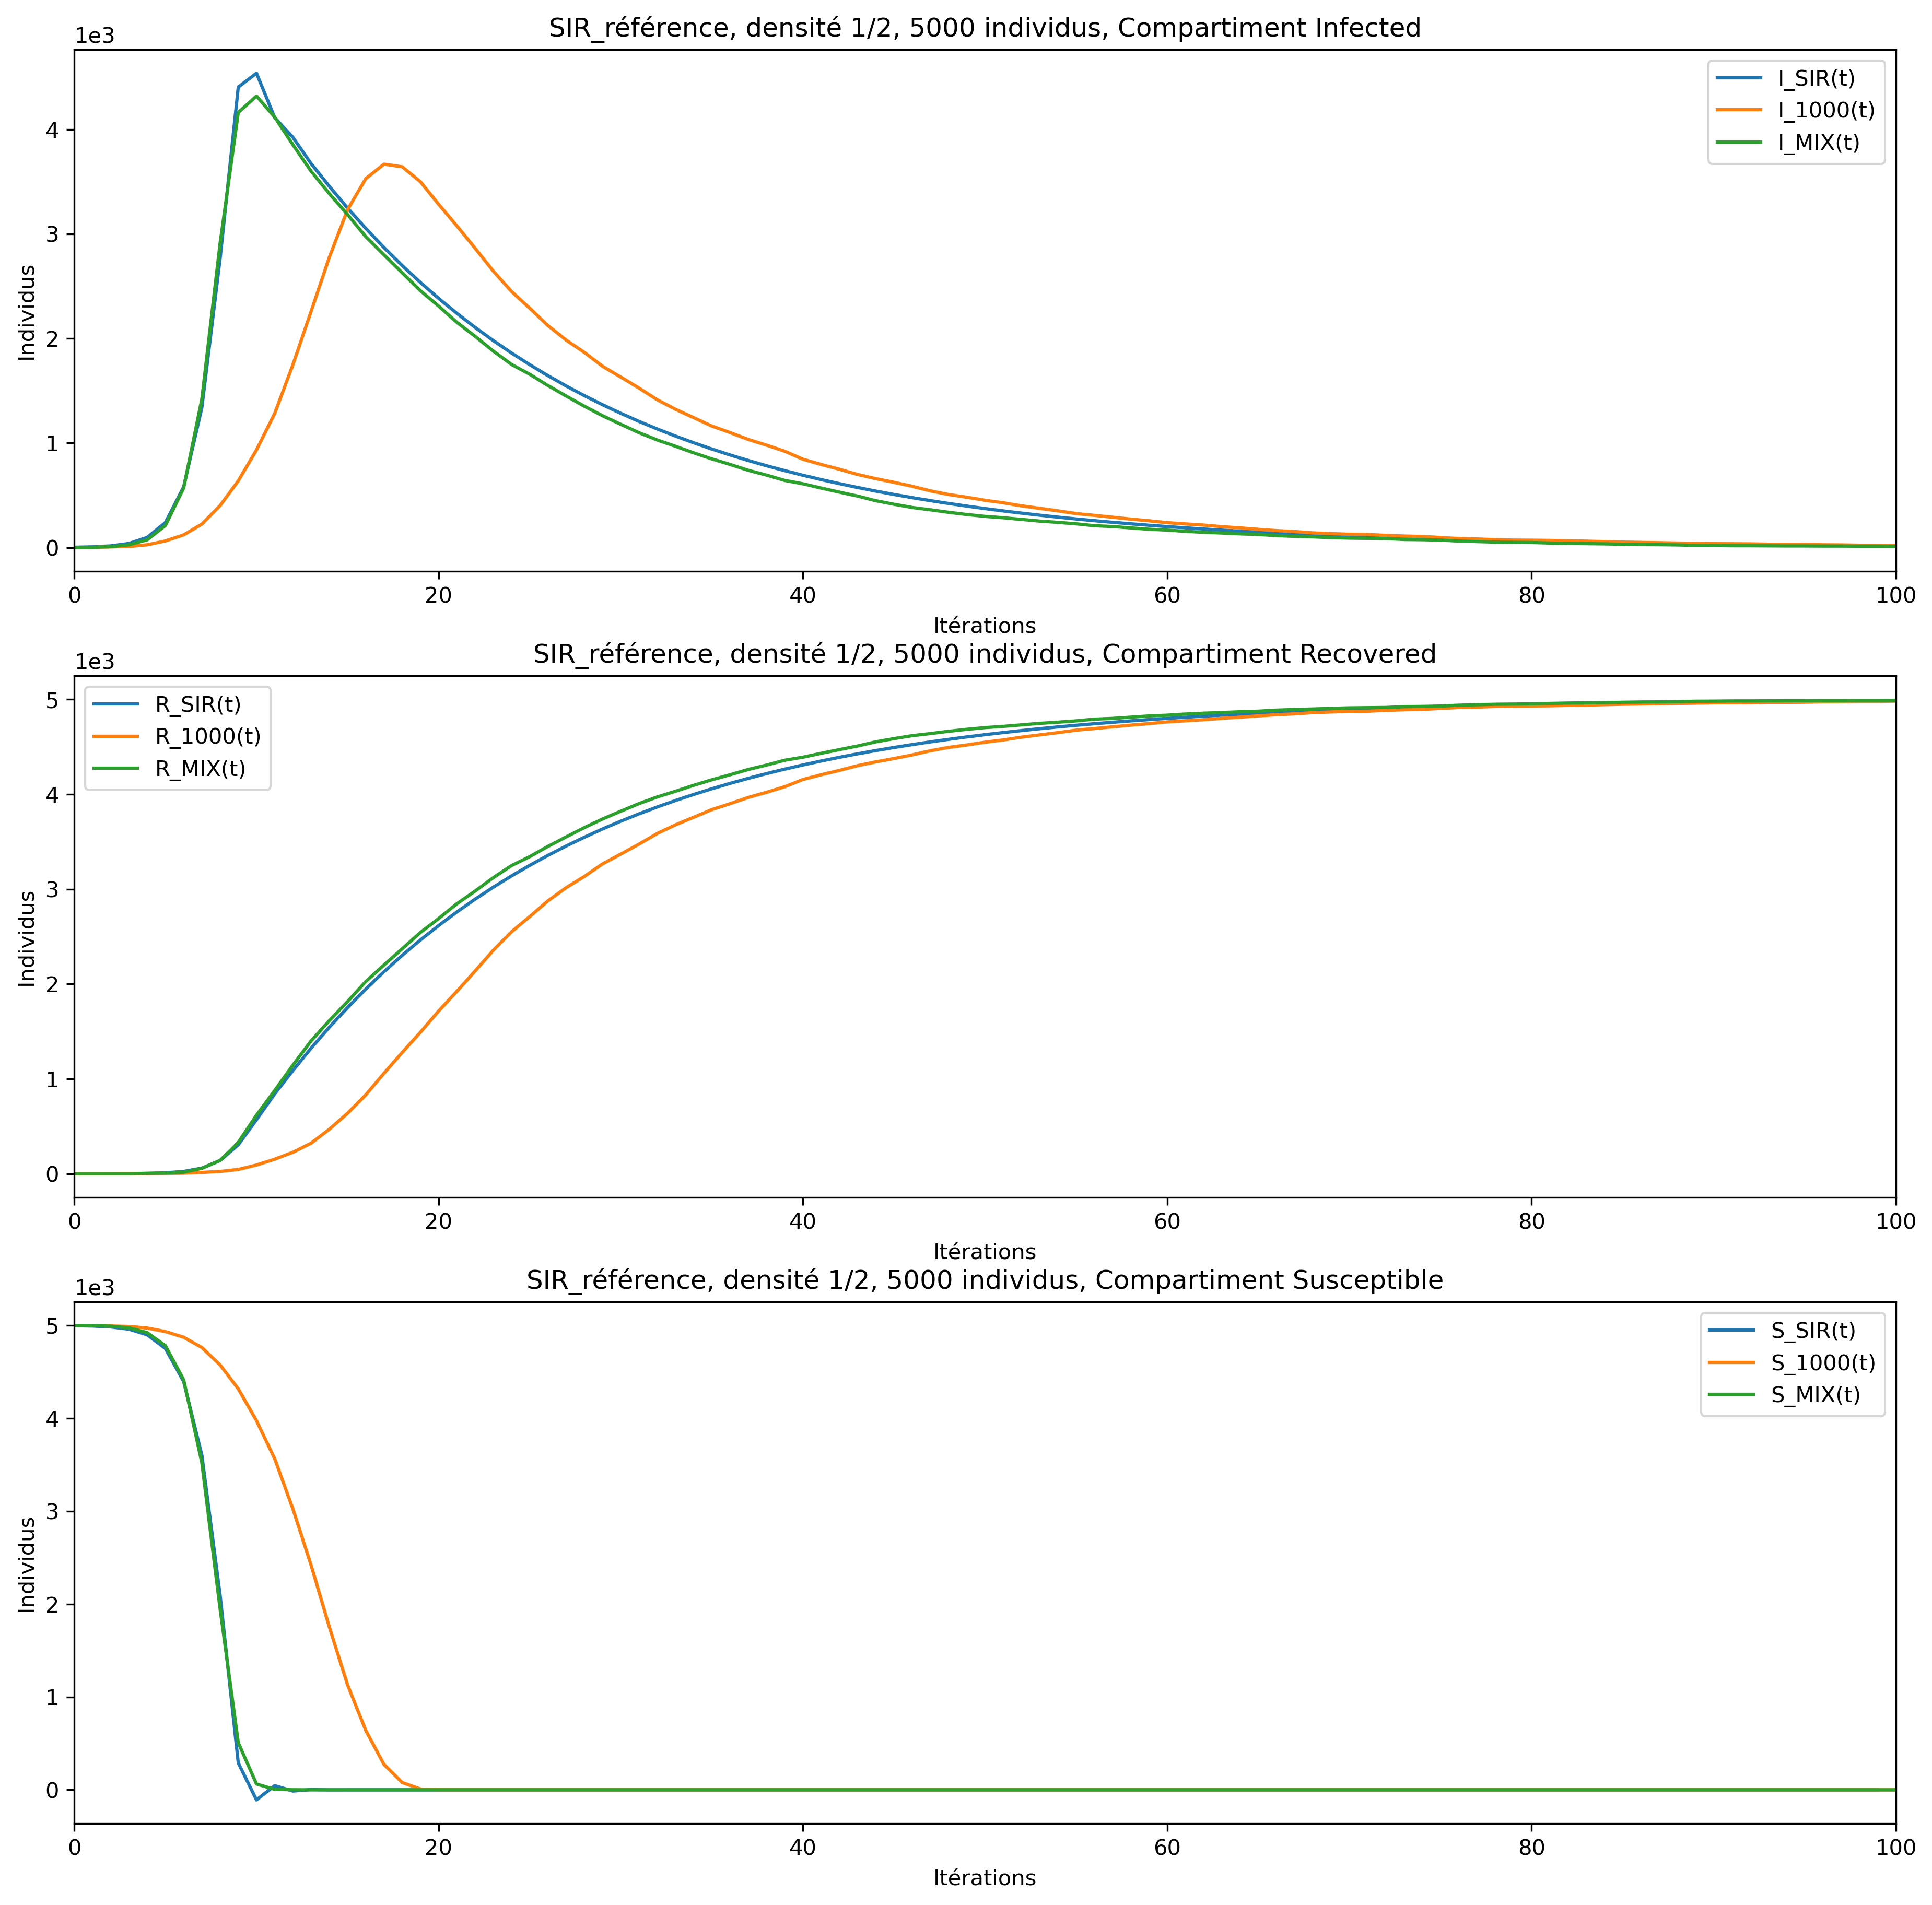
\includegraphics[width=.4\textwidth]{Images/SIR_ref_2_5.png}
	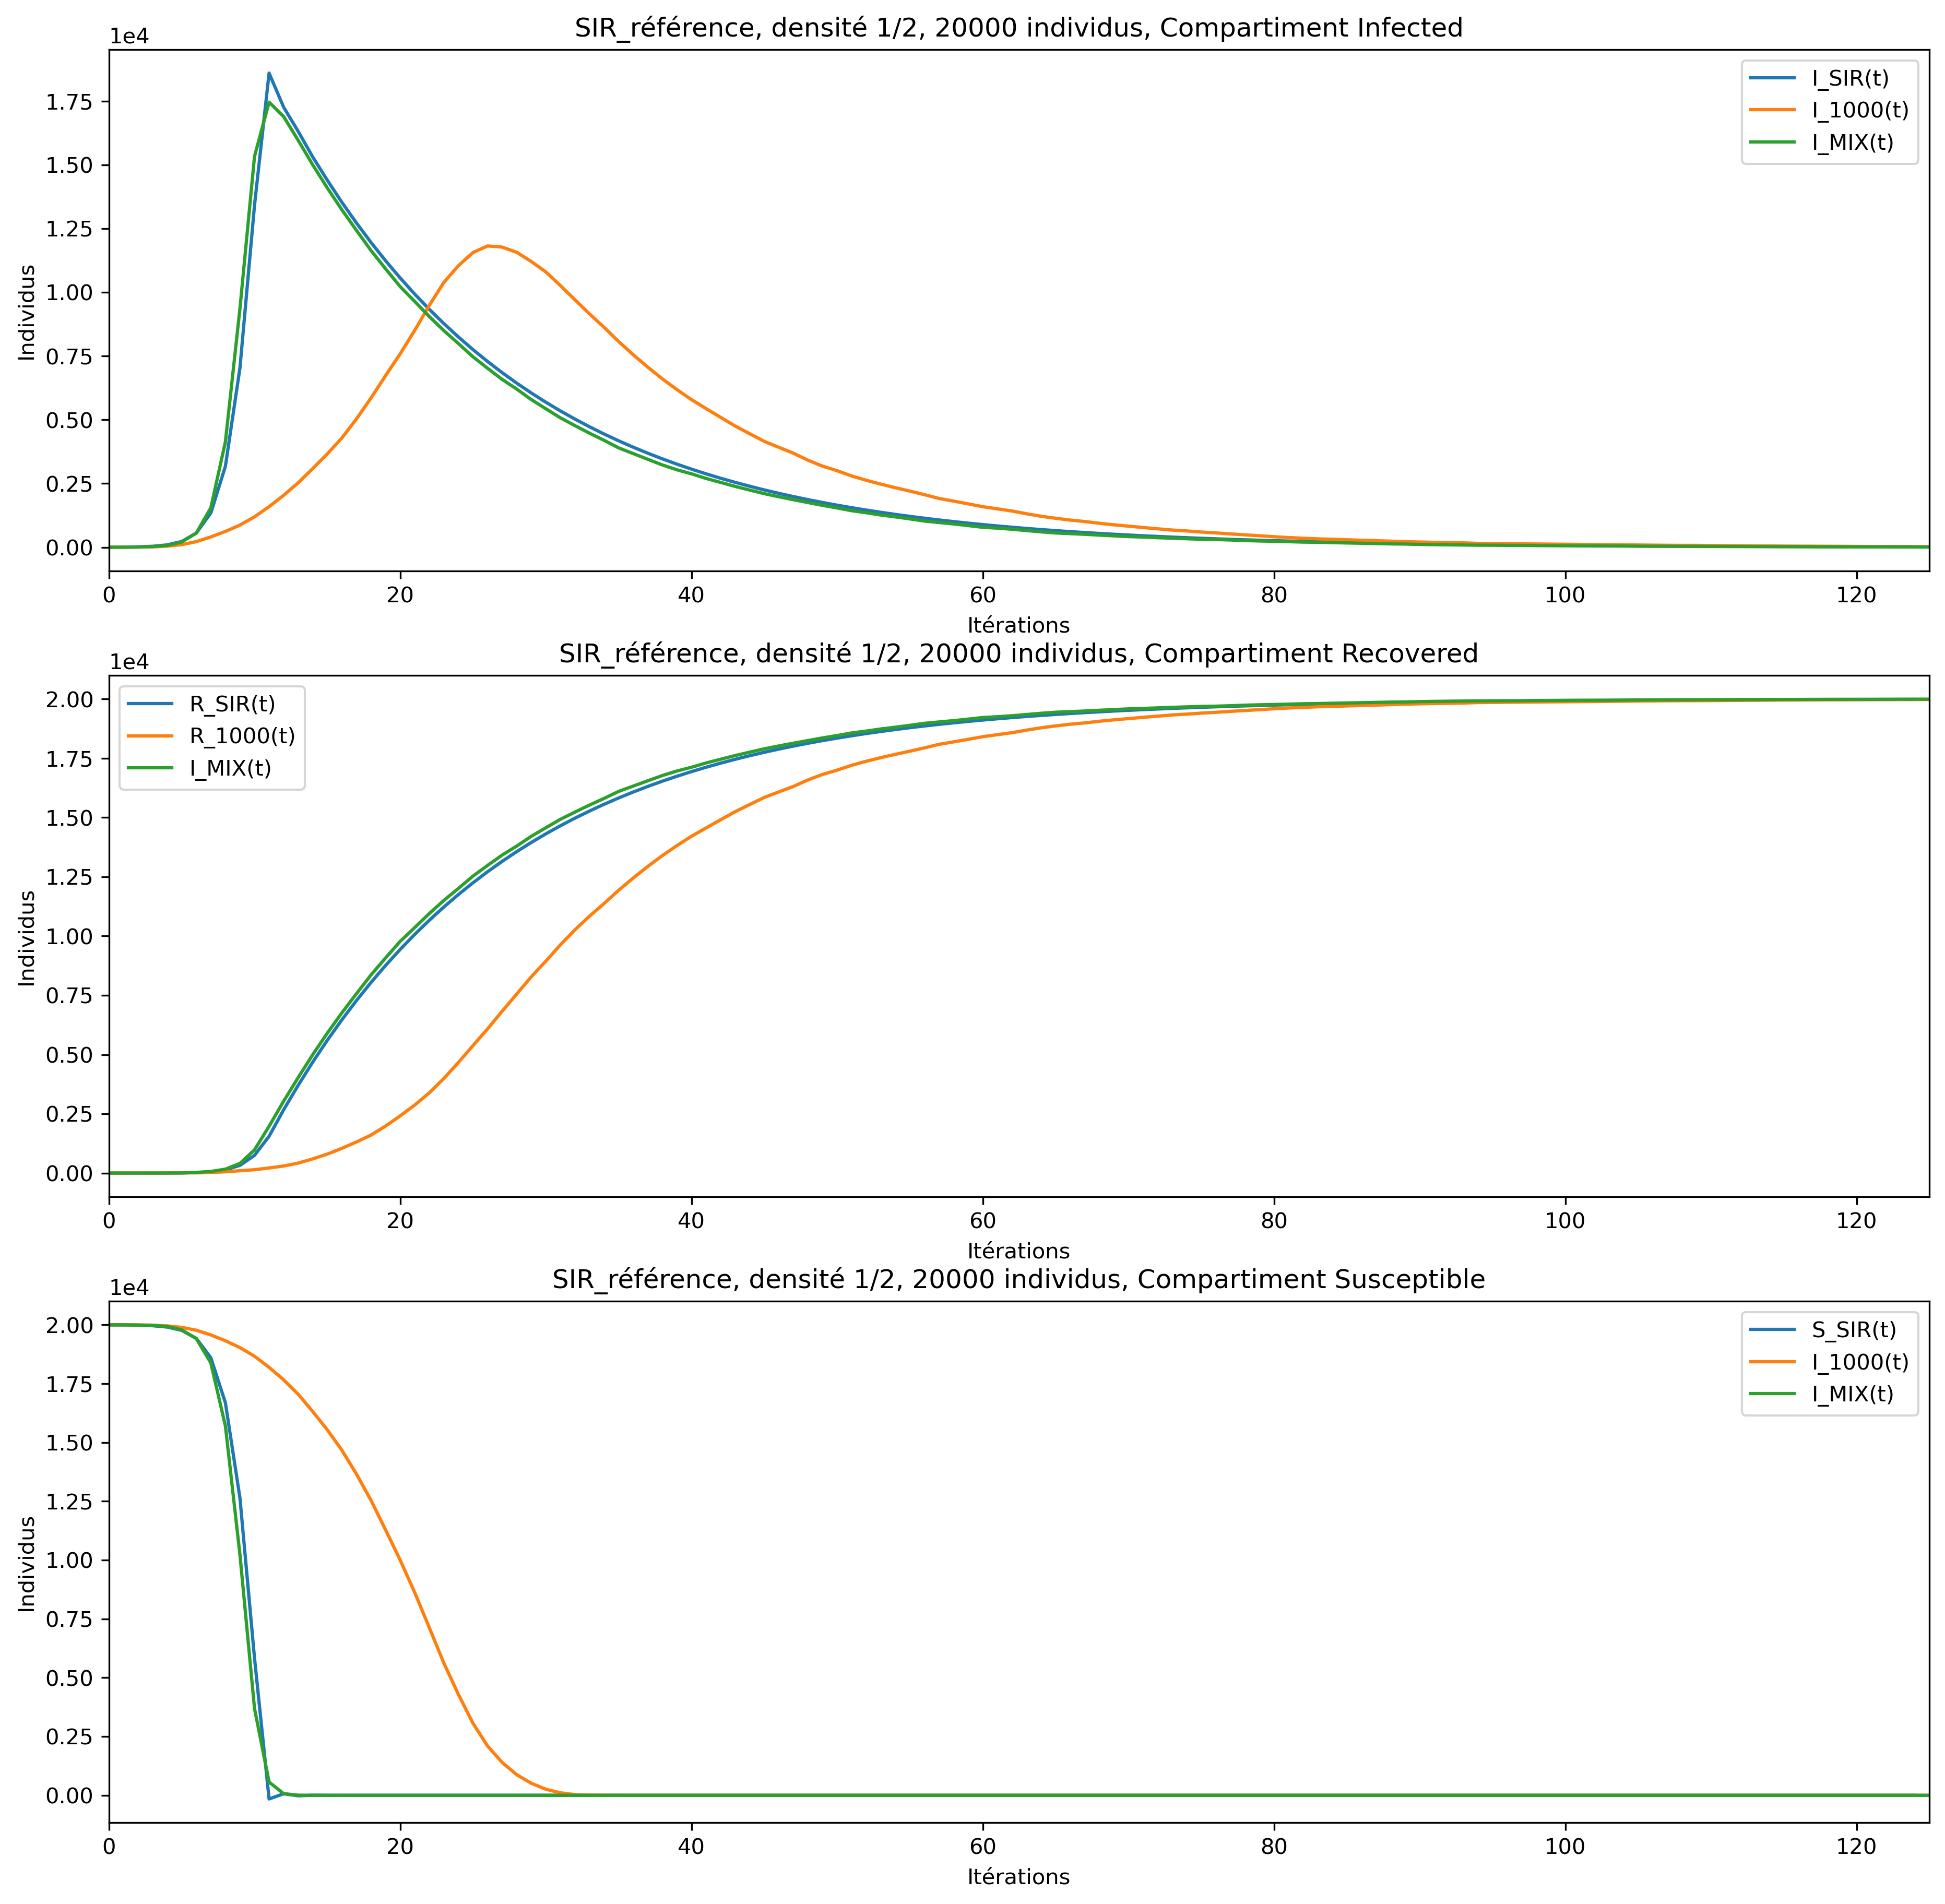
\includegraphics[width=.4\textwidth]{Images/SIR_ref_2_20.png}
	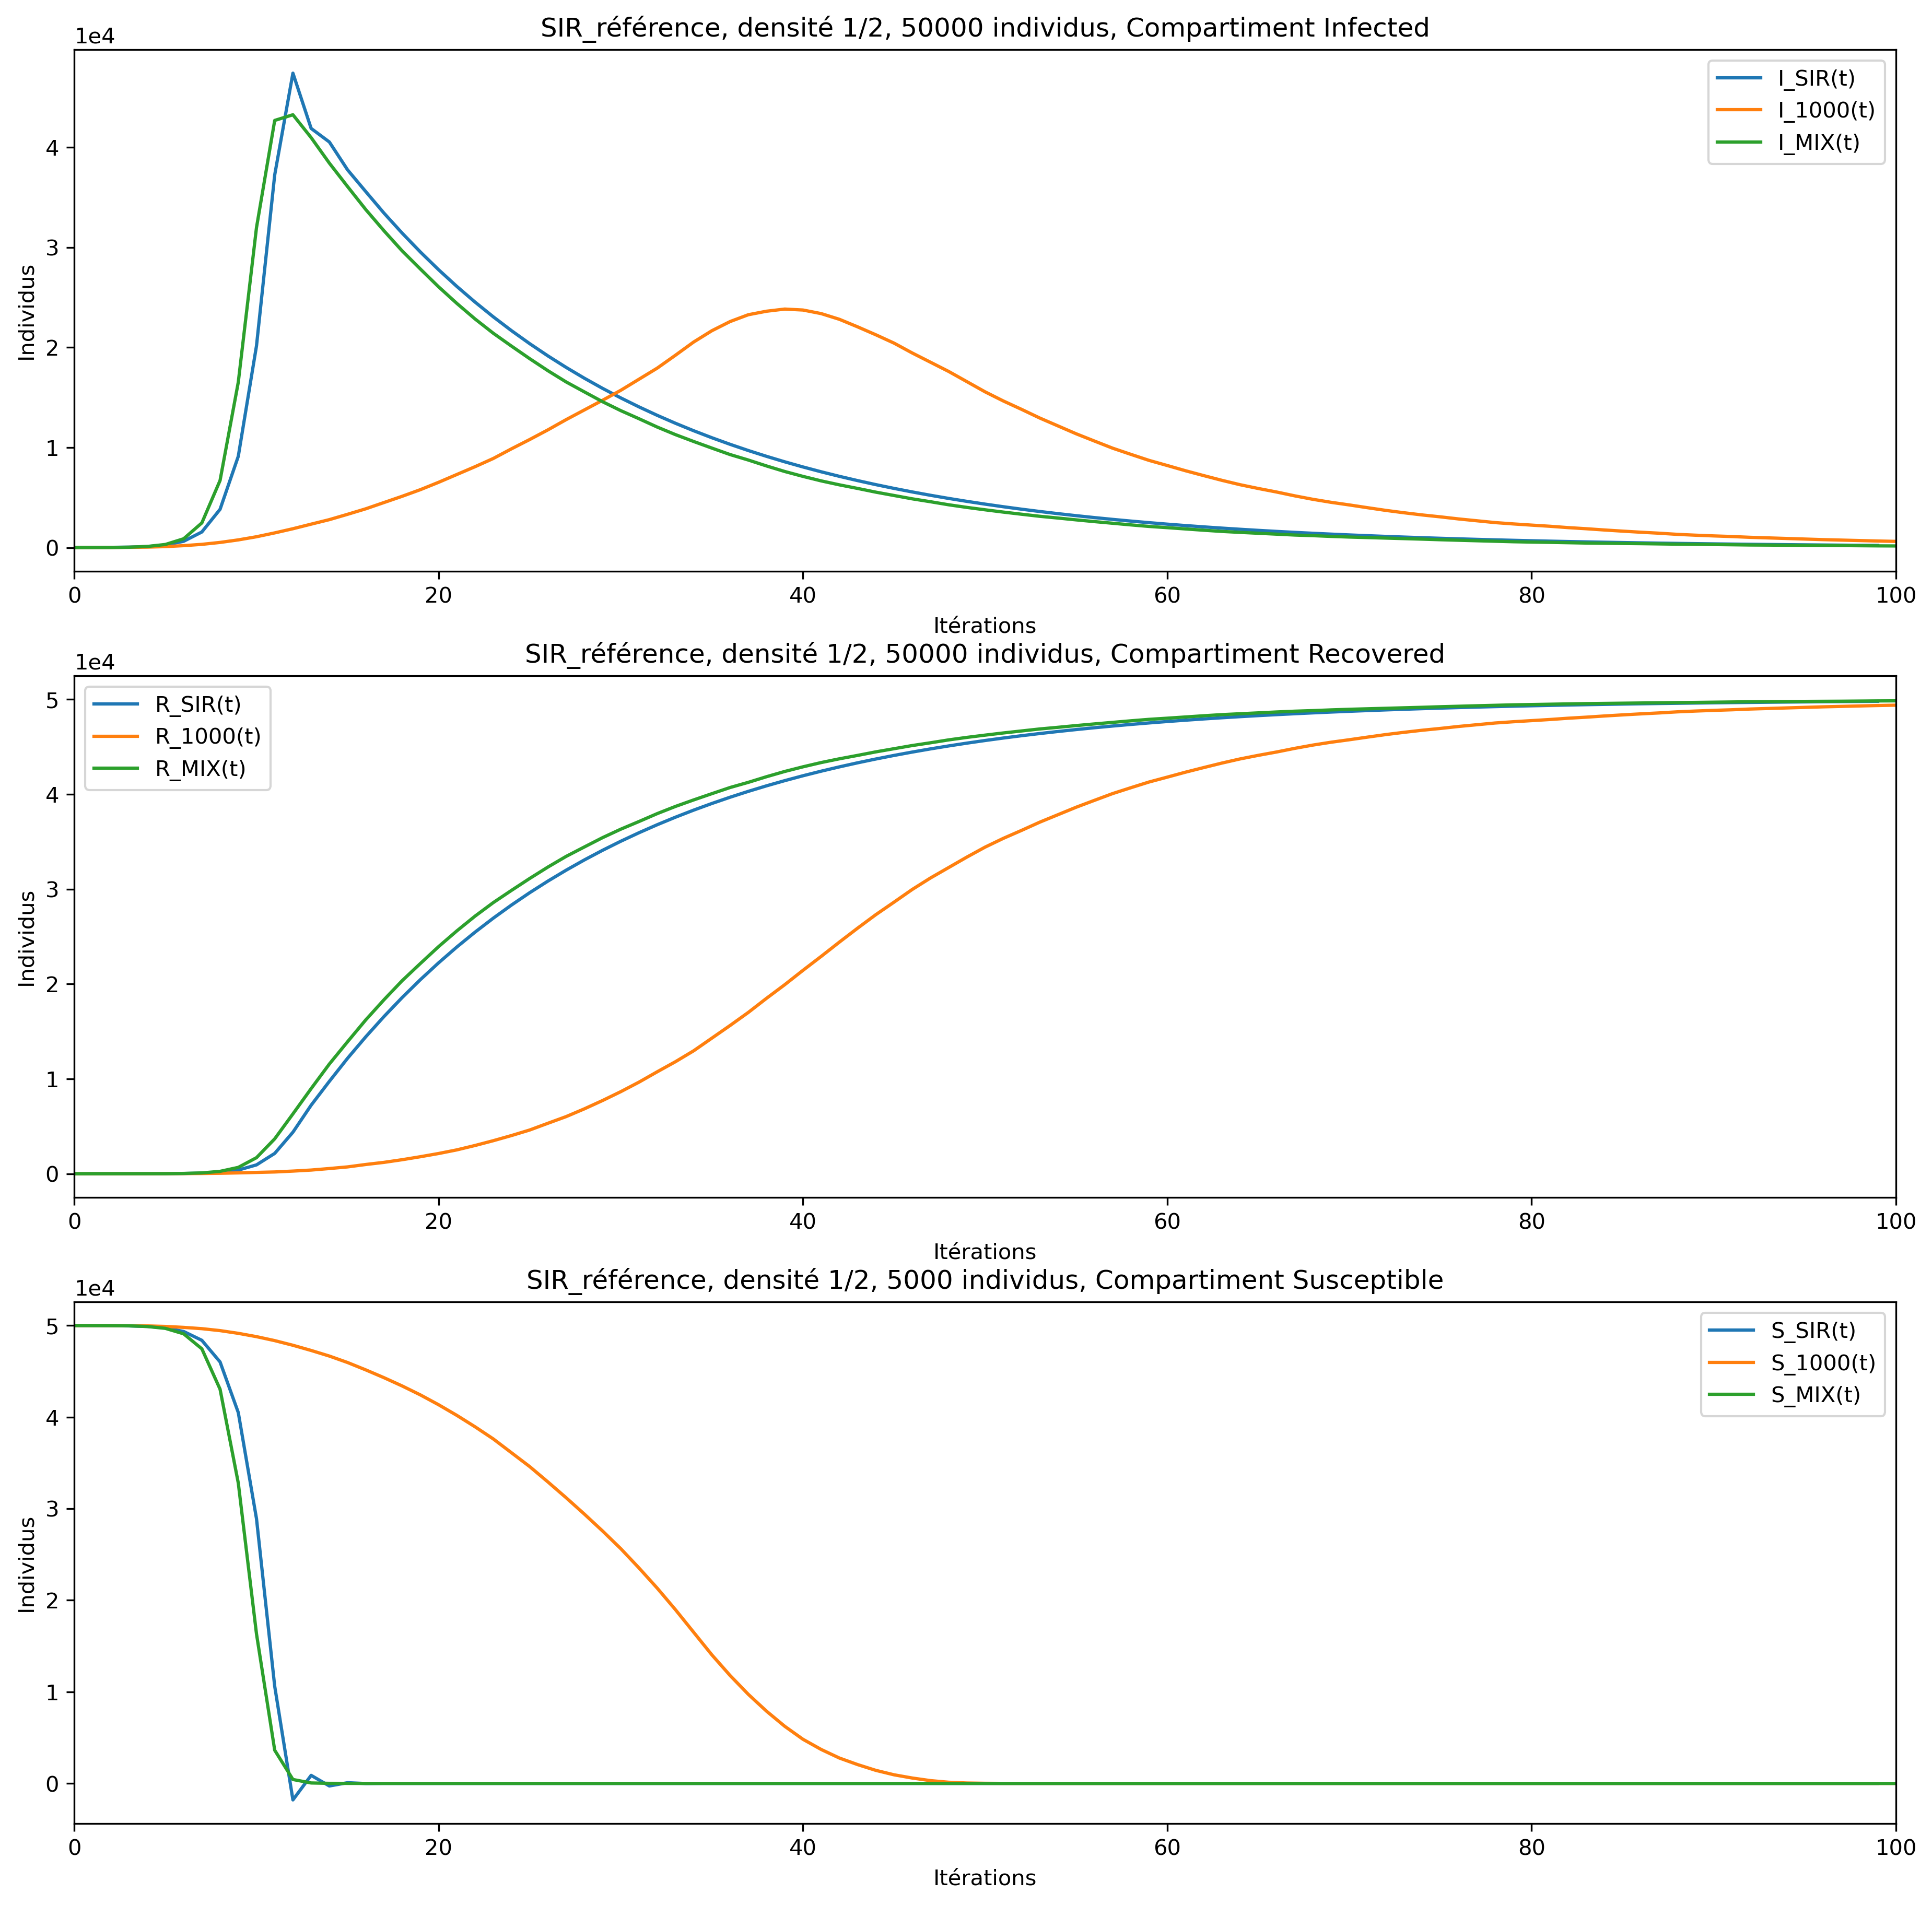
\includegraphics[width=.4\textwidth]{Images/SIR_ref_2_50.png}
	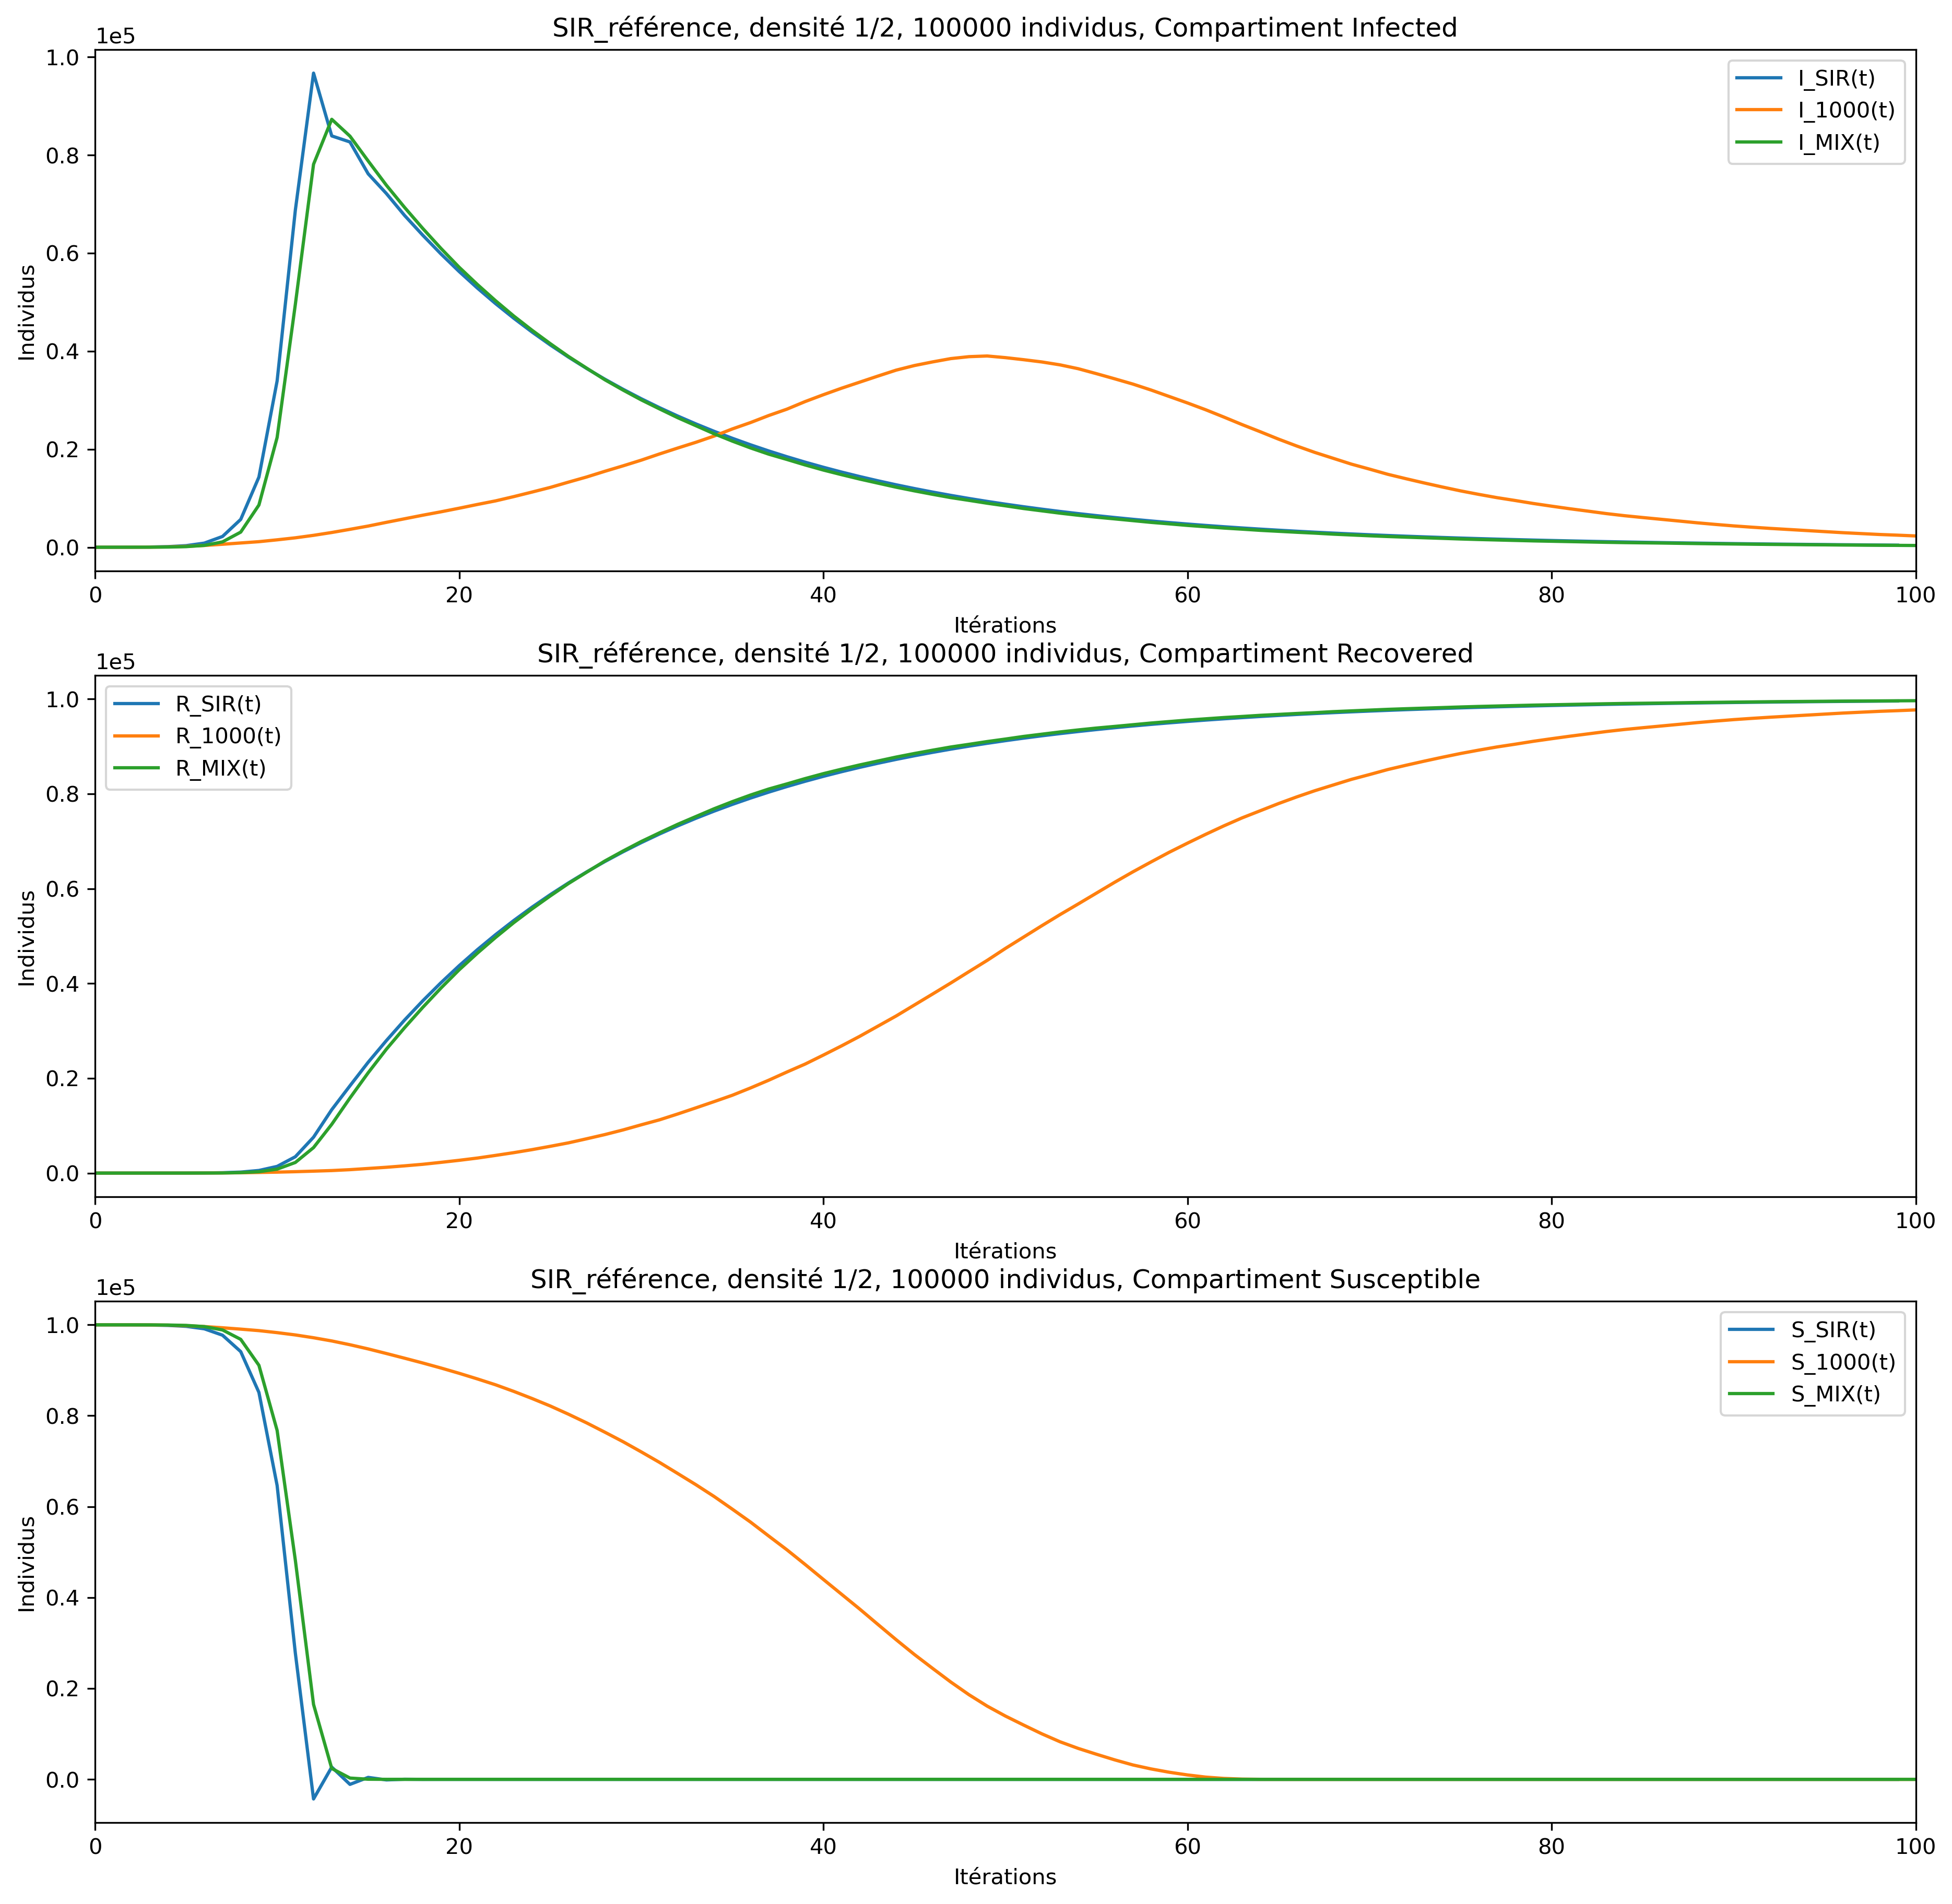
\includegraphics[width=.4\textwidth]{Images/SIR_ref_2_100.png}
	\caption{test}
\end{figure}

Pour les systèmes de forte densité, les simulations aux $1000$ mouvements peinent à se mélanger. Par conséquent, les événements sont plus tardifs. Nous pouvons observer les mêmes comportements que pour les simulations SI.

\newpage

\begin{figure}[h]
	\centering
	\captionsetup{justification=centering}
	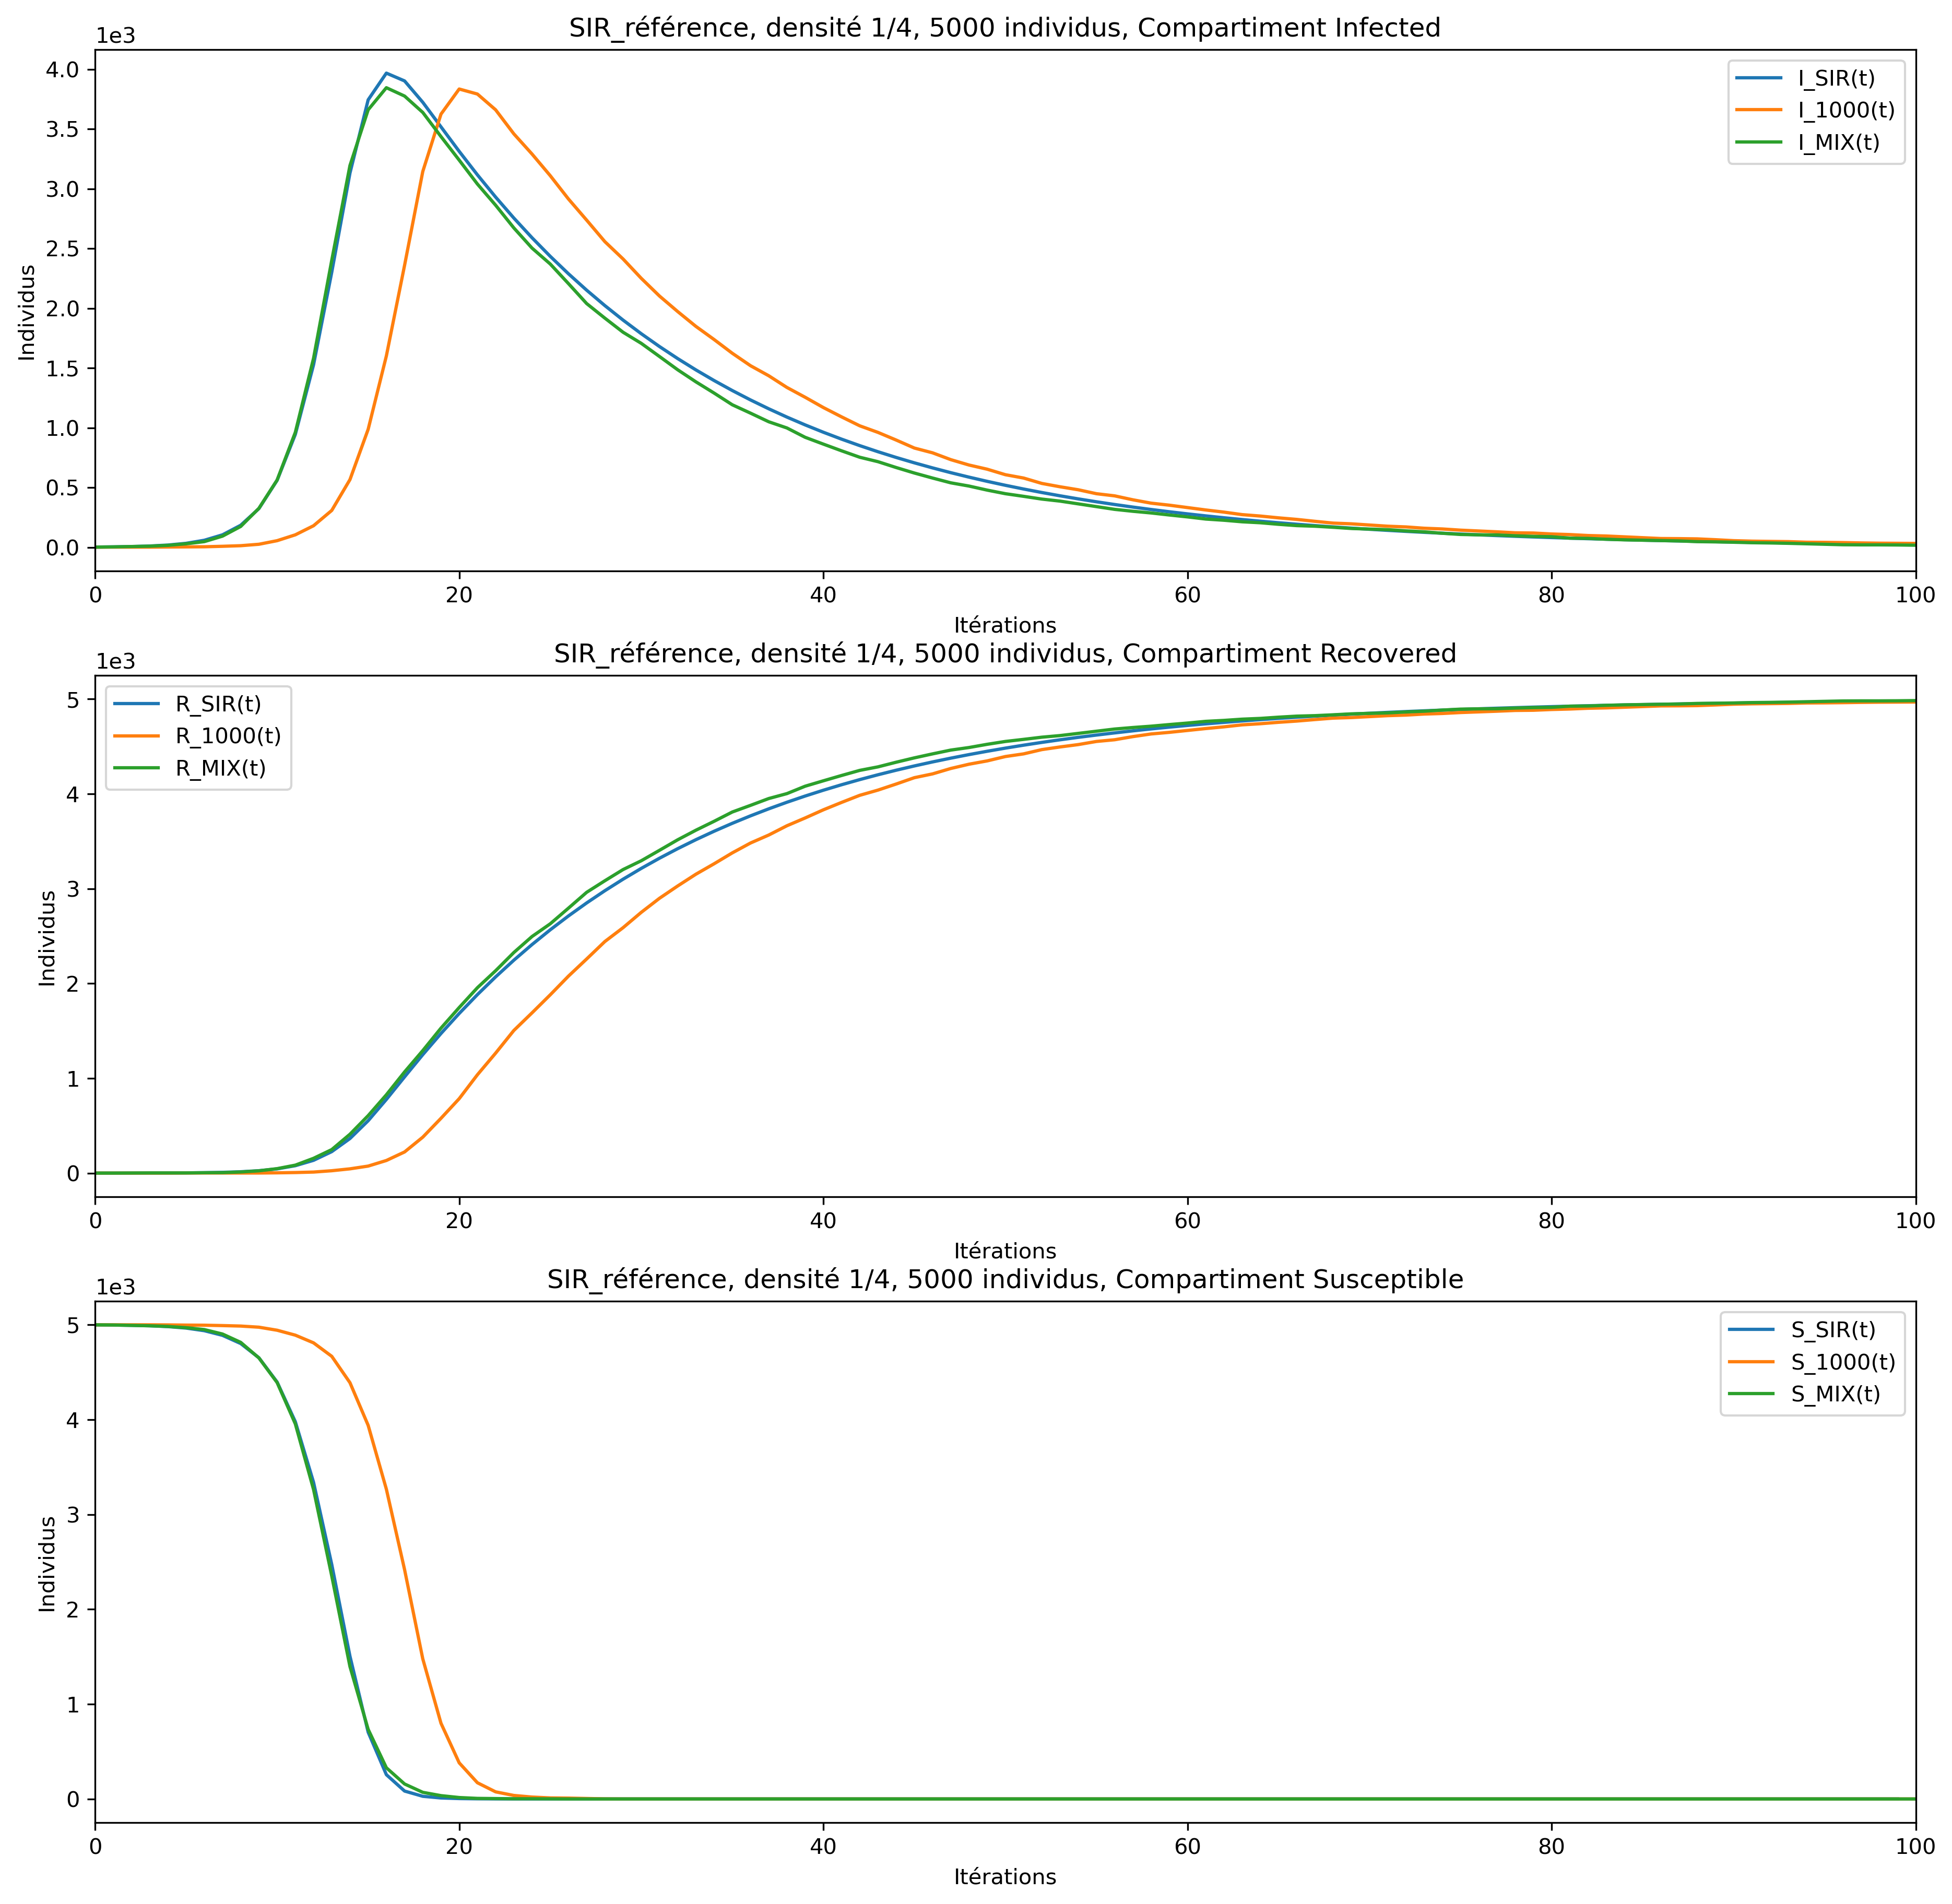
\includegraphics[width=.4\textwidth]{Images/SIR_ref_4_5.png}
	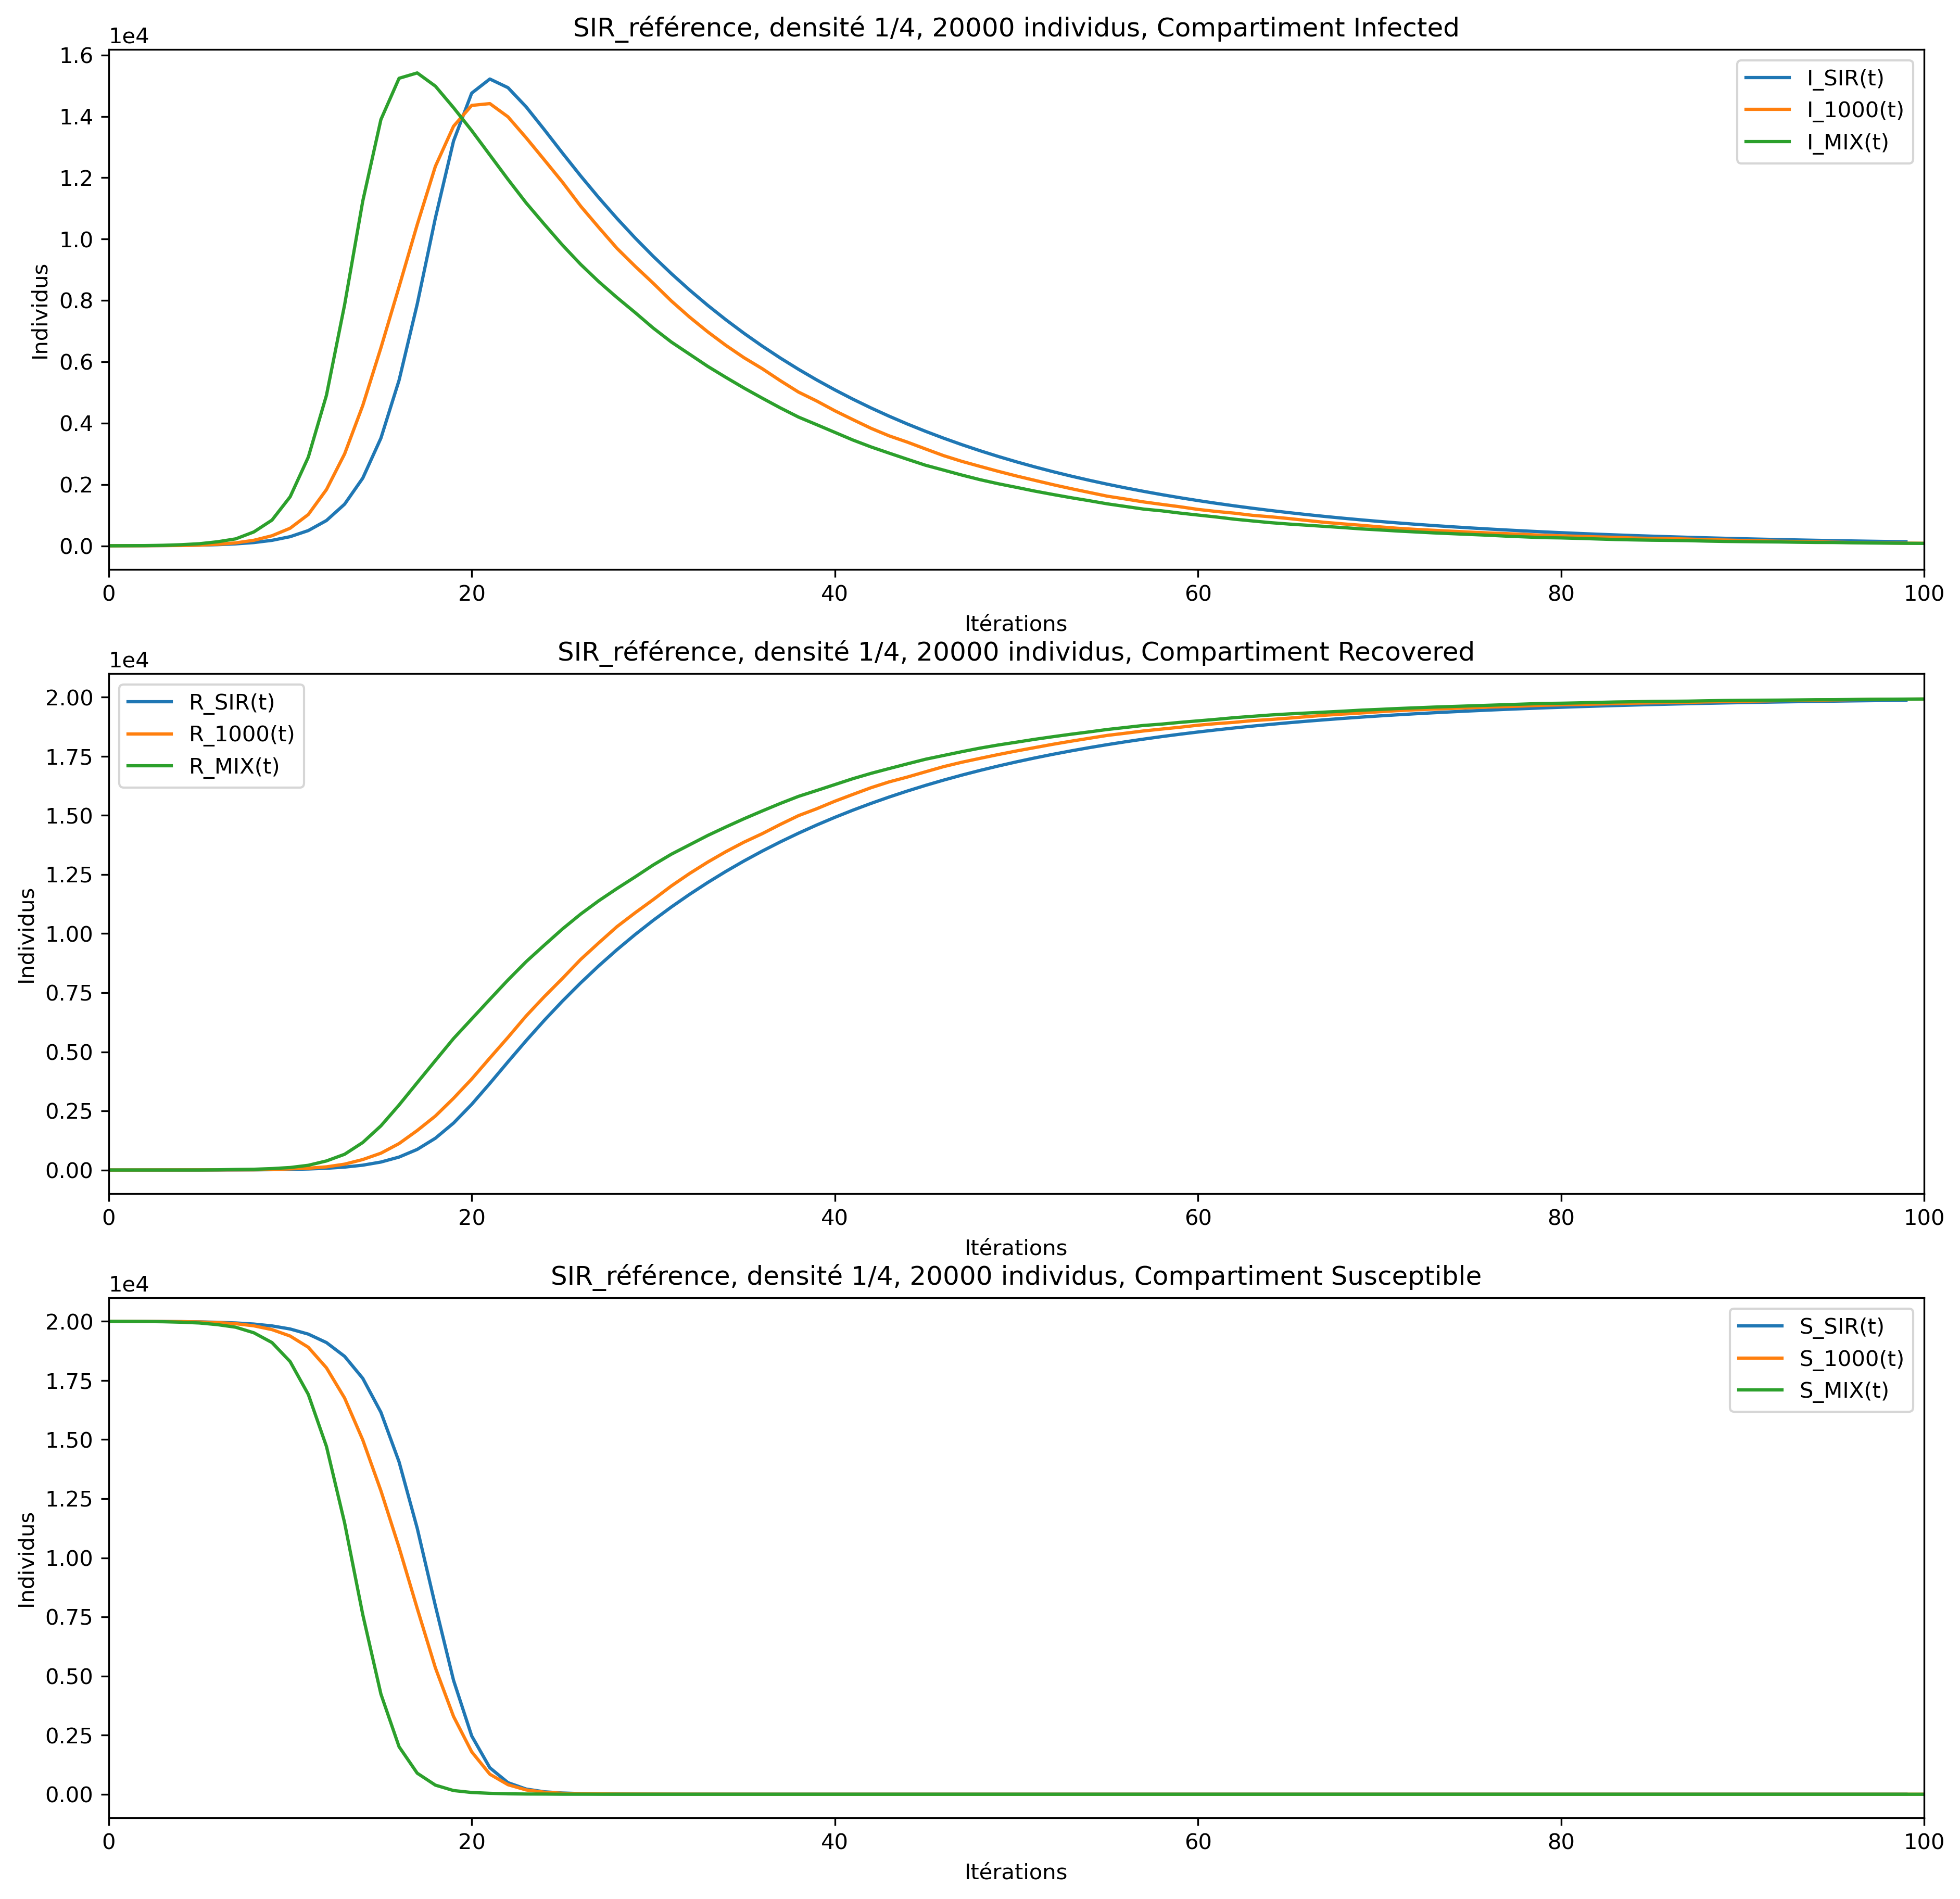
\includegraphics[width=.4\textwidth]{Images/SIR_ref_4_20.png}
	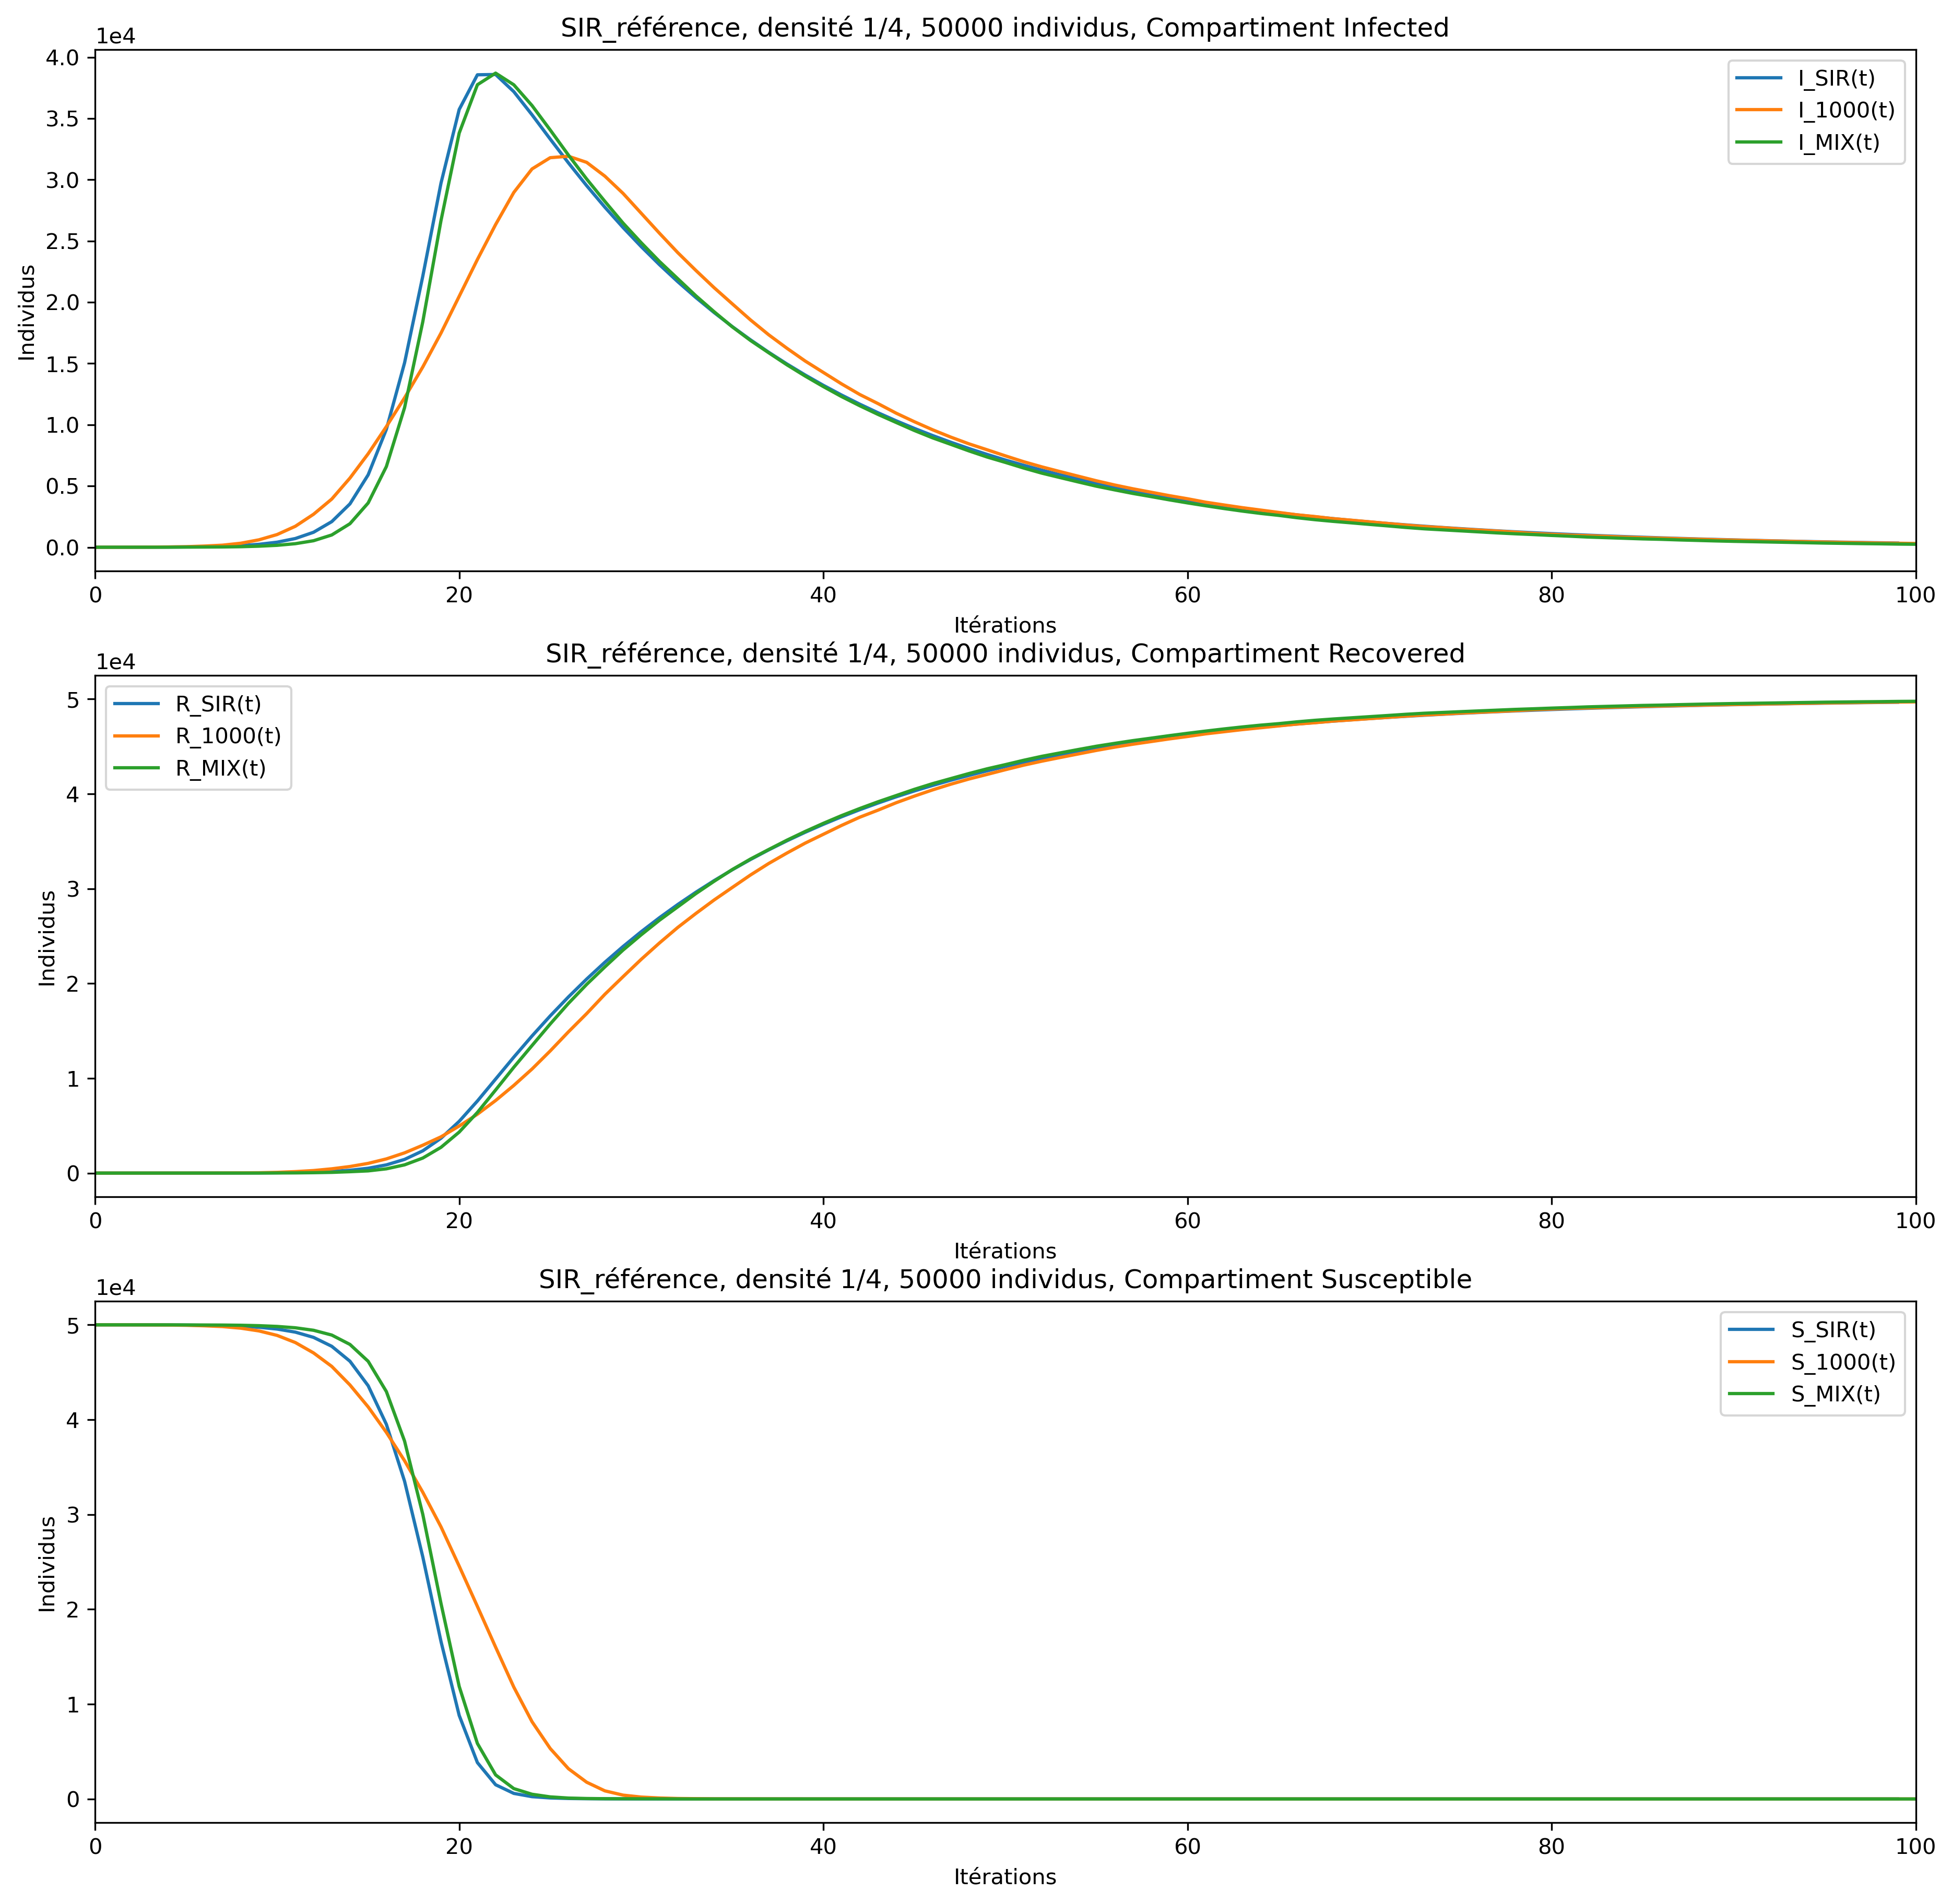
\includegraphics[width=.4\textwidth]{Images/SIR_ref_4_50.png}
	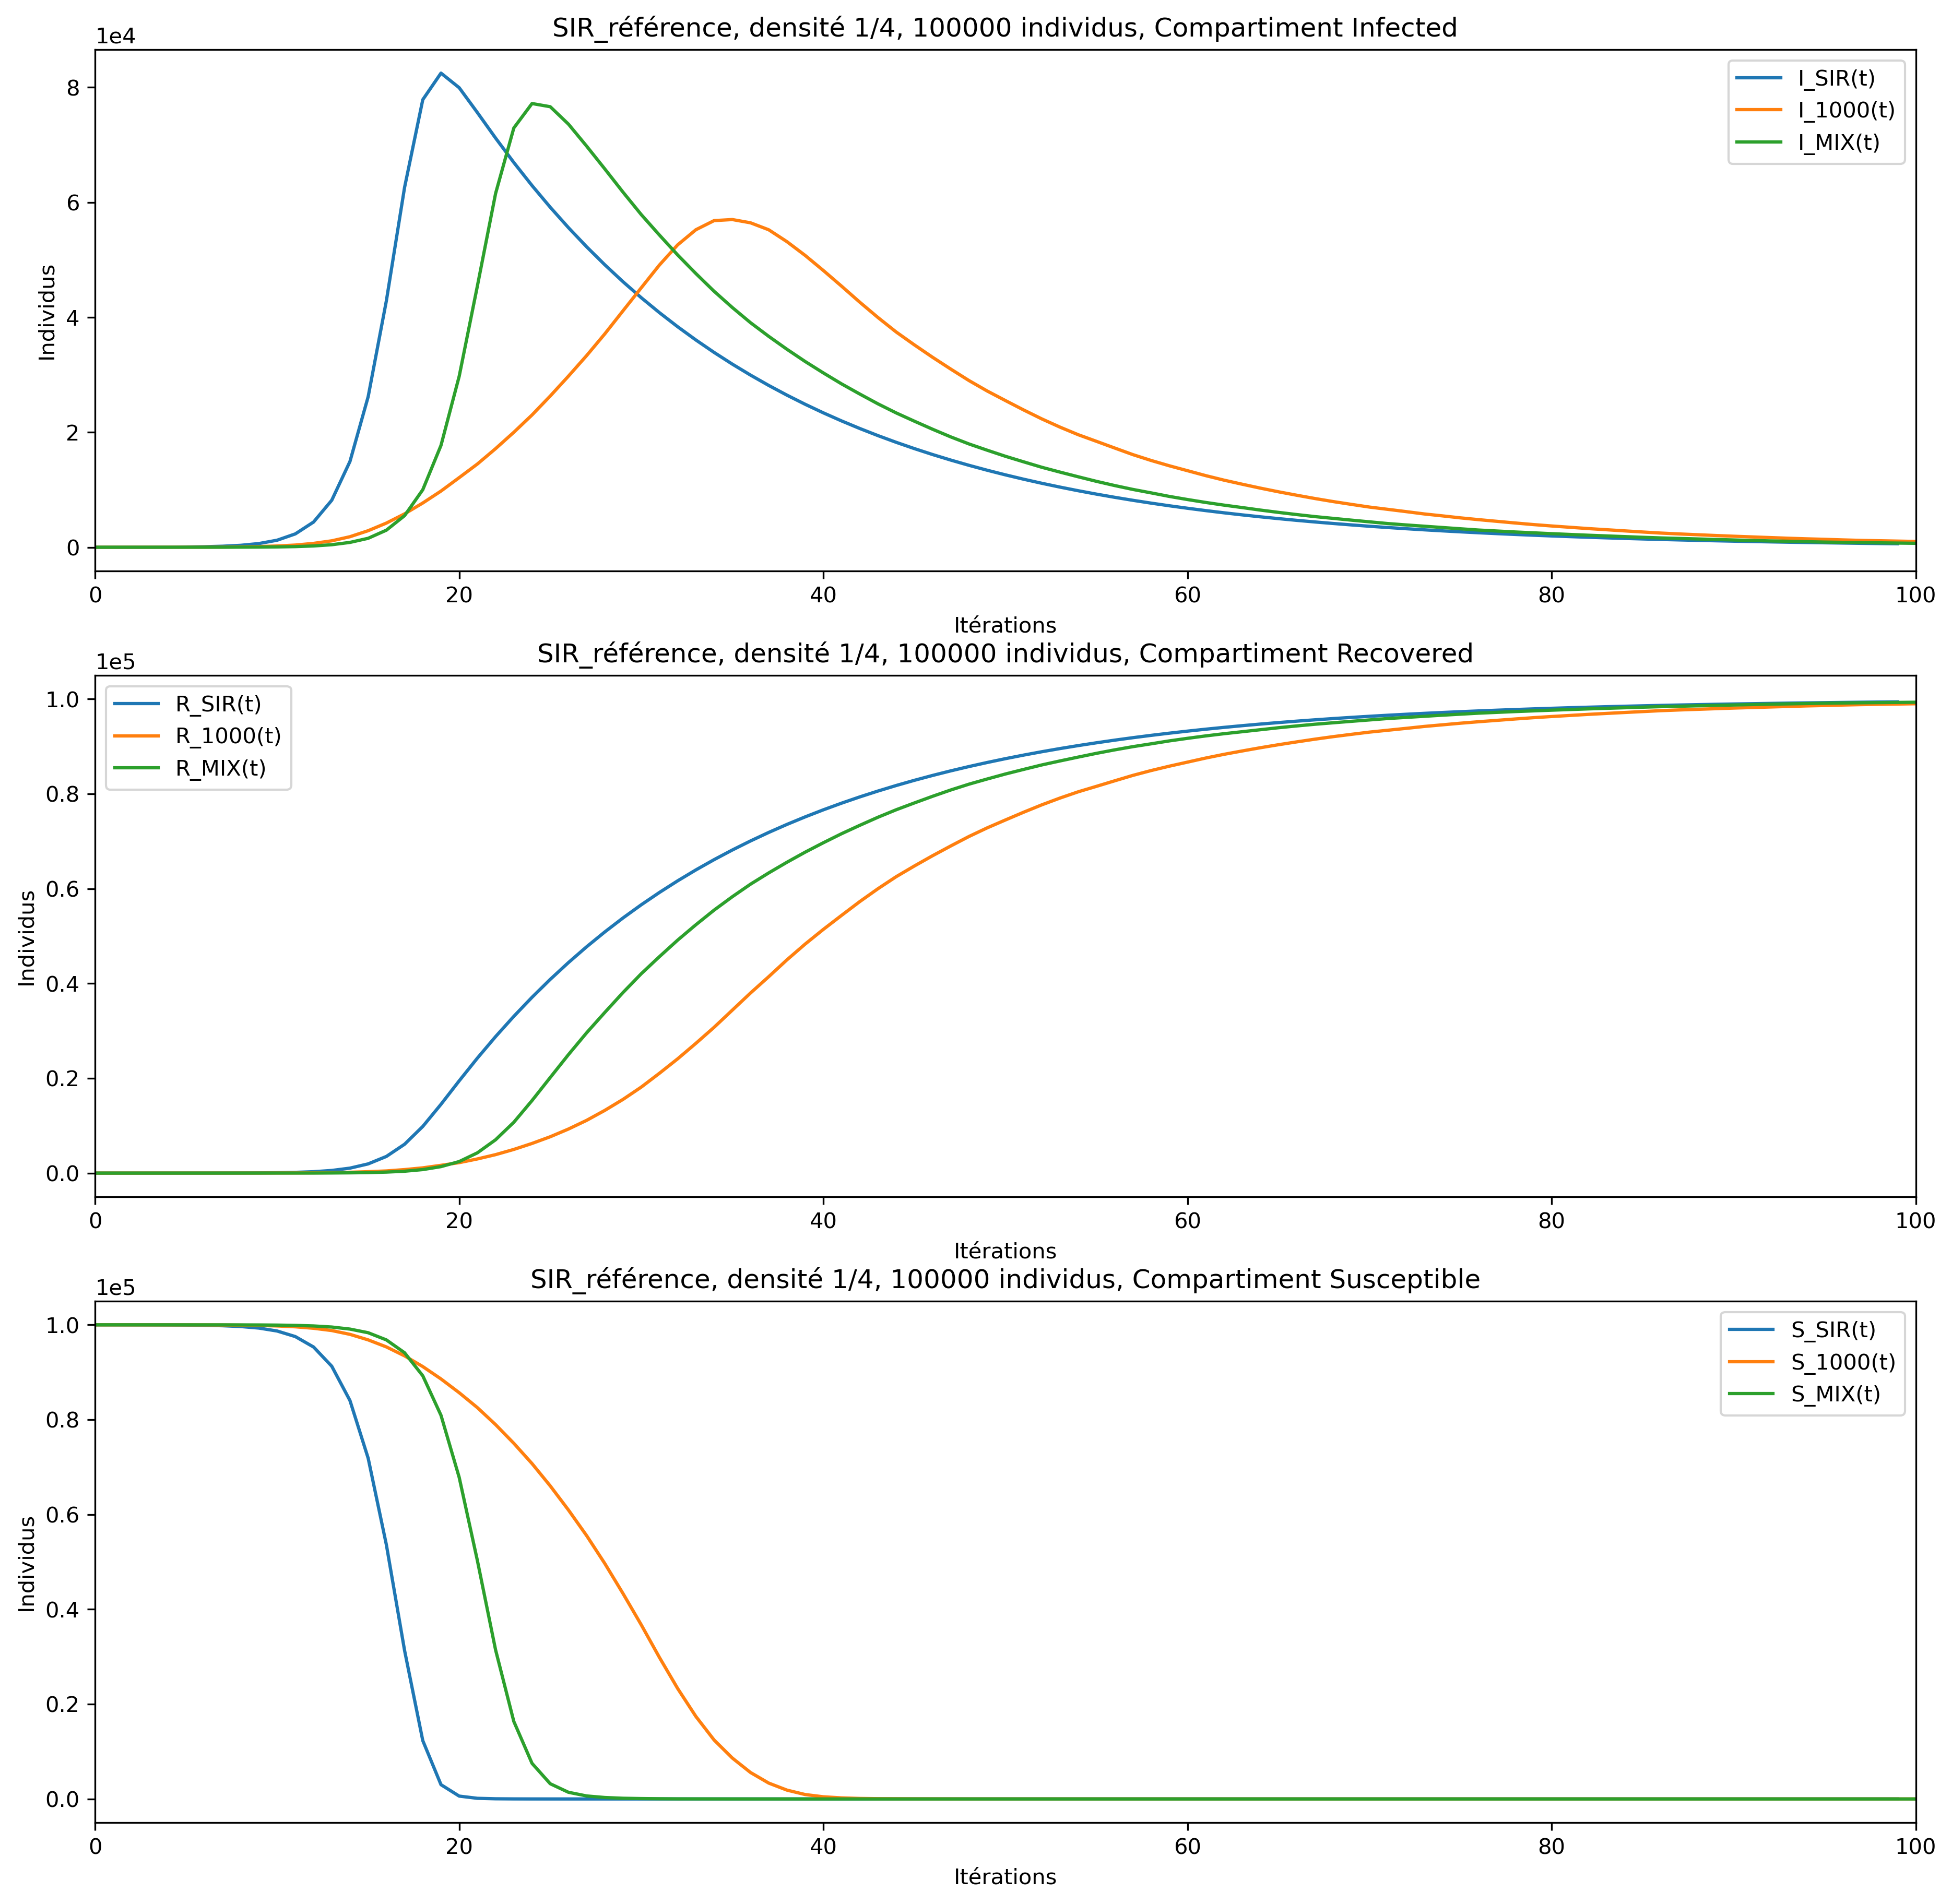
\includegraphics[width=.4\textwidth]{Images/SIR_ref_4_100.png}
	\caption{test}
\end{figure}

En densité $\frac{1}{4}$ les simulations des $1000$ mouvements tendent d'avantage vers le mélange parfait. Les courbes sont toujours plus progressives et donc les événements plus lents.

\newpage

\begin{figure}[h]
	\centering
	\captionsetup{justification=centering}
	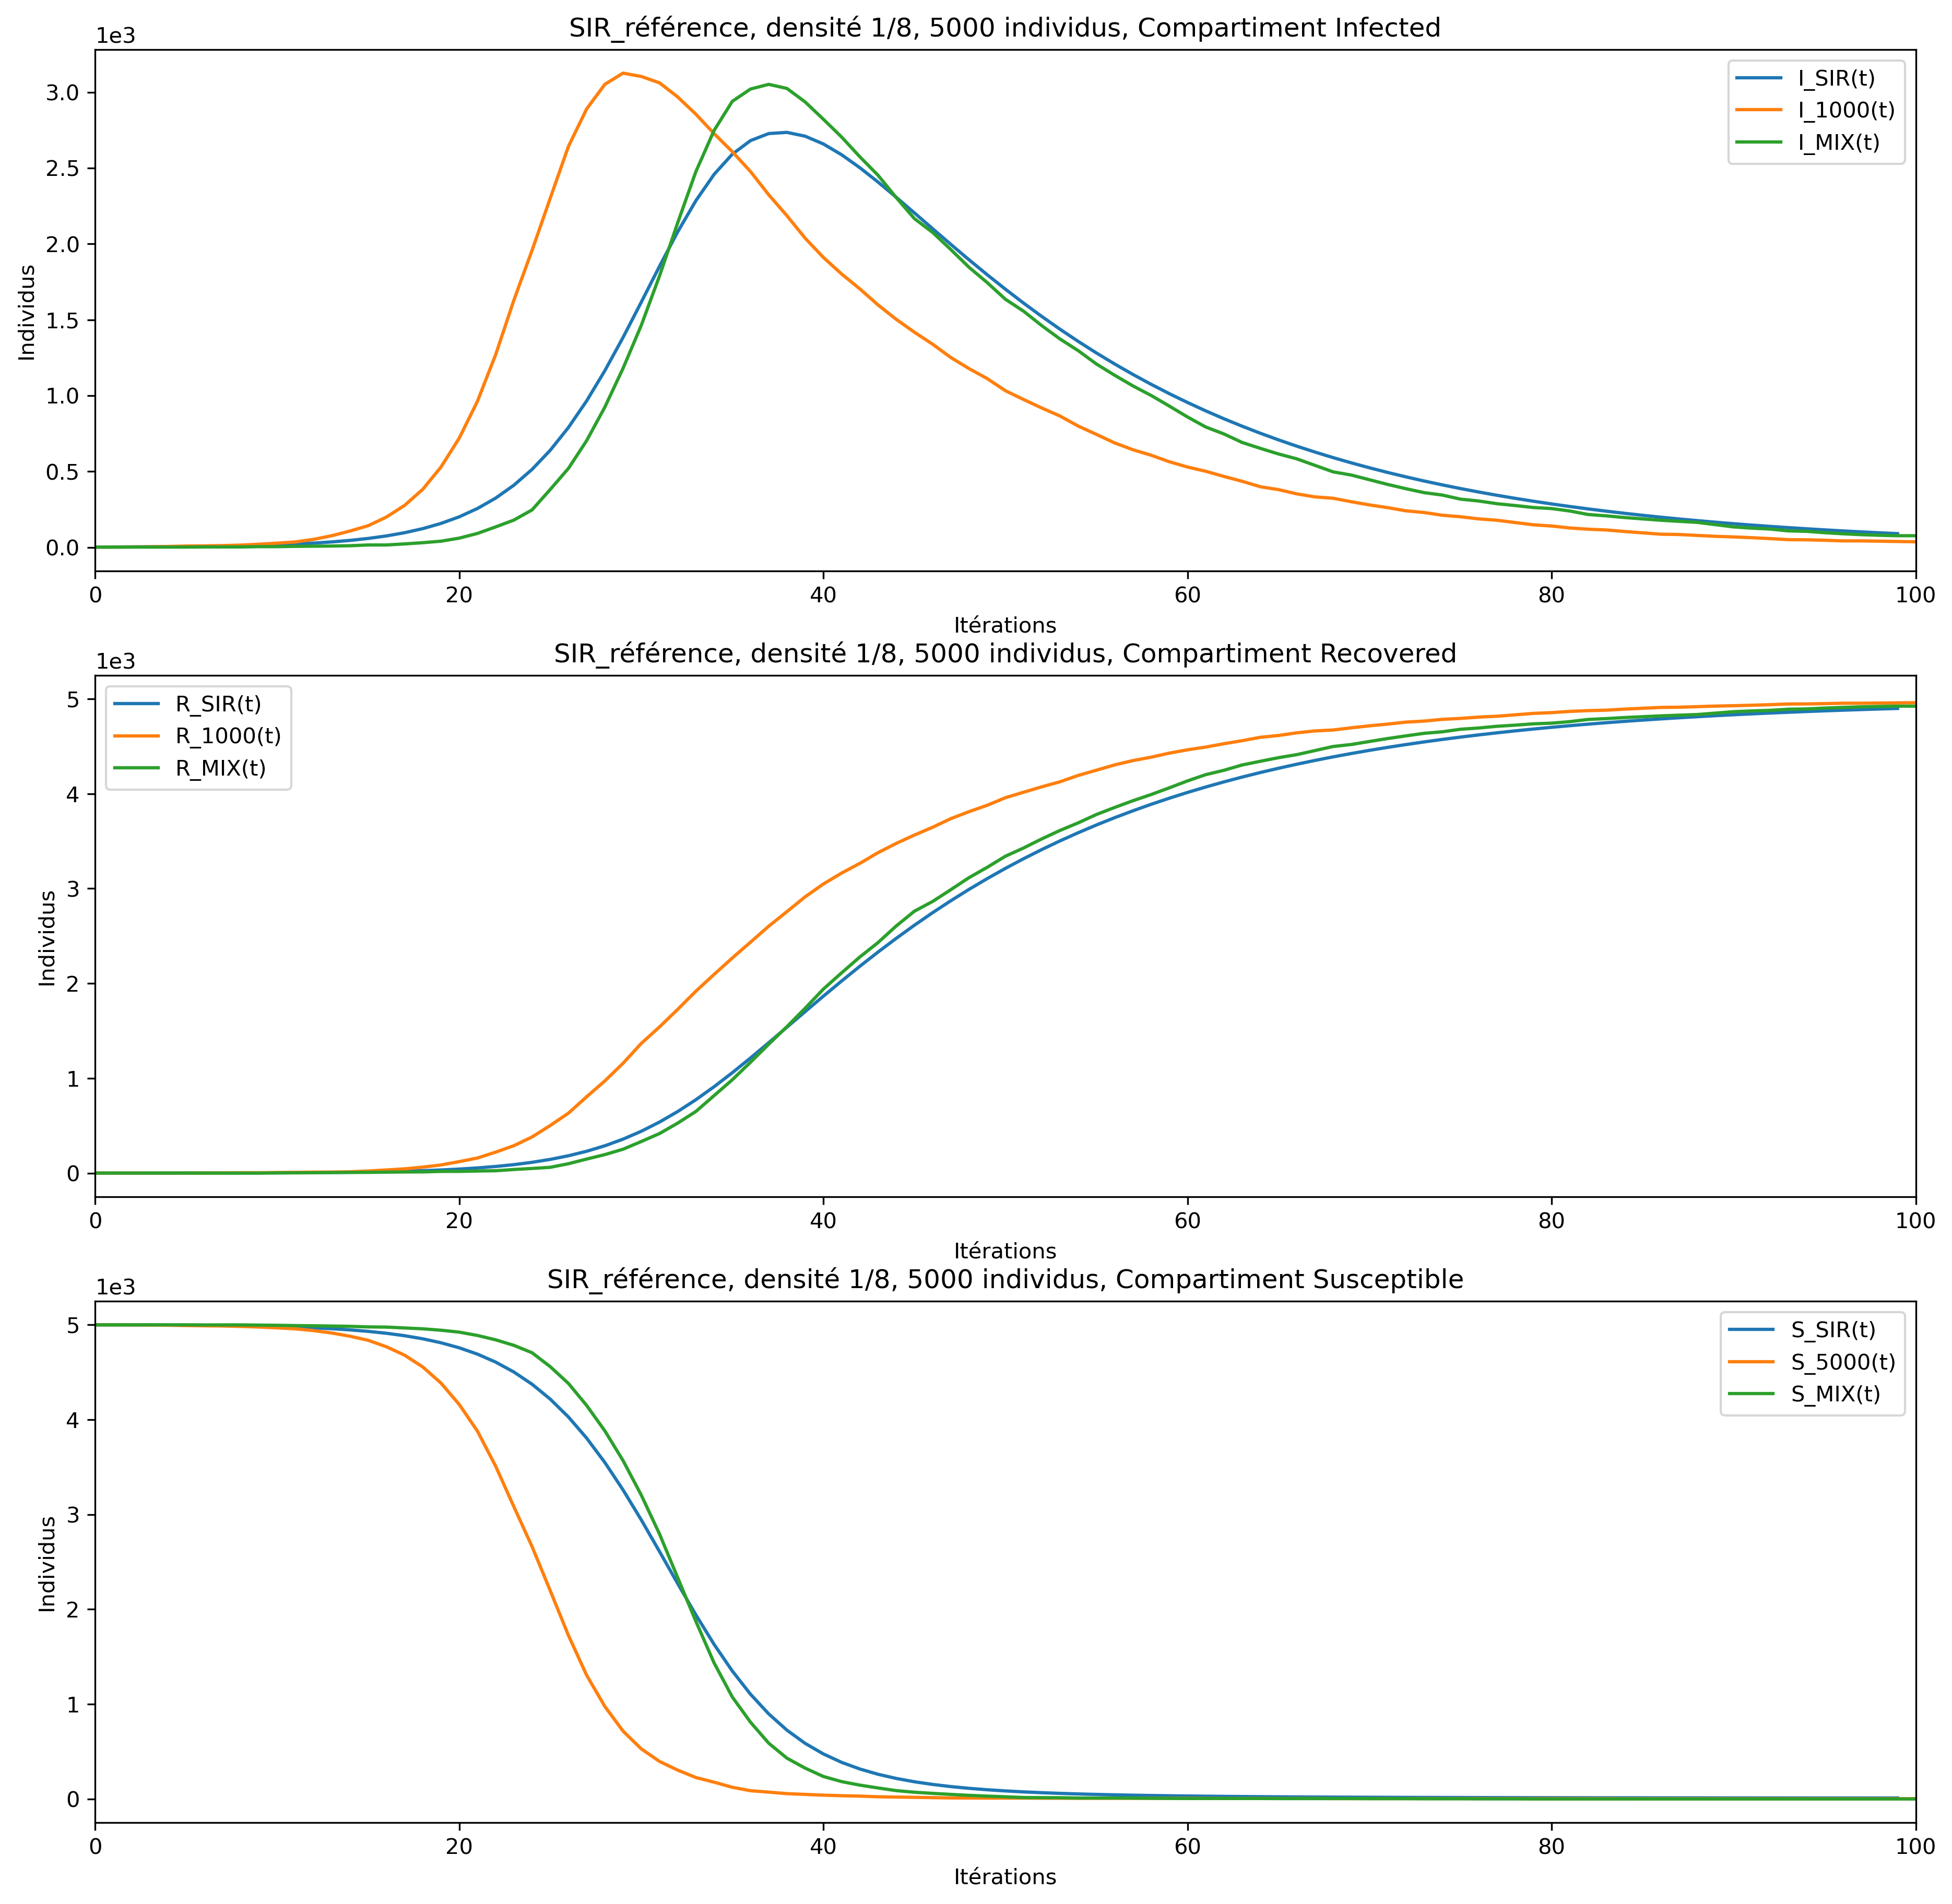
\includegraphics[width=.4\textwidth]{Images/SIR_ref_8_5.png}
	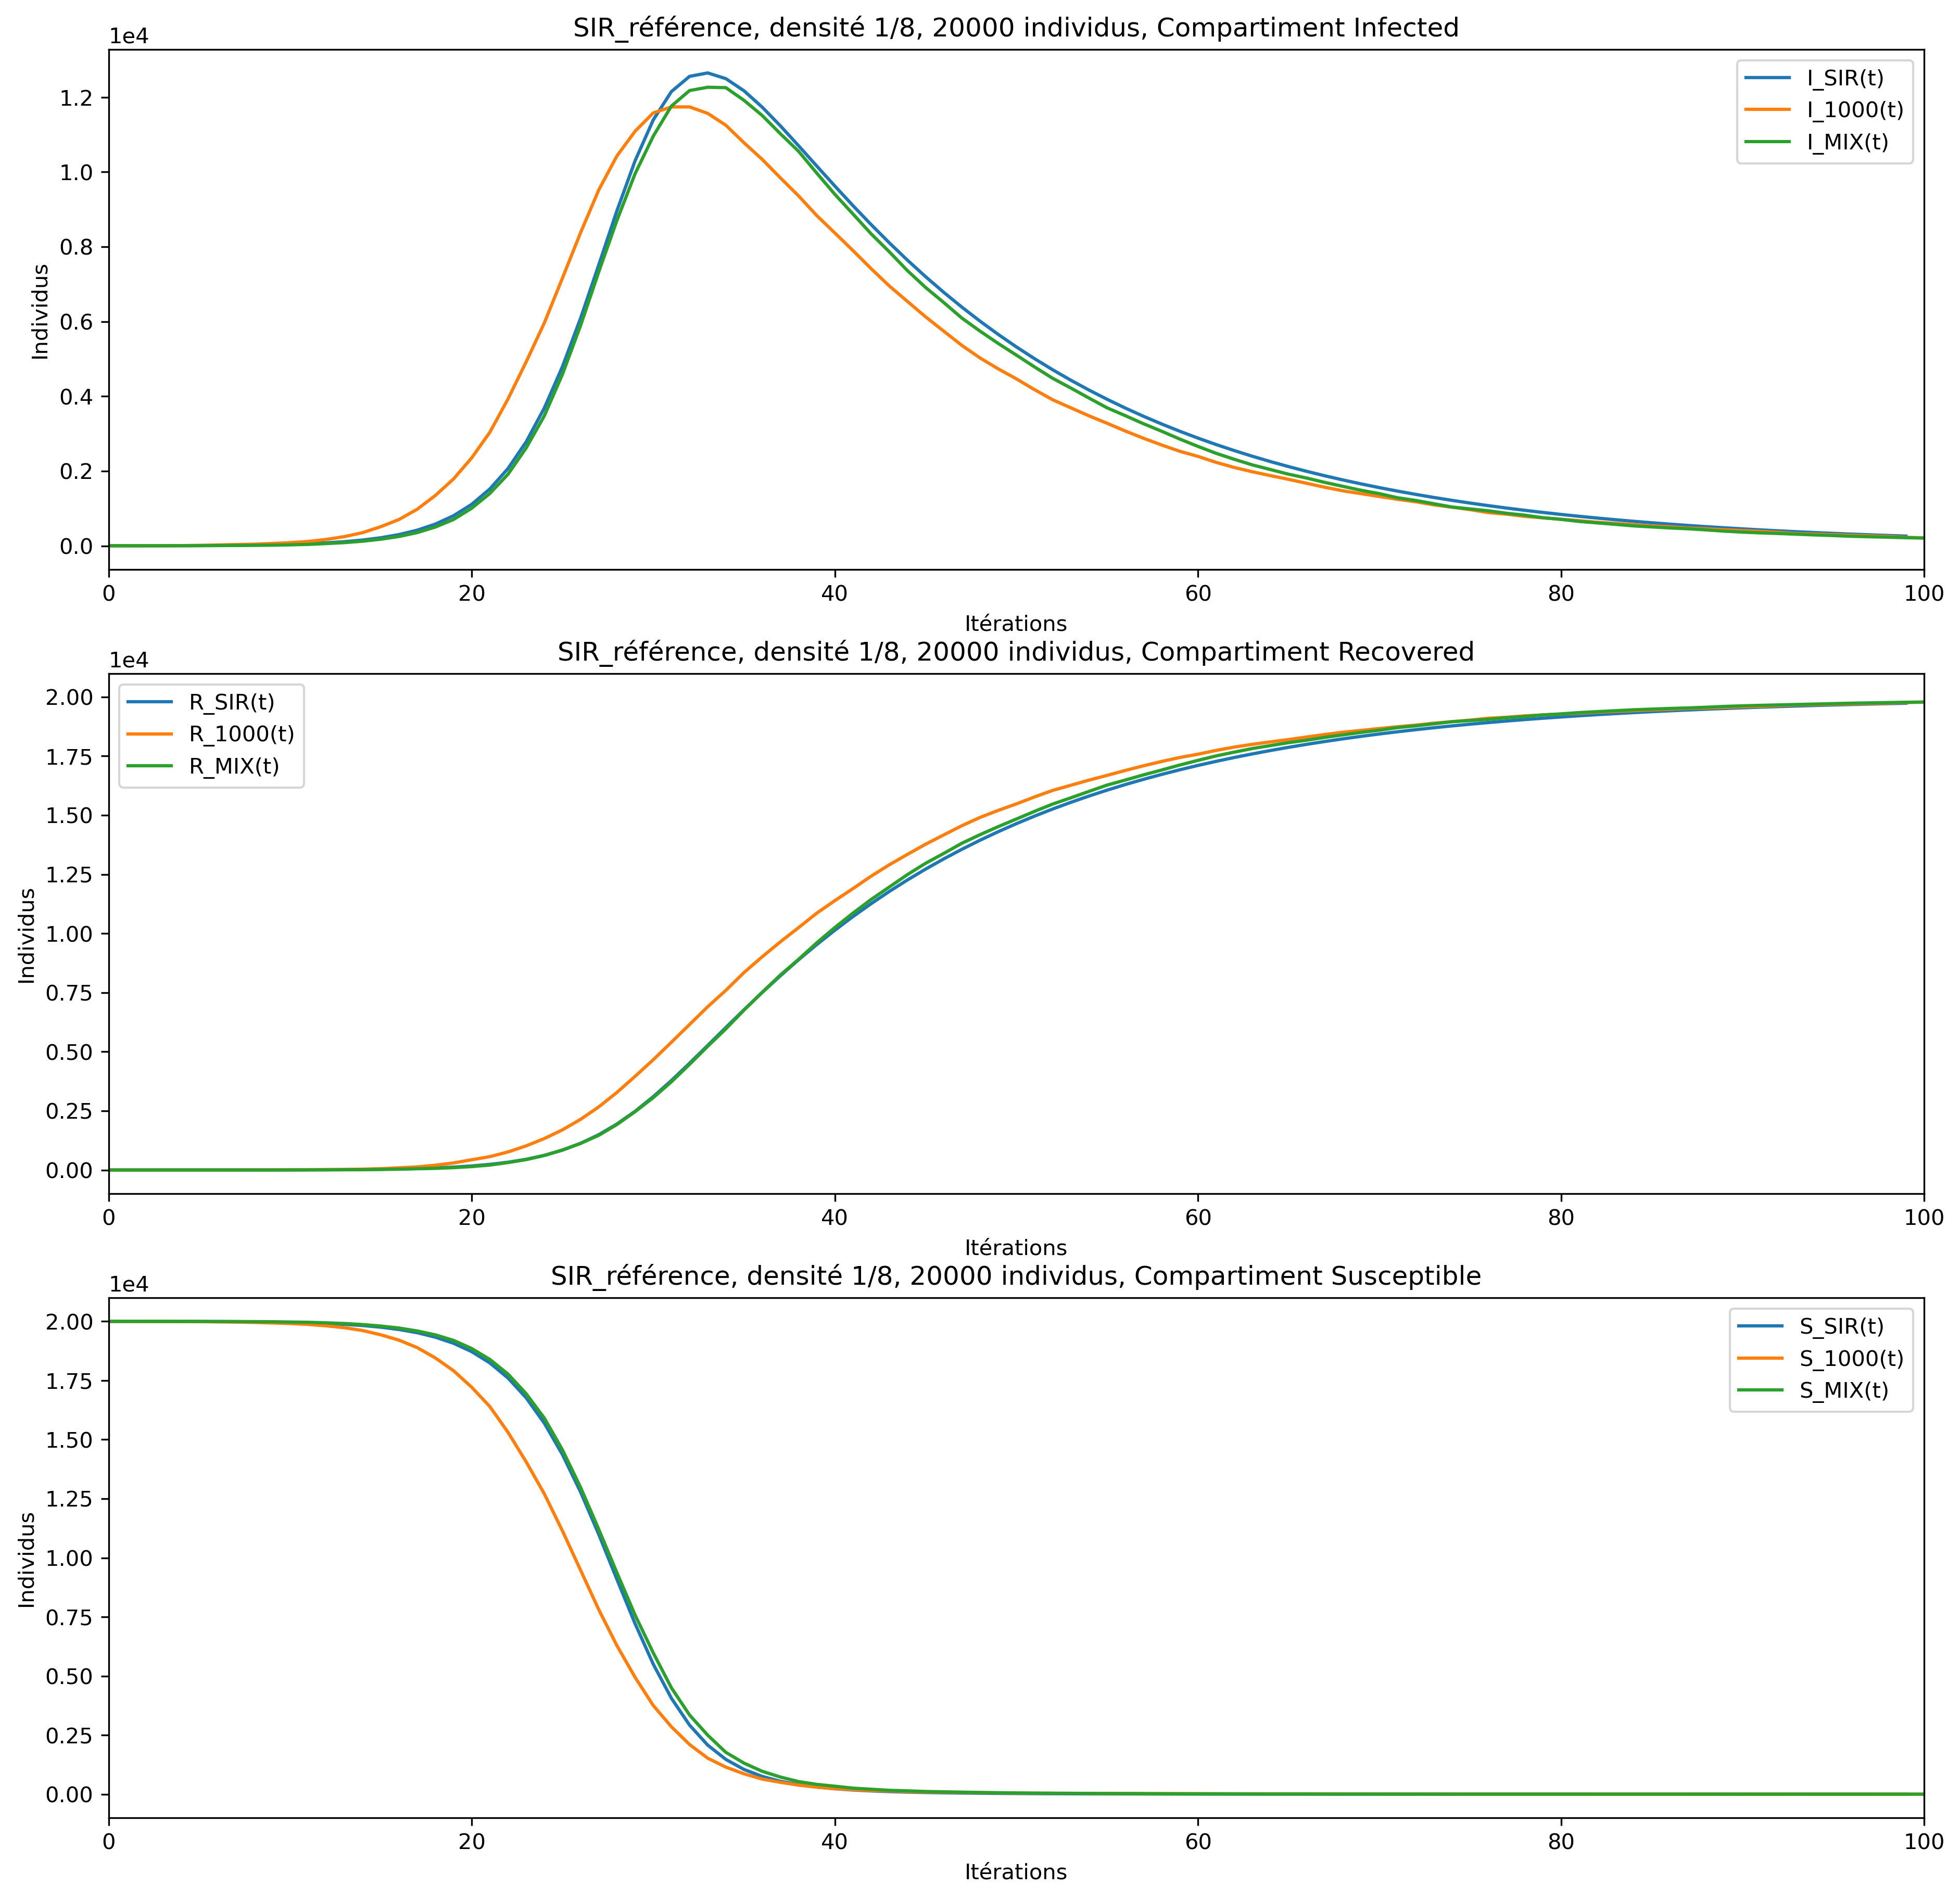
\includegraphics[width=.4\textwidth]{Images/SIR_ref_8_20.png}
	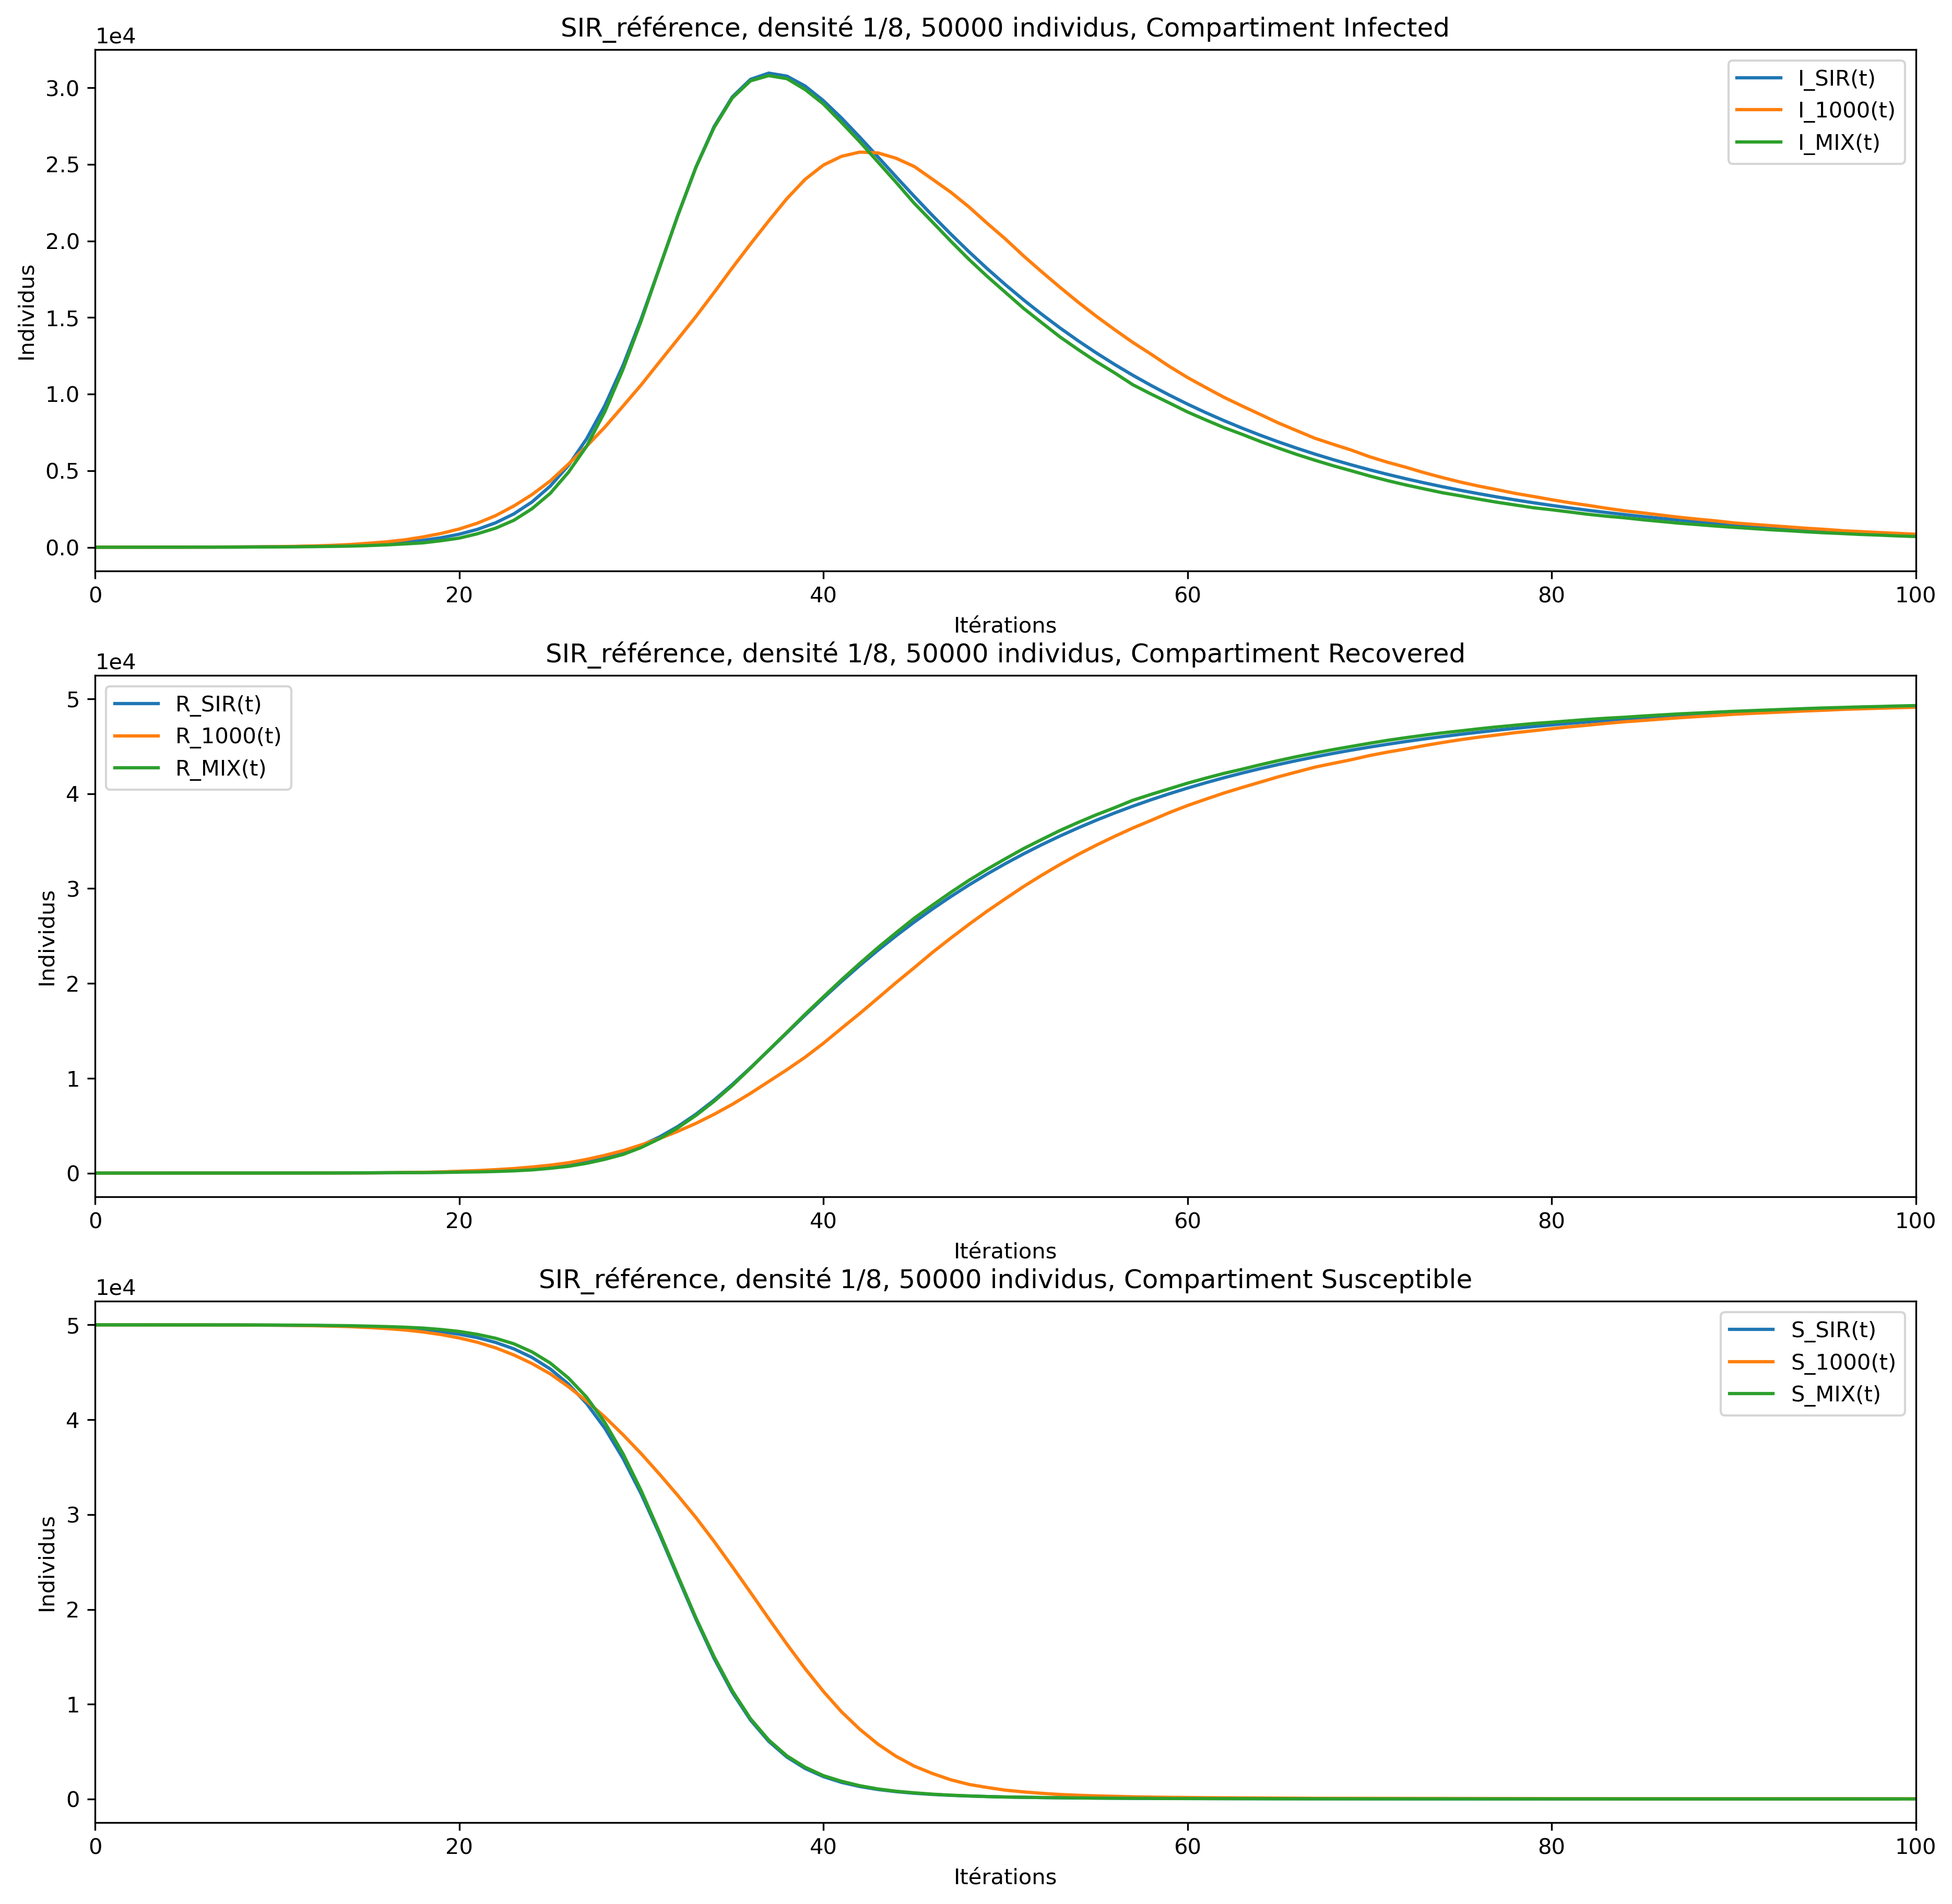
\includegraphics[width=.4\textwidth]{Images/SIR_ref_8_50.png}
	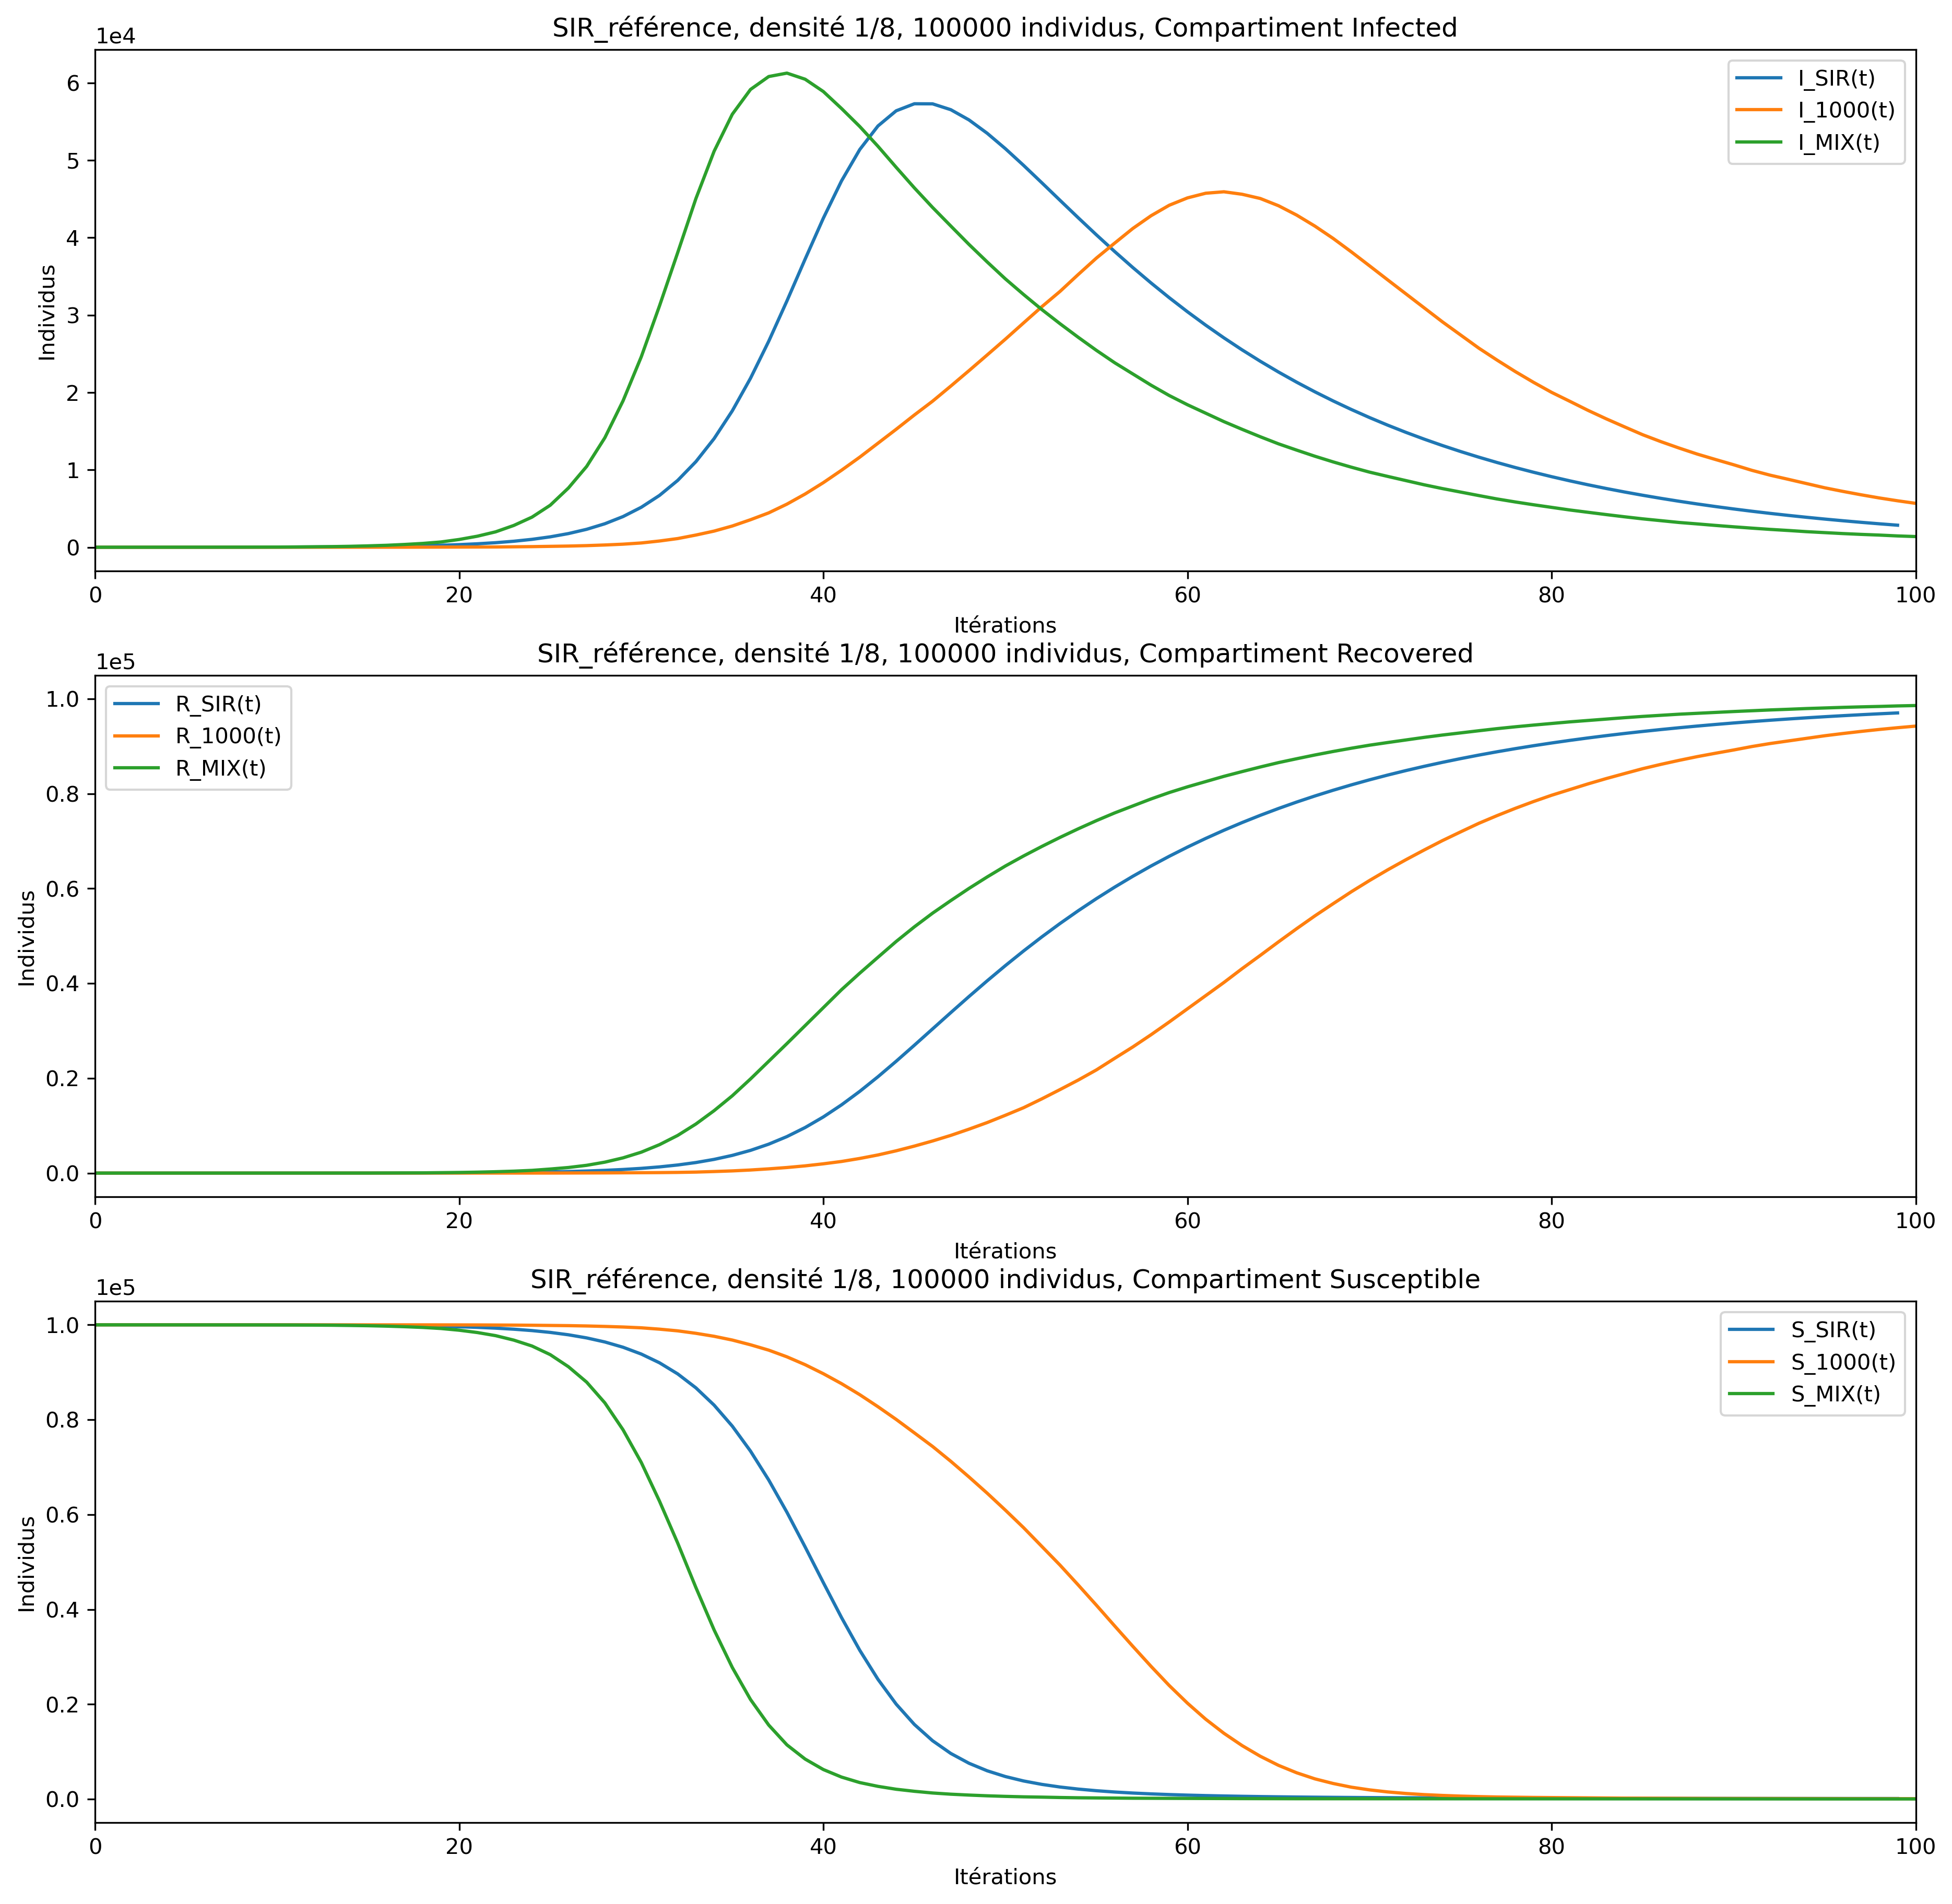
\includegraphics[width=.4\textwidth]{Images/SIR_ref_8_100.png}
	\caption{test}
\end{figure}

En plus de retrouver les mêmes comportements qu'observés précédemment, il y a un nouveau phénomène que nous pouvons observer ici. Ce phénomène est particulièrement présent dans les simulations à $5000$, $20000$ et $100000$ individus. Nous remarquons que la croissance des courbes pour les simulations de mélange parfait sont plus rapides que le modèle mathématique SIR. Ce comportement est dû au fait que nos simulations peuvent nécessiter d'un temps de latence avant l'émergence d'un événement. Alors que au contraire le modèle SIR n'est pas victime de cette latence.\\

Par conséquent, pour joindre le modèle SIR aux simulations il faut prendre en compte le temps de latence et l'ajouter au modèle SI artificiellement. Ce temps de latence est particulièrement présent sur les systèmes peu denses car dans ces configurations les pandémies peuvent prendre du temps à apparaitre. Ce phénomène est étudié dans un autre chapitre.

\newpage

\begin{figure}[h]
	\centering
	\captionsetup{justification=centering}
	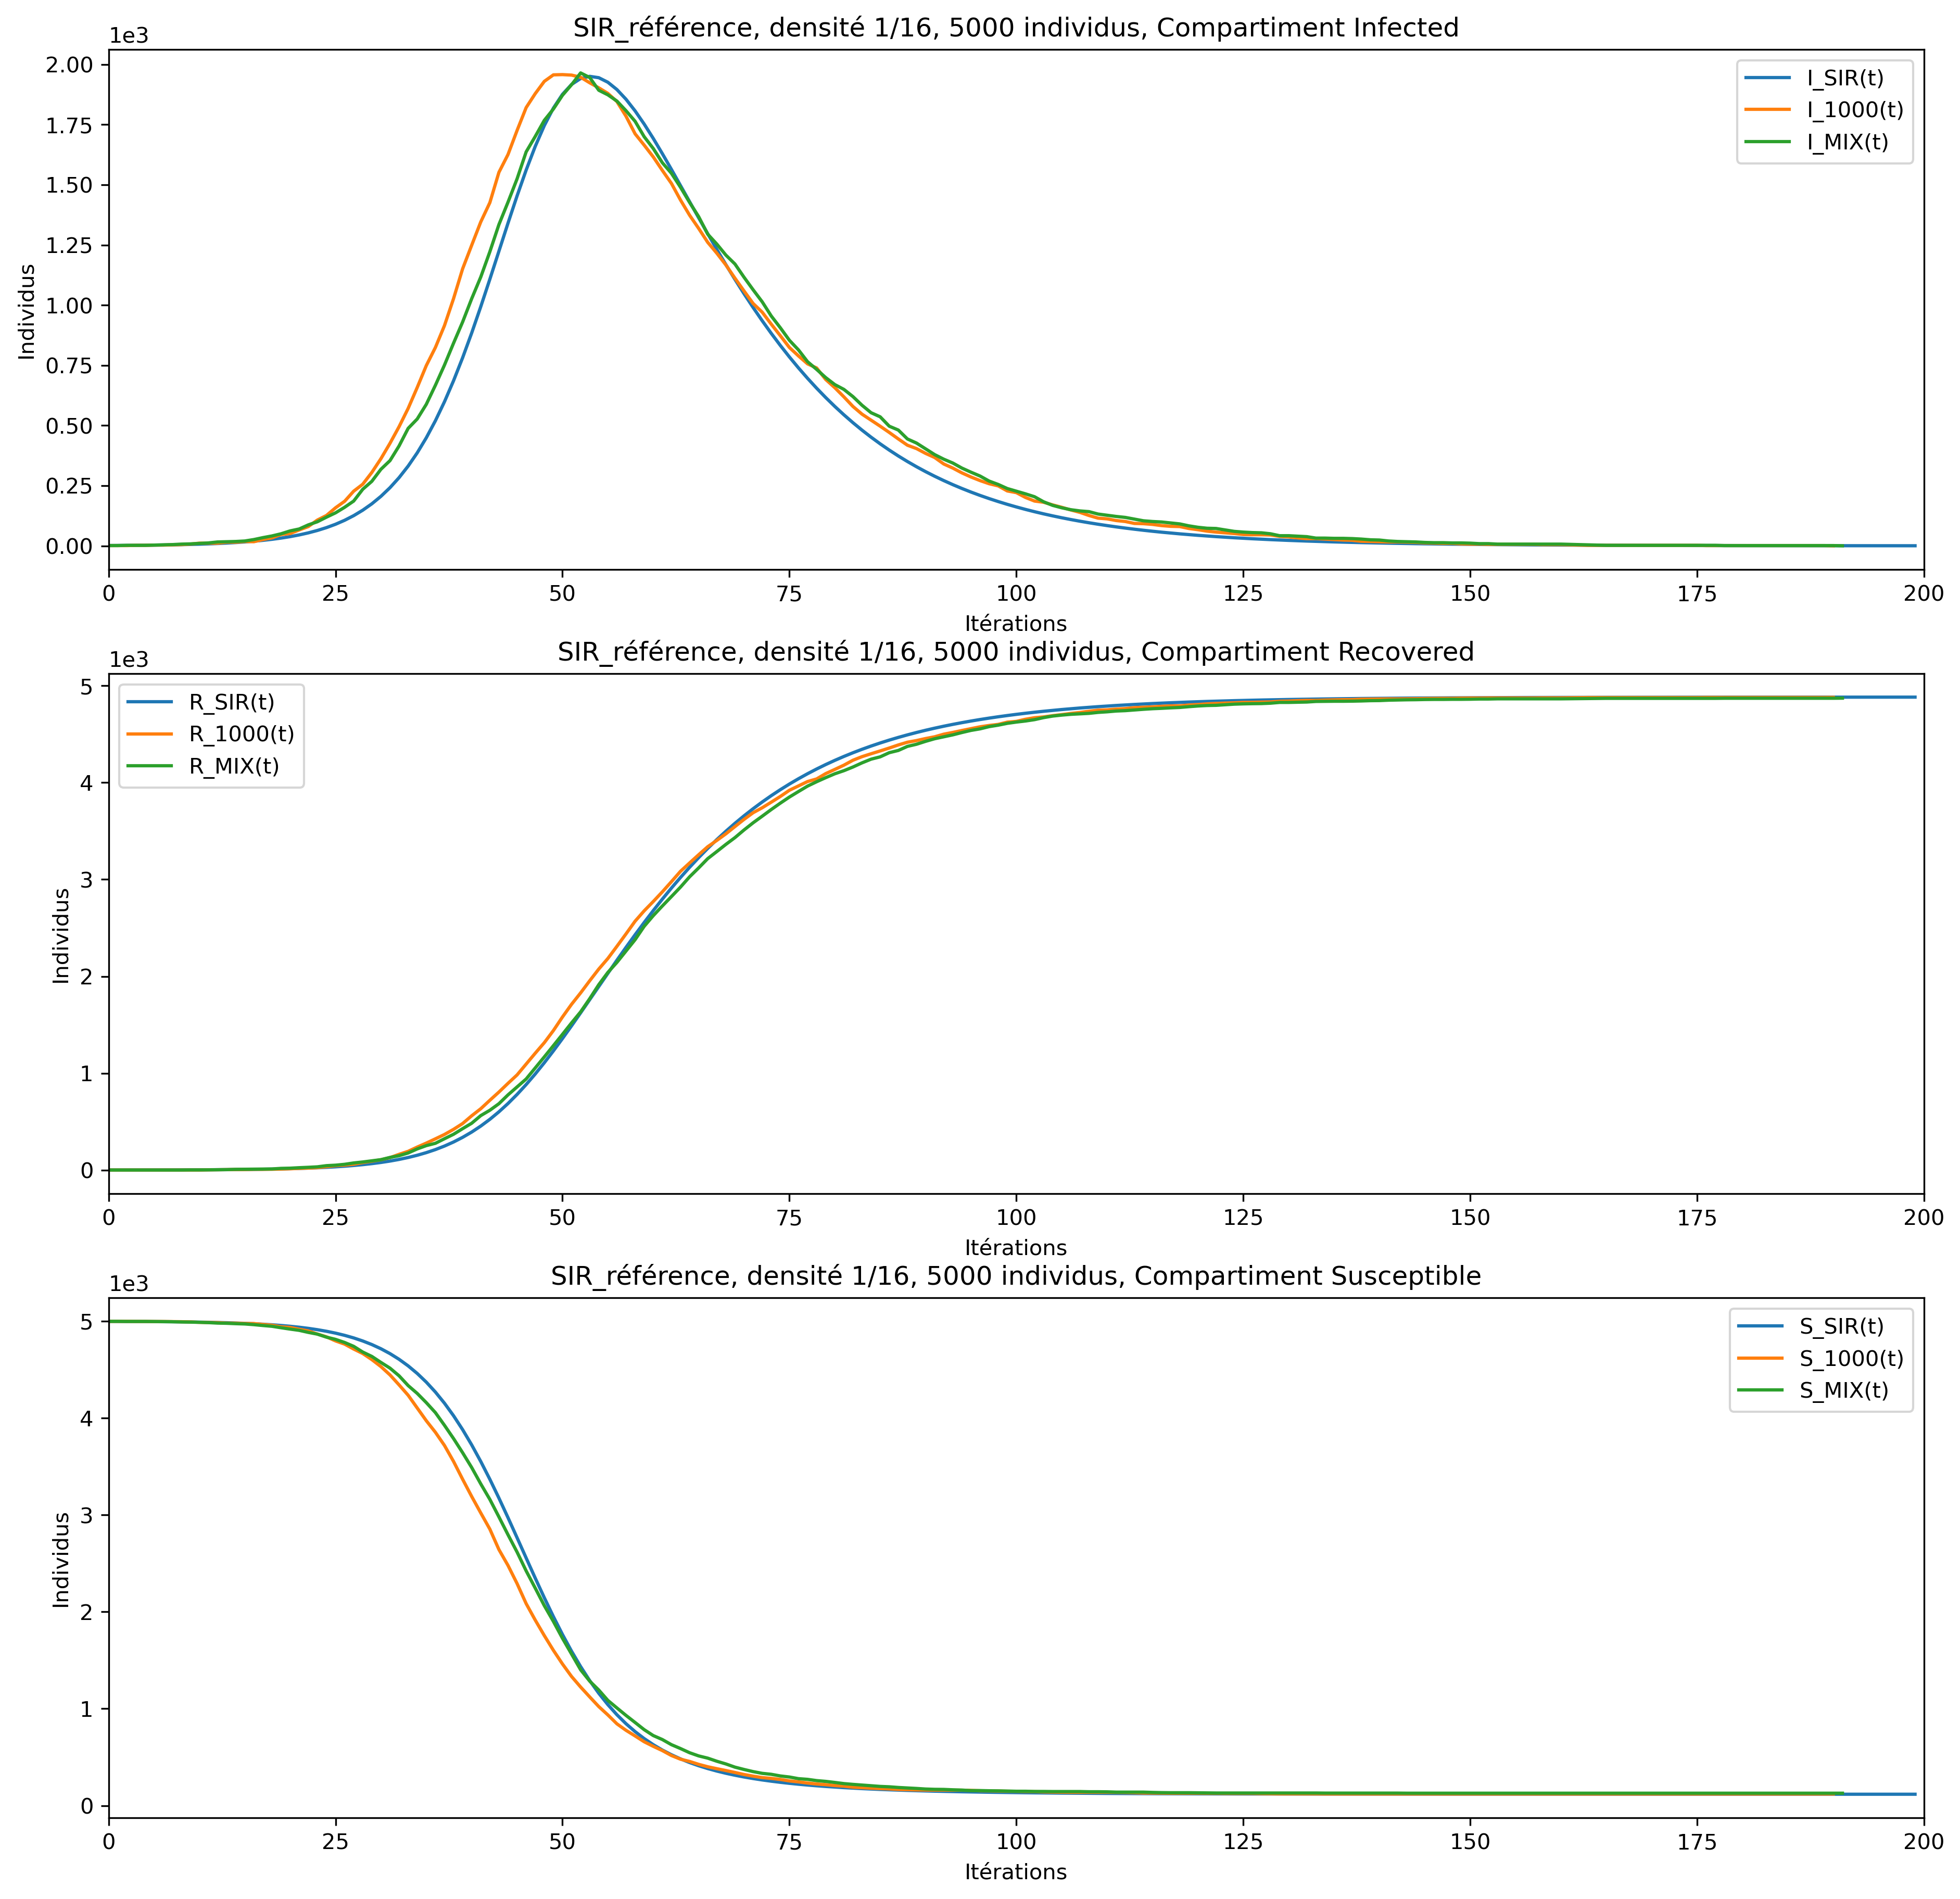
\includegraphics[width=.4\textwidth]{Images/SIR_ref_16_5.png}
	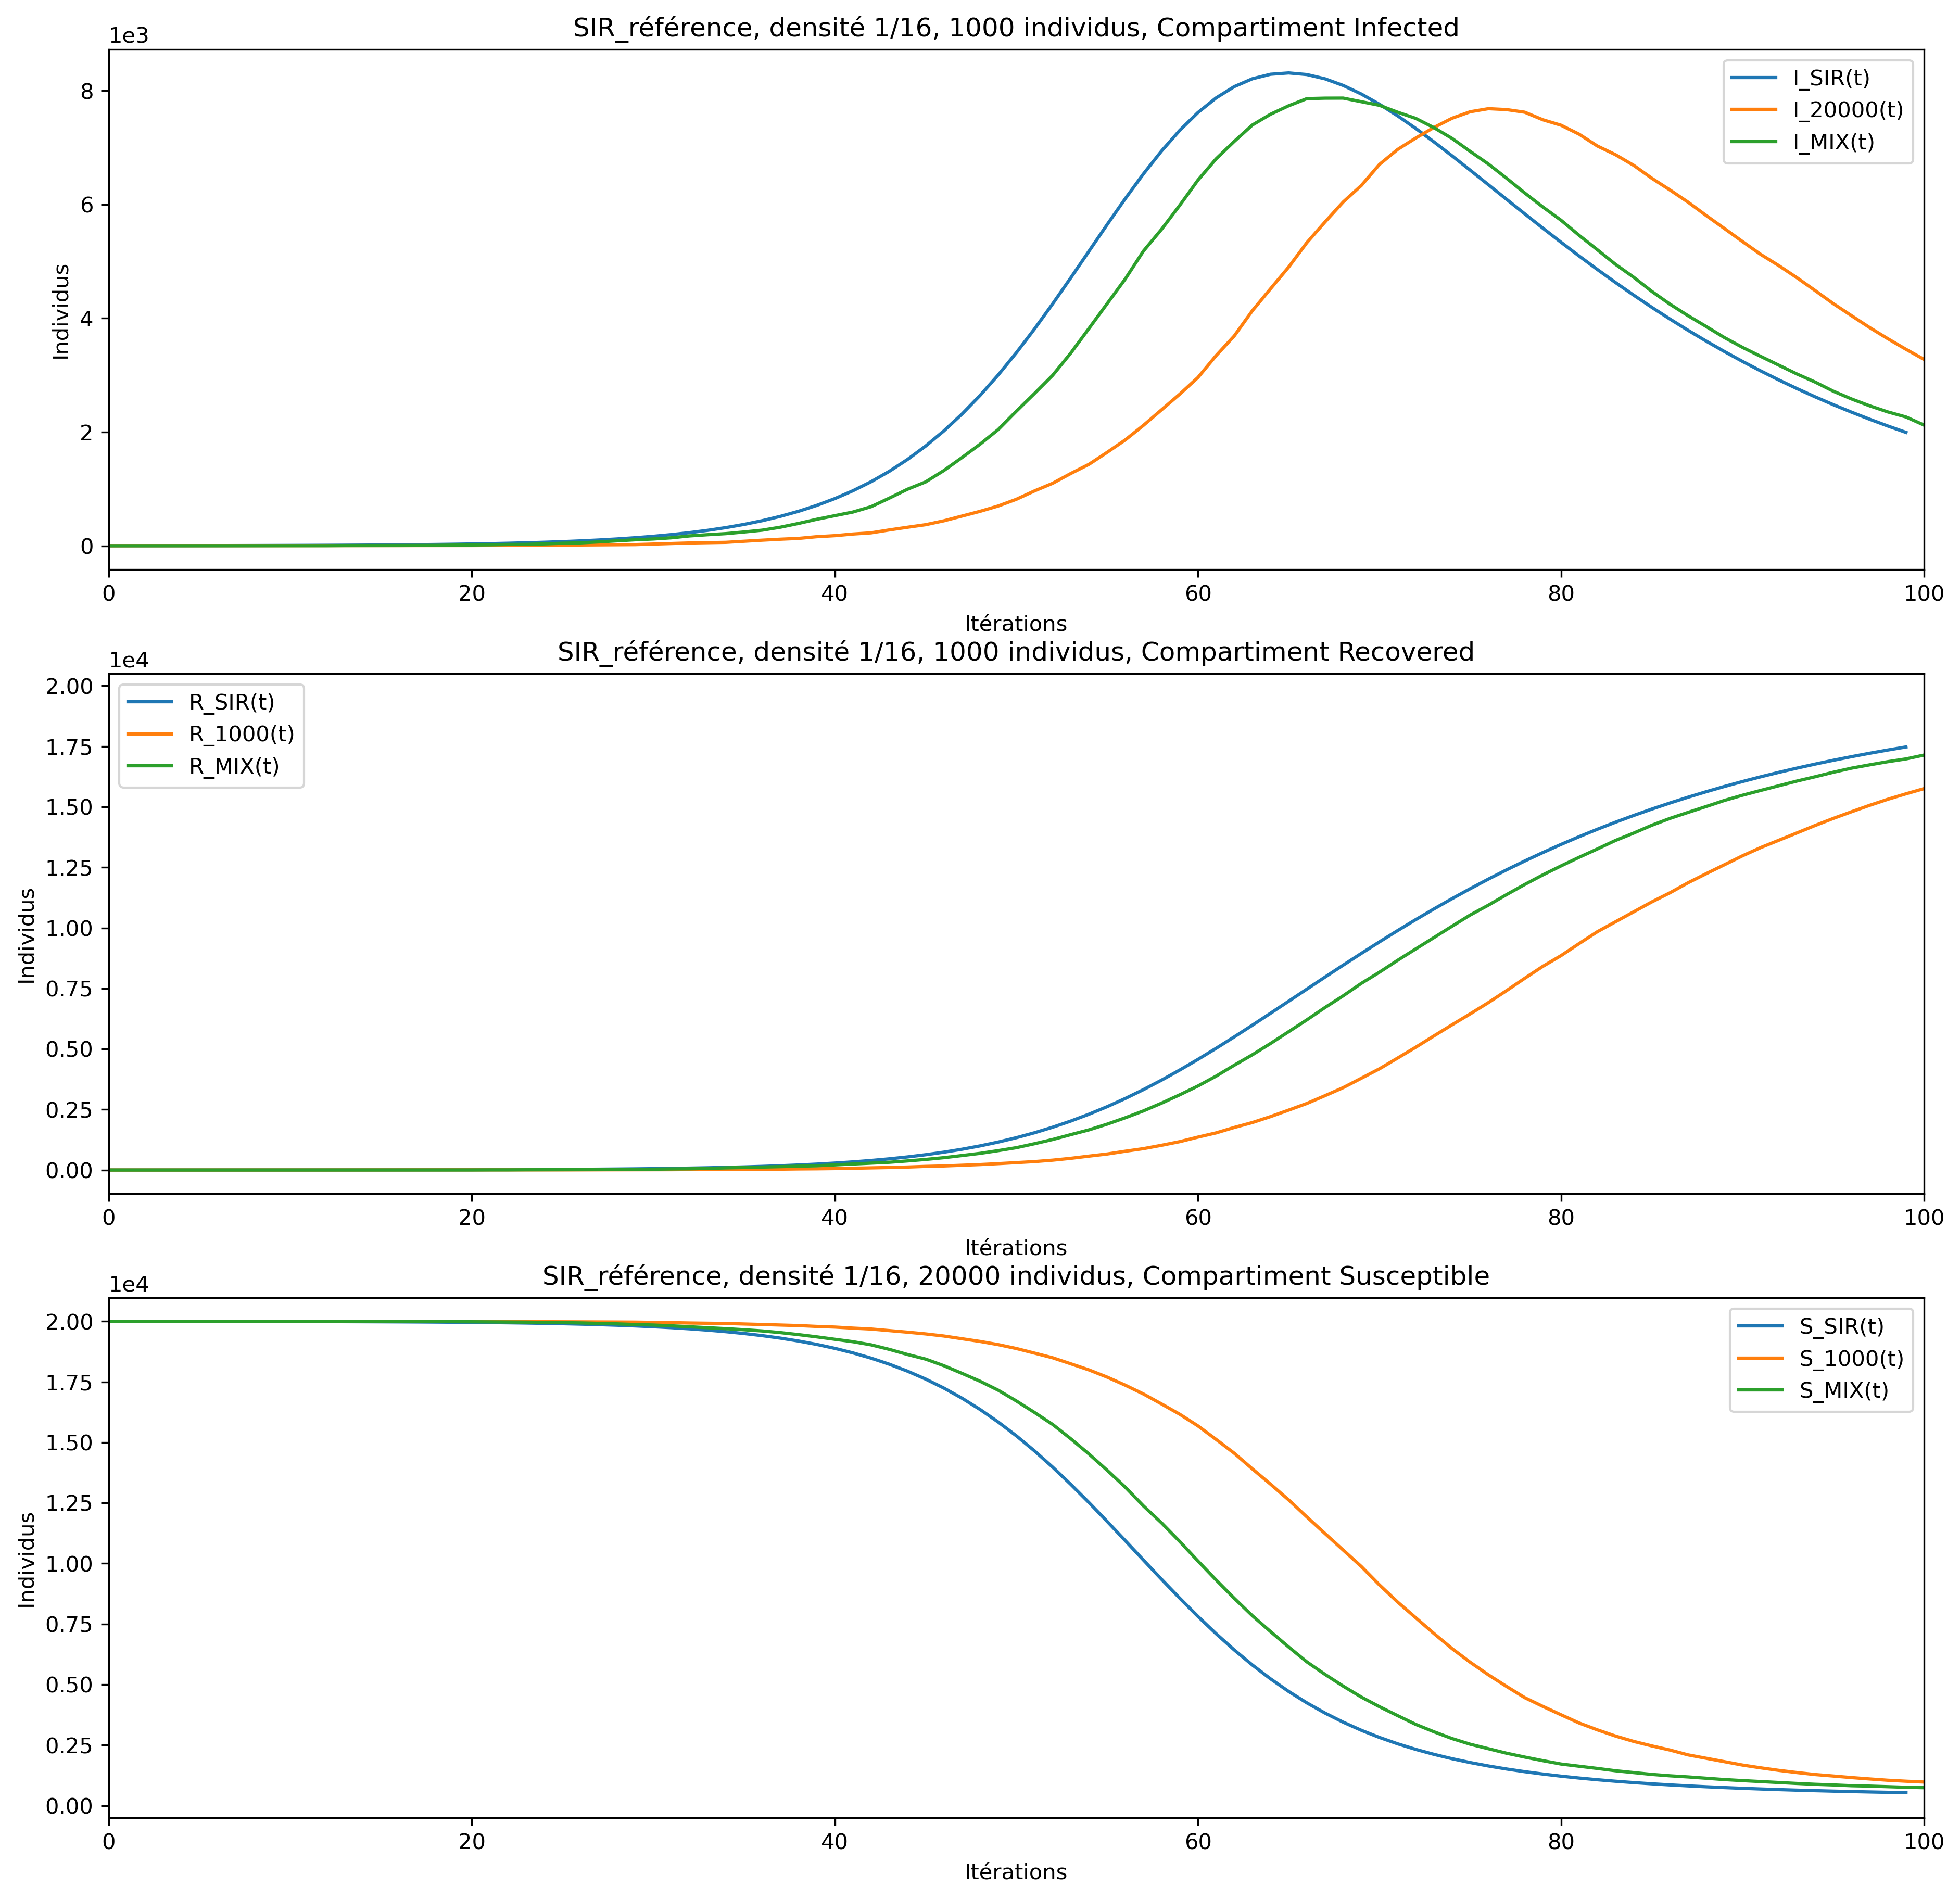
\includegraphics[width=.4\textwidth]{Images/SIR_ref_16_20.png}
	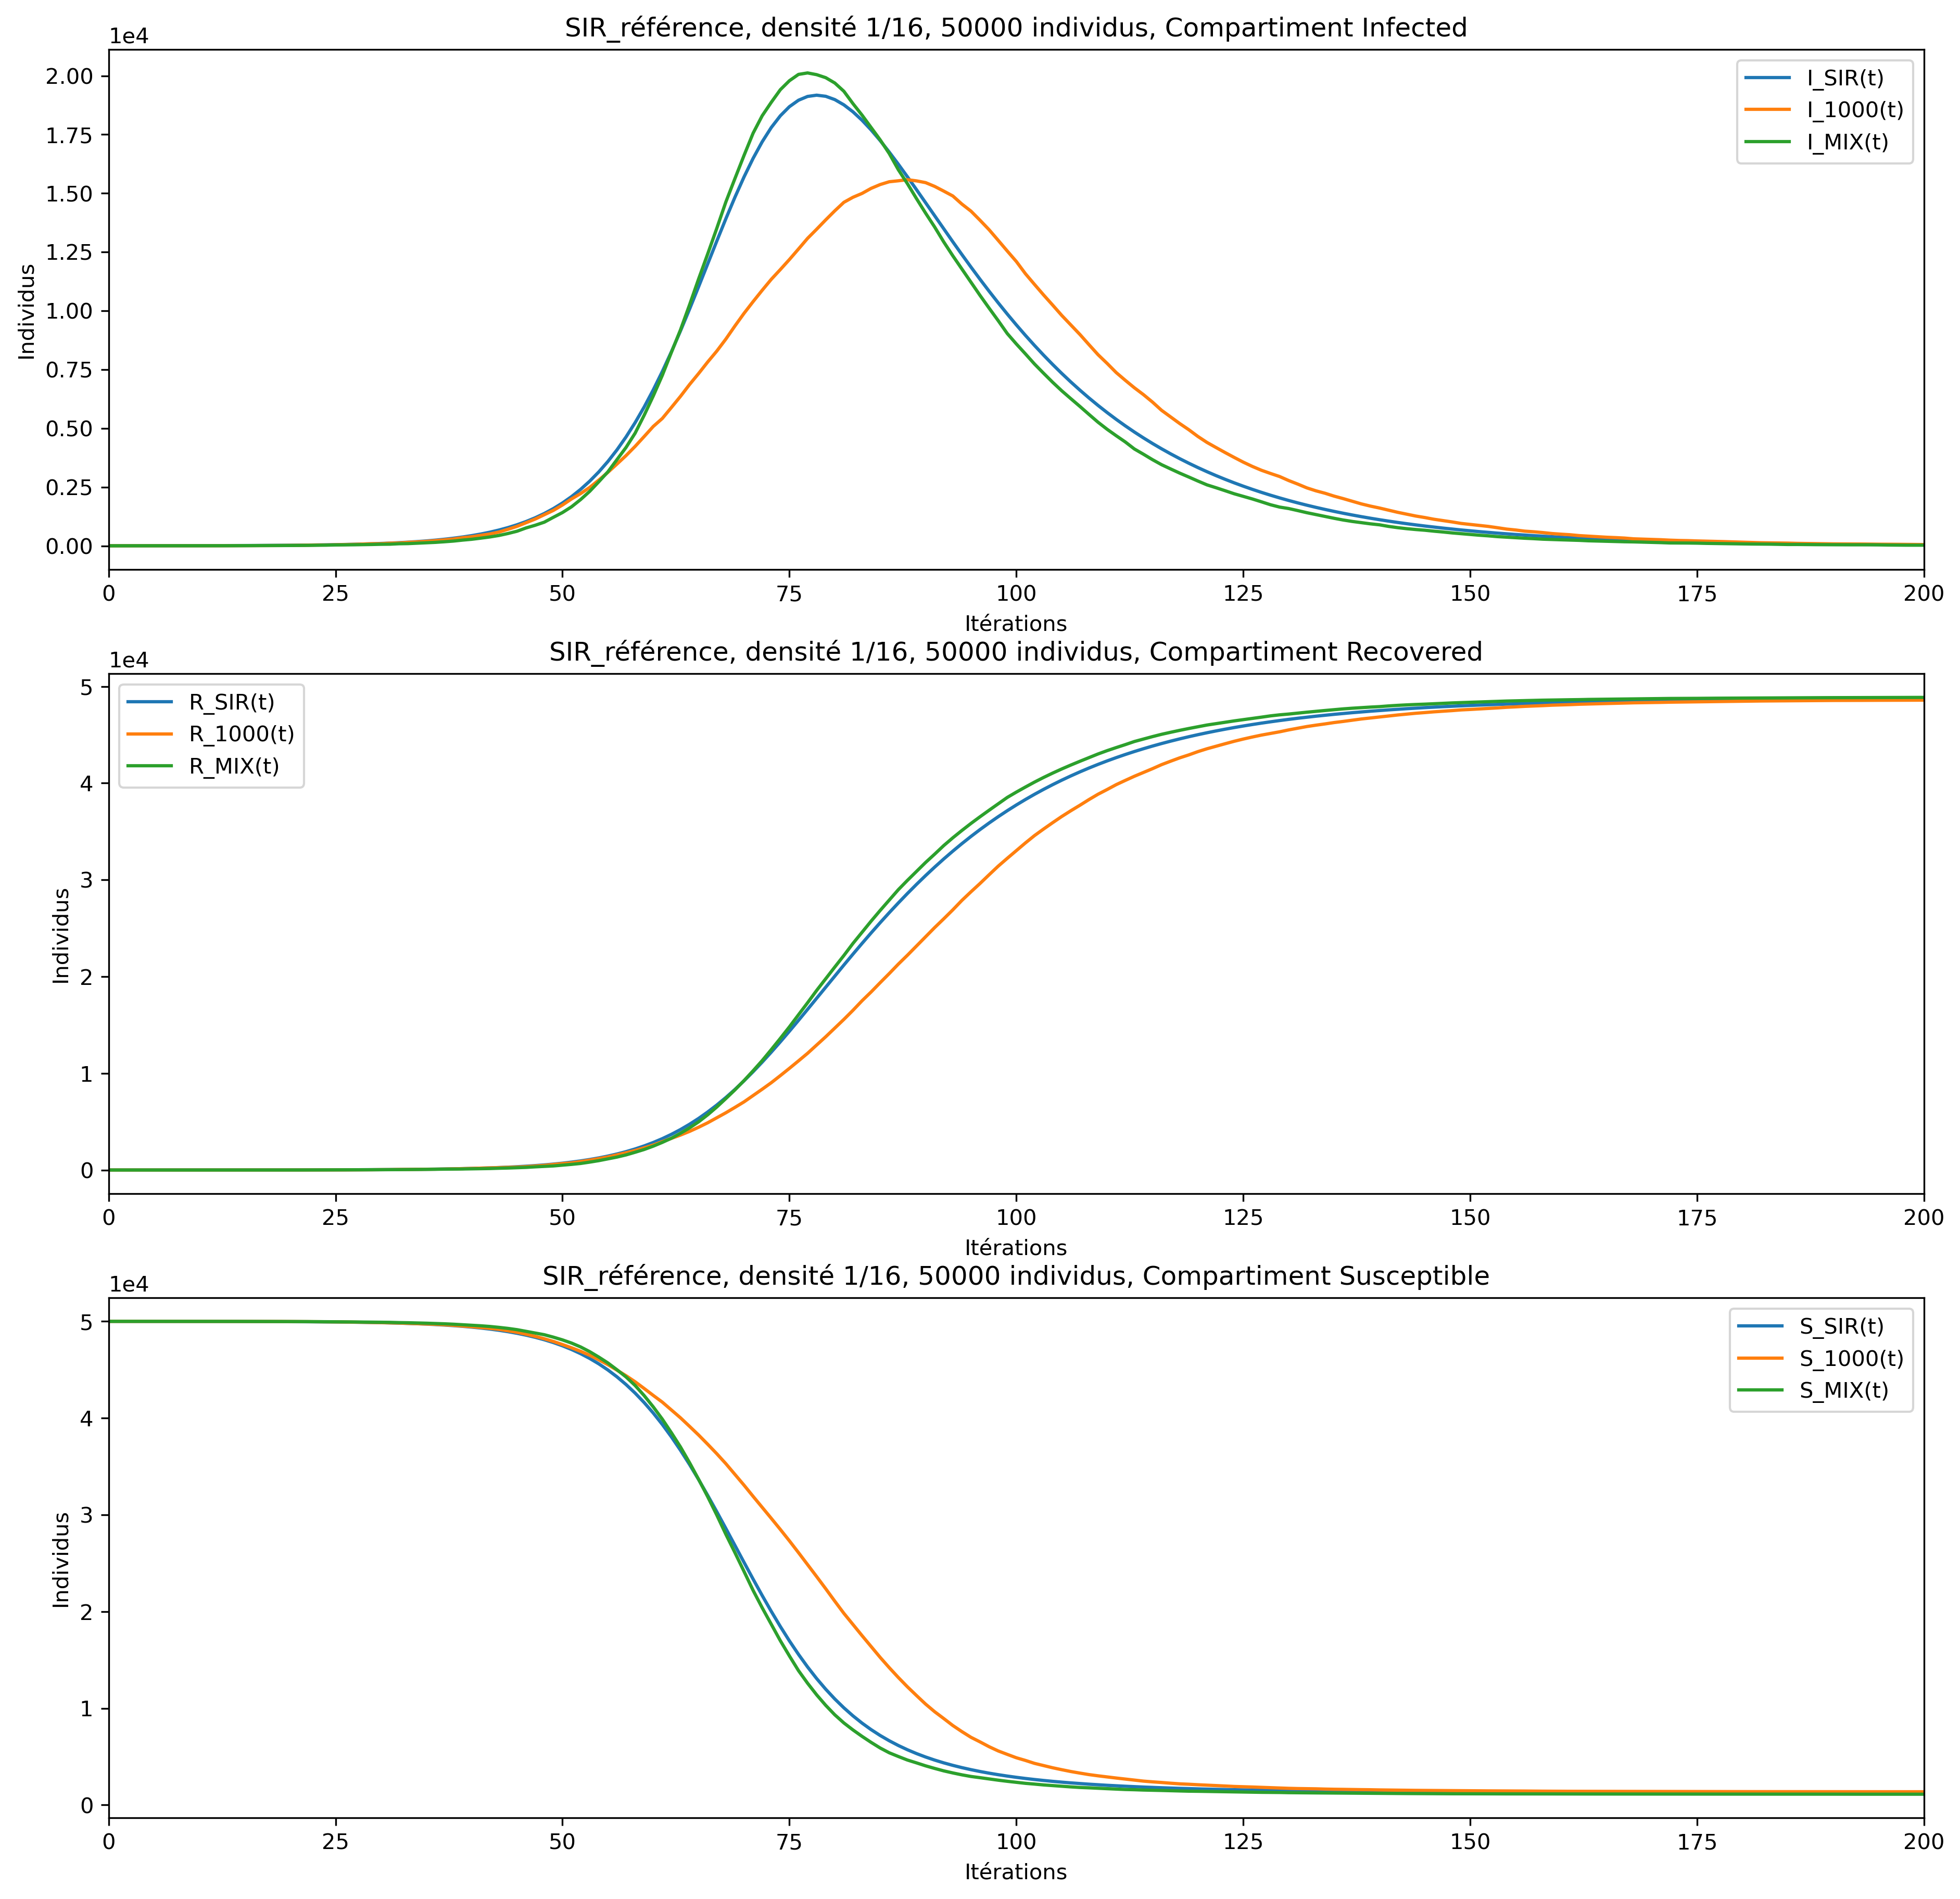
\includegraphics[width=.4\textwidth]{Images/SIR_ref_16_50.png}
	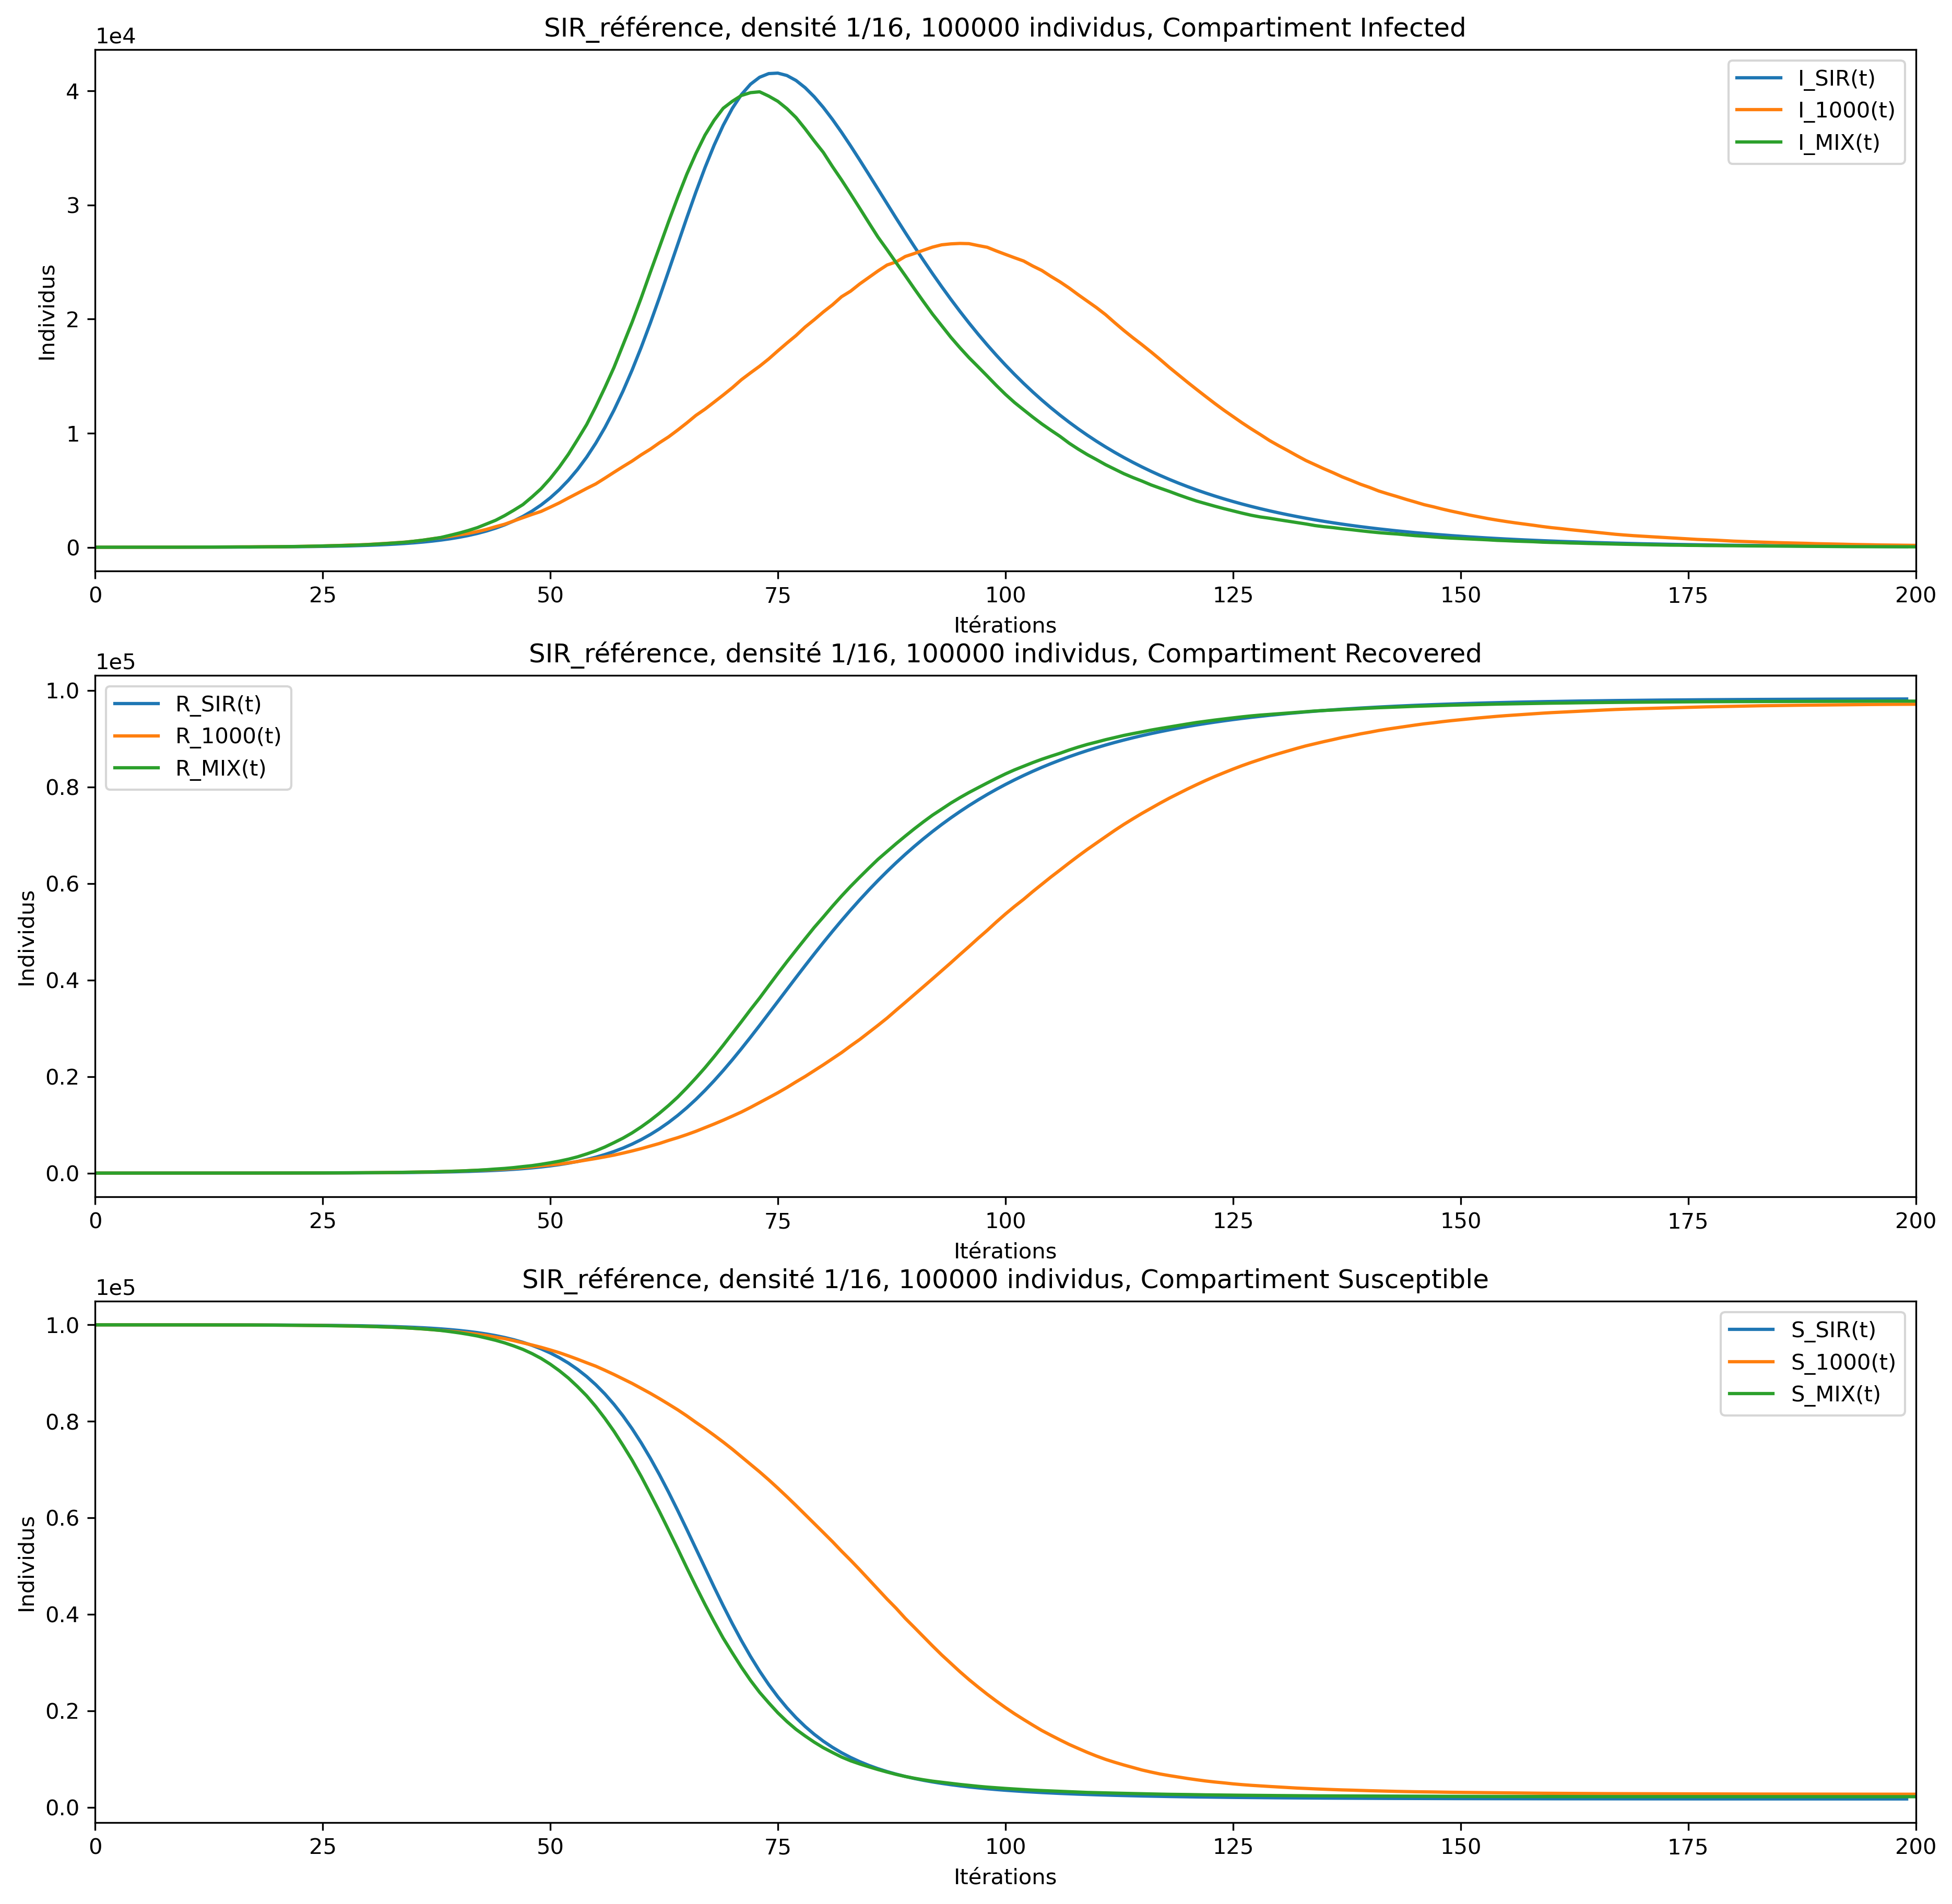
\includegraphics[width=.4\textwidth]{Images/SIR_ref_16_100.png}
	\caption{test}
\end{figure}

Tout comme pour le modèle SI, les simulations aux $1000$ mouvements sont ralenties par les systèmes de grande taille car le mouvement des individus est réduit par rapport à la taille du système. C'est la raison pour laquelle les courbes au $1000$ mouvements sont retardées.\\

Malgré des observations déjà analysées, nous obsevons des oscillations sur la simulation à $5000$ indiviuds. Ce phénomène n'était pas présent sur les simulations SI et ceci à cause de l'absense du compartiment $Recovered$. Deux raisons explique ce comportement, le premier est que le mécanisme d'immunisation transfert des individus du compartiment $I$ au $R$ et donc abaisse la courbe. Le second est dû à la densité du système qui est très faible, par conséquent il y a peu de contactes qui s'effectuent ce qui crée des oscillations. Ces oscillations sont aussi présentes sur des sytèmes plus denses mais pas perceptibles car moyennée par un grand nombre d'événements.

\section{Analyses}

\subsection{Mean Absolute Error}

\begin{table}[H]
	\centering
	\captionsetup{justification=centering}
	\caption[Mean Aboslute Error Normalized : SI]{Mean Aboslute Error Normalized : modèle SIR, mélange parfait \label{tab:grid}}
	\begin{tabular}{@{\extracolsep{\fill} } c|| c| c| c| c|}
	 & 5000 & 20000 & 50000 & 100000\\ 
	\midrule
	\midrule
	1/2 & $4.3\mathrm{e}{-3}$ & $2.1\mathrm{e}{-3}$ & $2.7\mathrm{e}{-3}$ & $2.5\mathrm{e}{-3}$\\
	\midrule
	1/4 & $3.8\mathrm{e}{-3}$ & $3.0\mathrm{e}{-3}$ & $2.1\mathrm{e}{-3}$ & $2.6\mathrm{e}{-3}$\\
	\midrule
	1/8 & $9.6\mathrm{e}{-3}$ & $2.8\mathrm{e}{-3}$ & $1.9\mathrm{e}{-3}$ & $2.3\mathrm{e}{-3}$\\
	\midrule
	1/16 & $8.5\mathrm{e}{-3}$ & $3.2\mathrm{e}{-3}$ & $6.2\mathrm{e}{-3}$ & $7.2\mathrm{e}{-3}$\\
	\bottomrule
	\end{tabular}
	\end{table}

\subsection{Positions des individus}

plot pour le mélange parfait

\begin{figure}[h]
	\centering
	\captionsetup{justification=centering}
	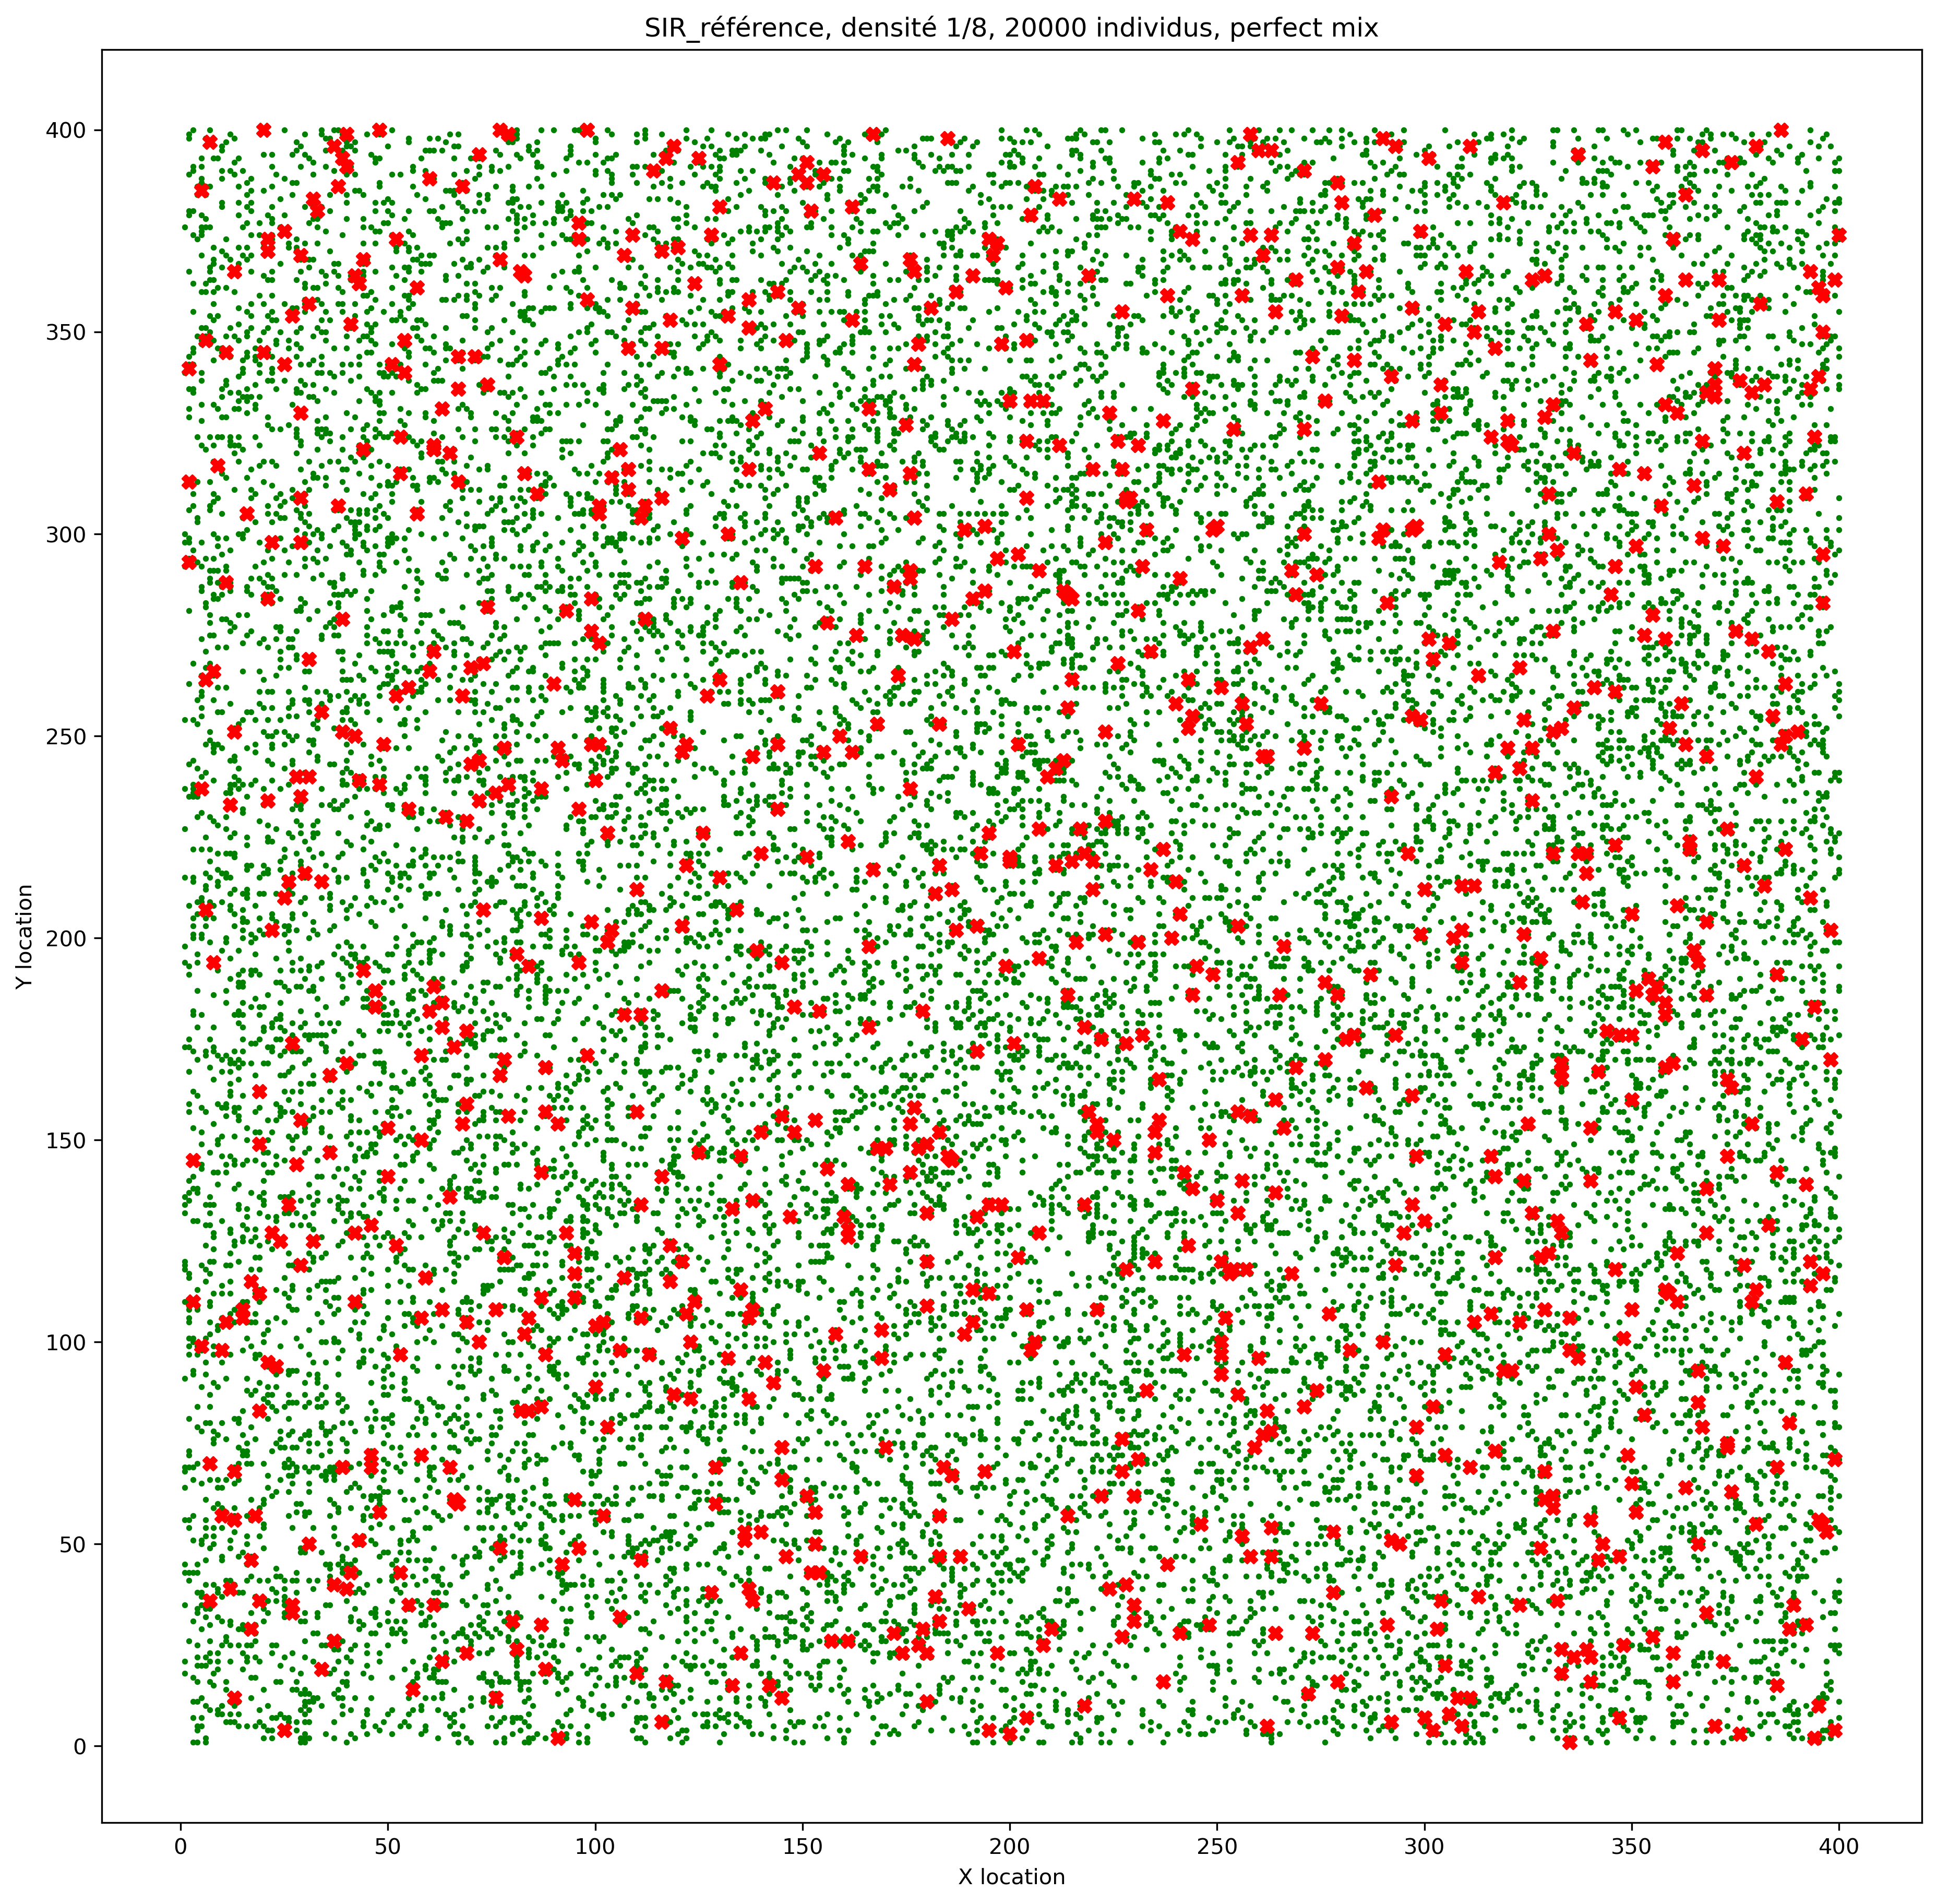
\includegraphics[width=.7\textwidth]{Images/SIR_position_8_20_perfect_mix.png}
	\caption{test}
\end{figure}

explications

\newpage

\begin{figure}[h]
	\centering
	\captionsetup{justification=centering}
	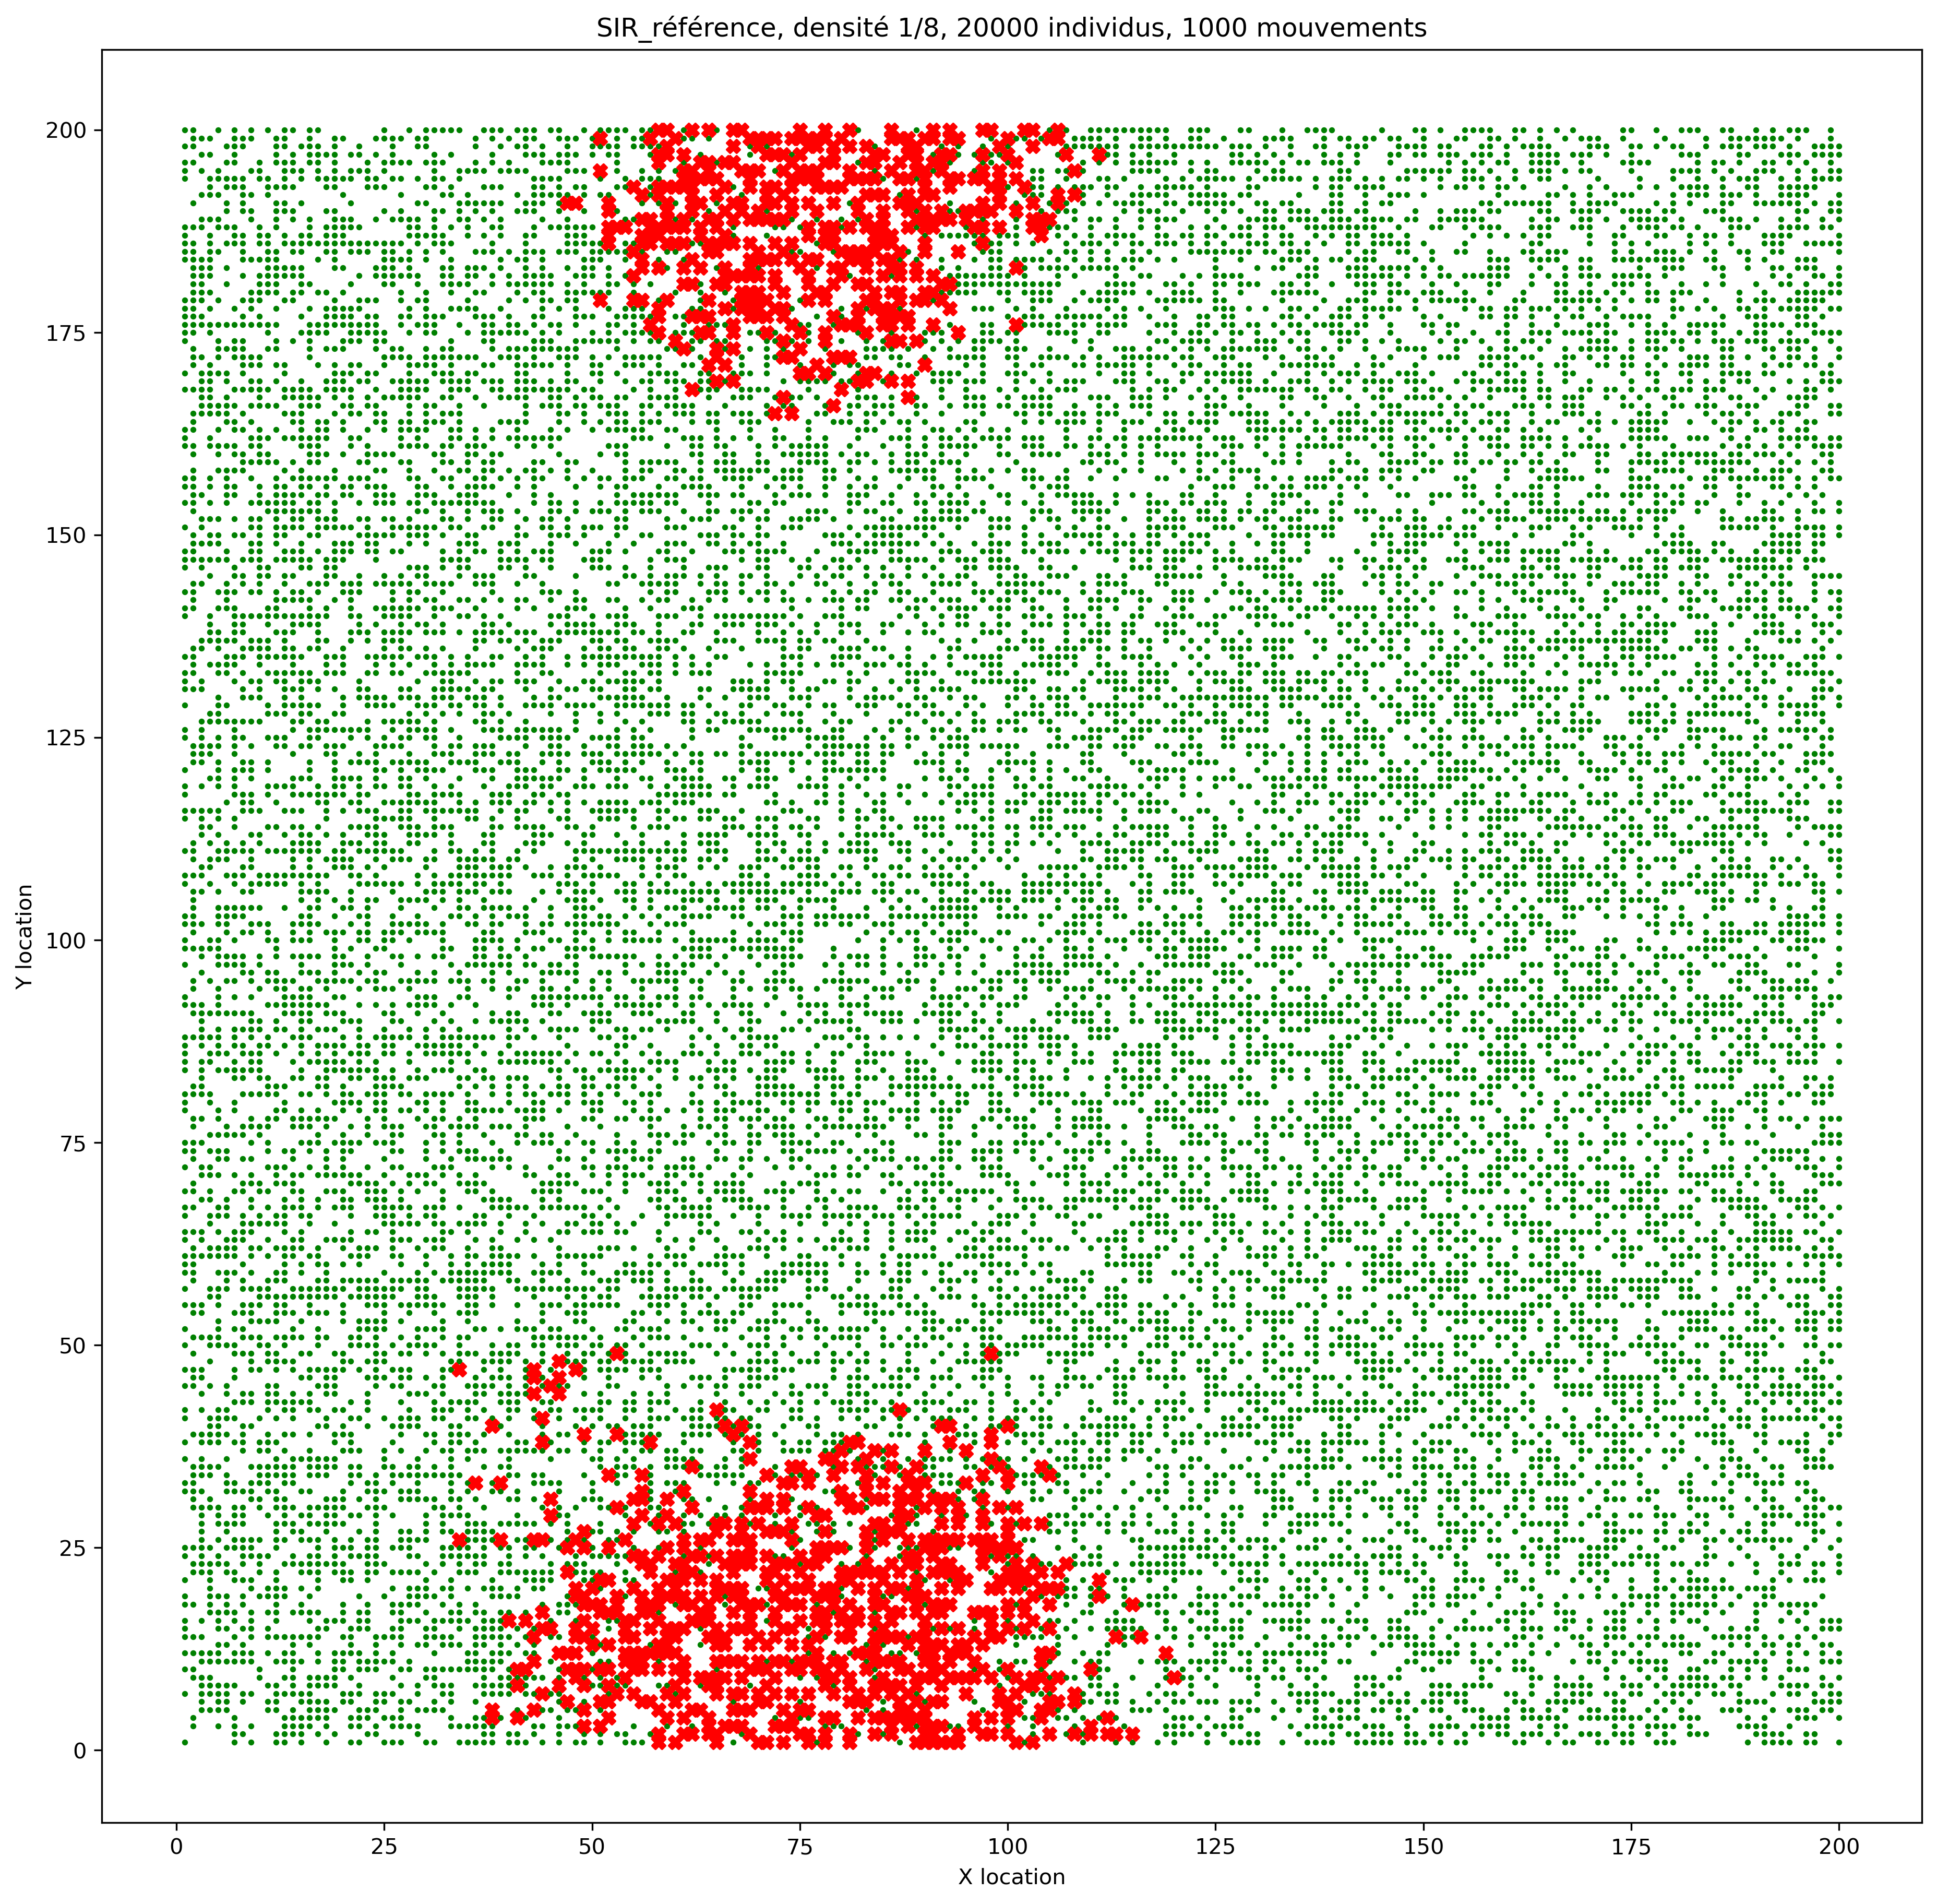
\includegraphics[width=.4\textwidth]{Images/SIR_position_2_20.png}
	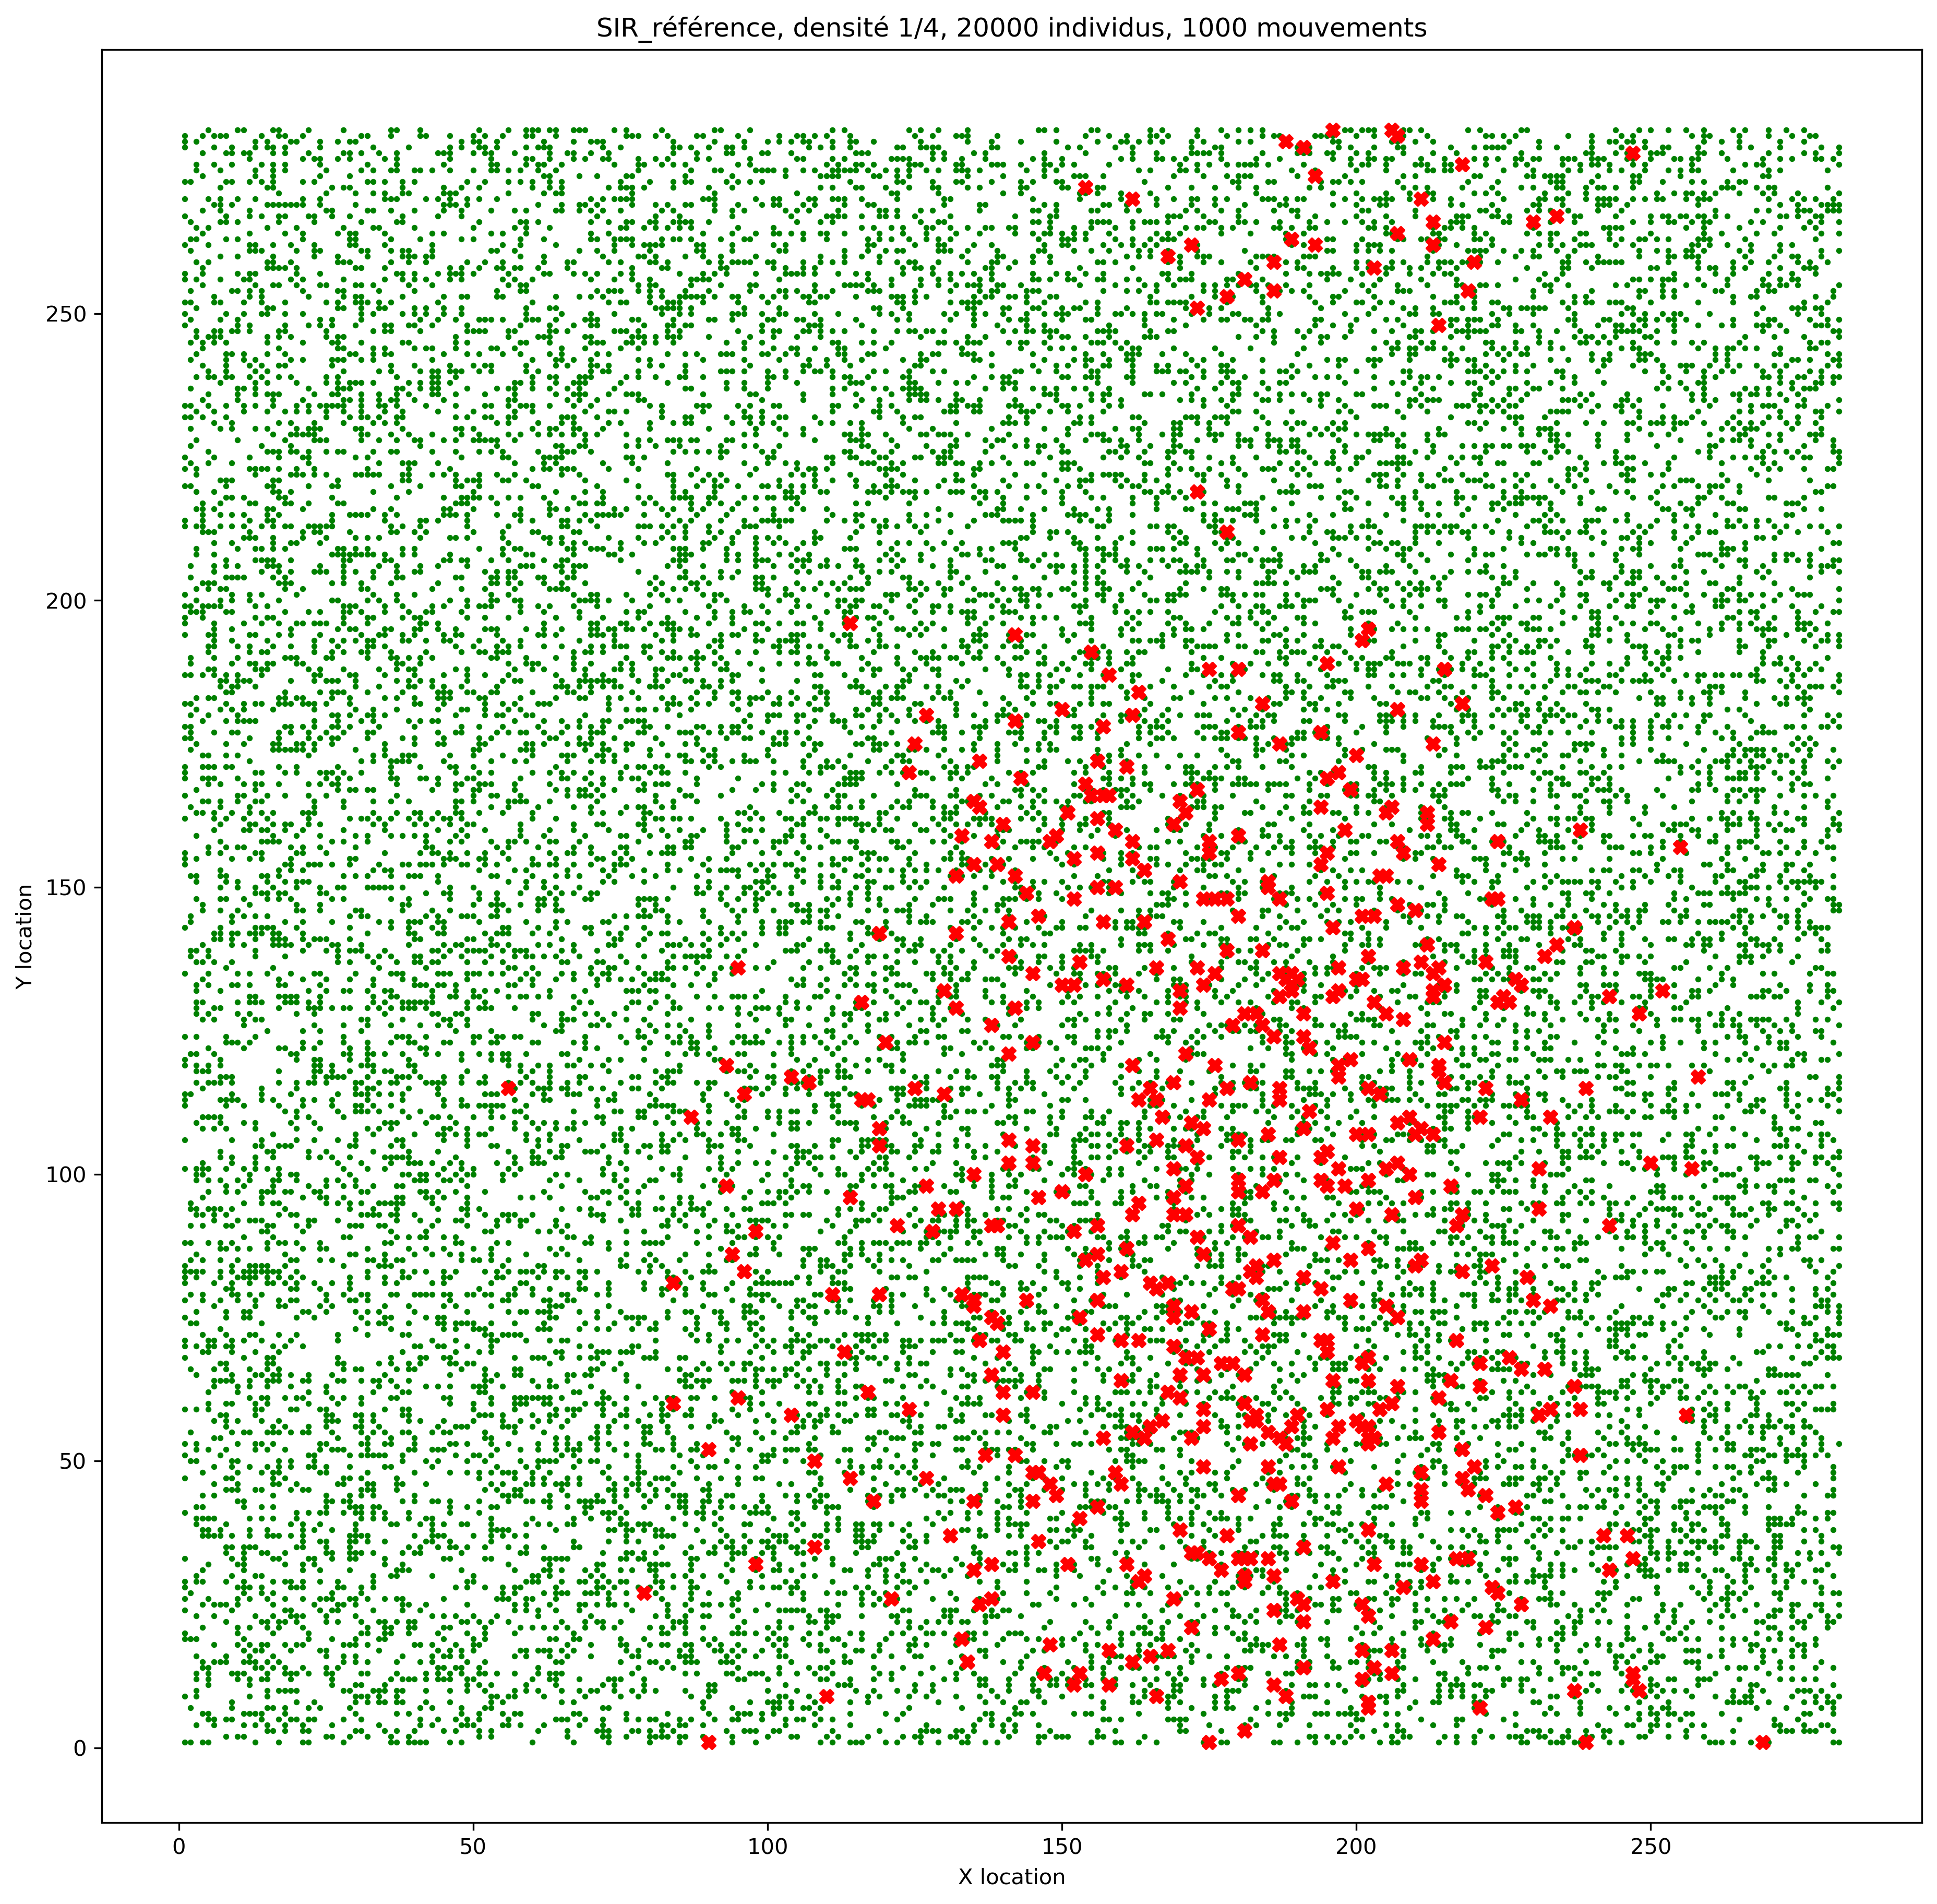
\includegraphics[width=.4\textwidth]{Images/SIR_position_4_20.png}
	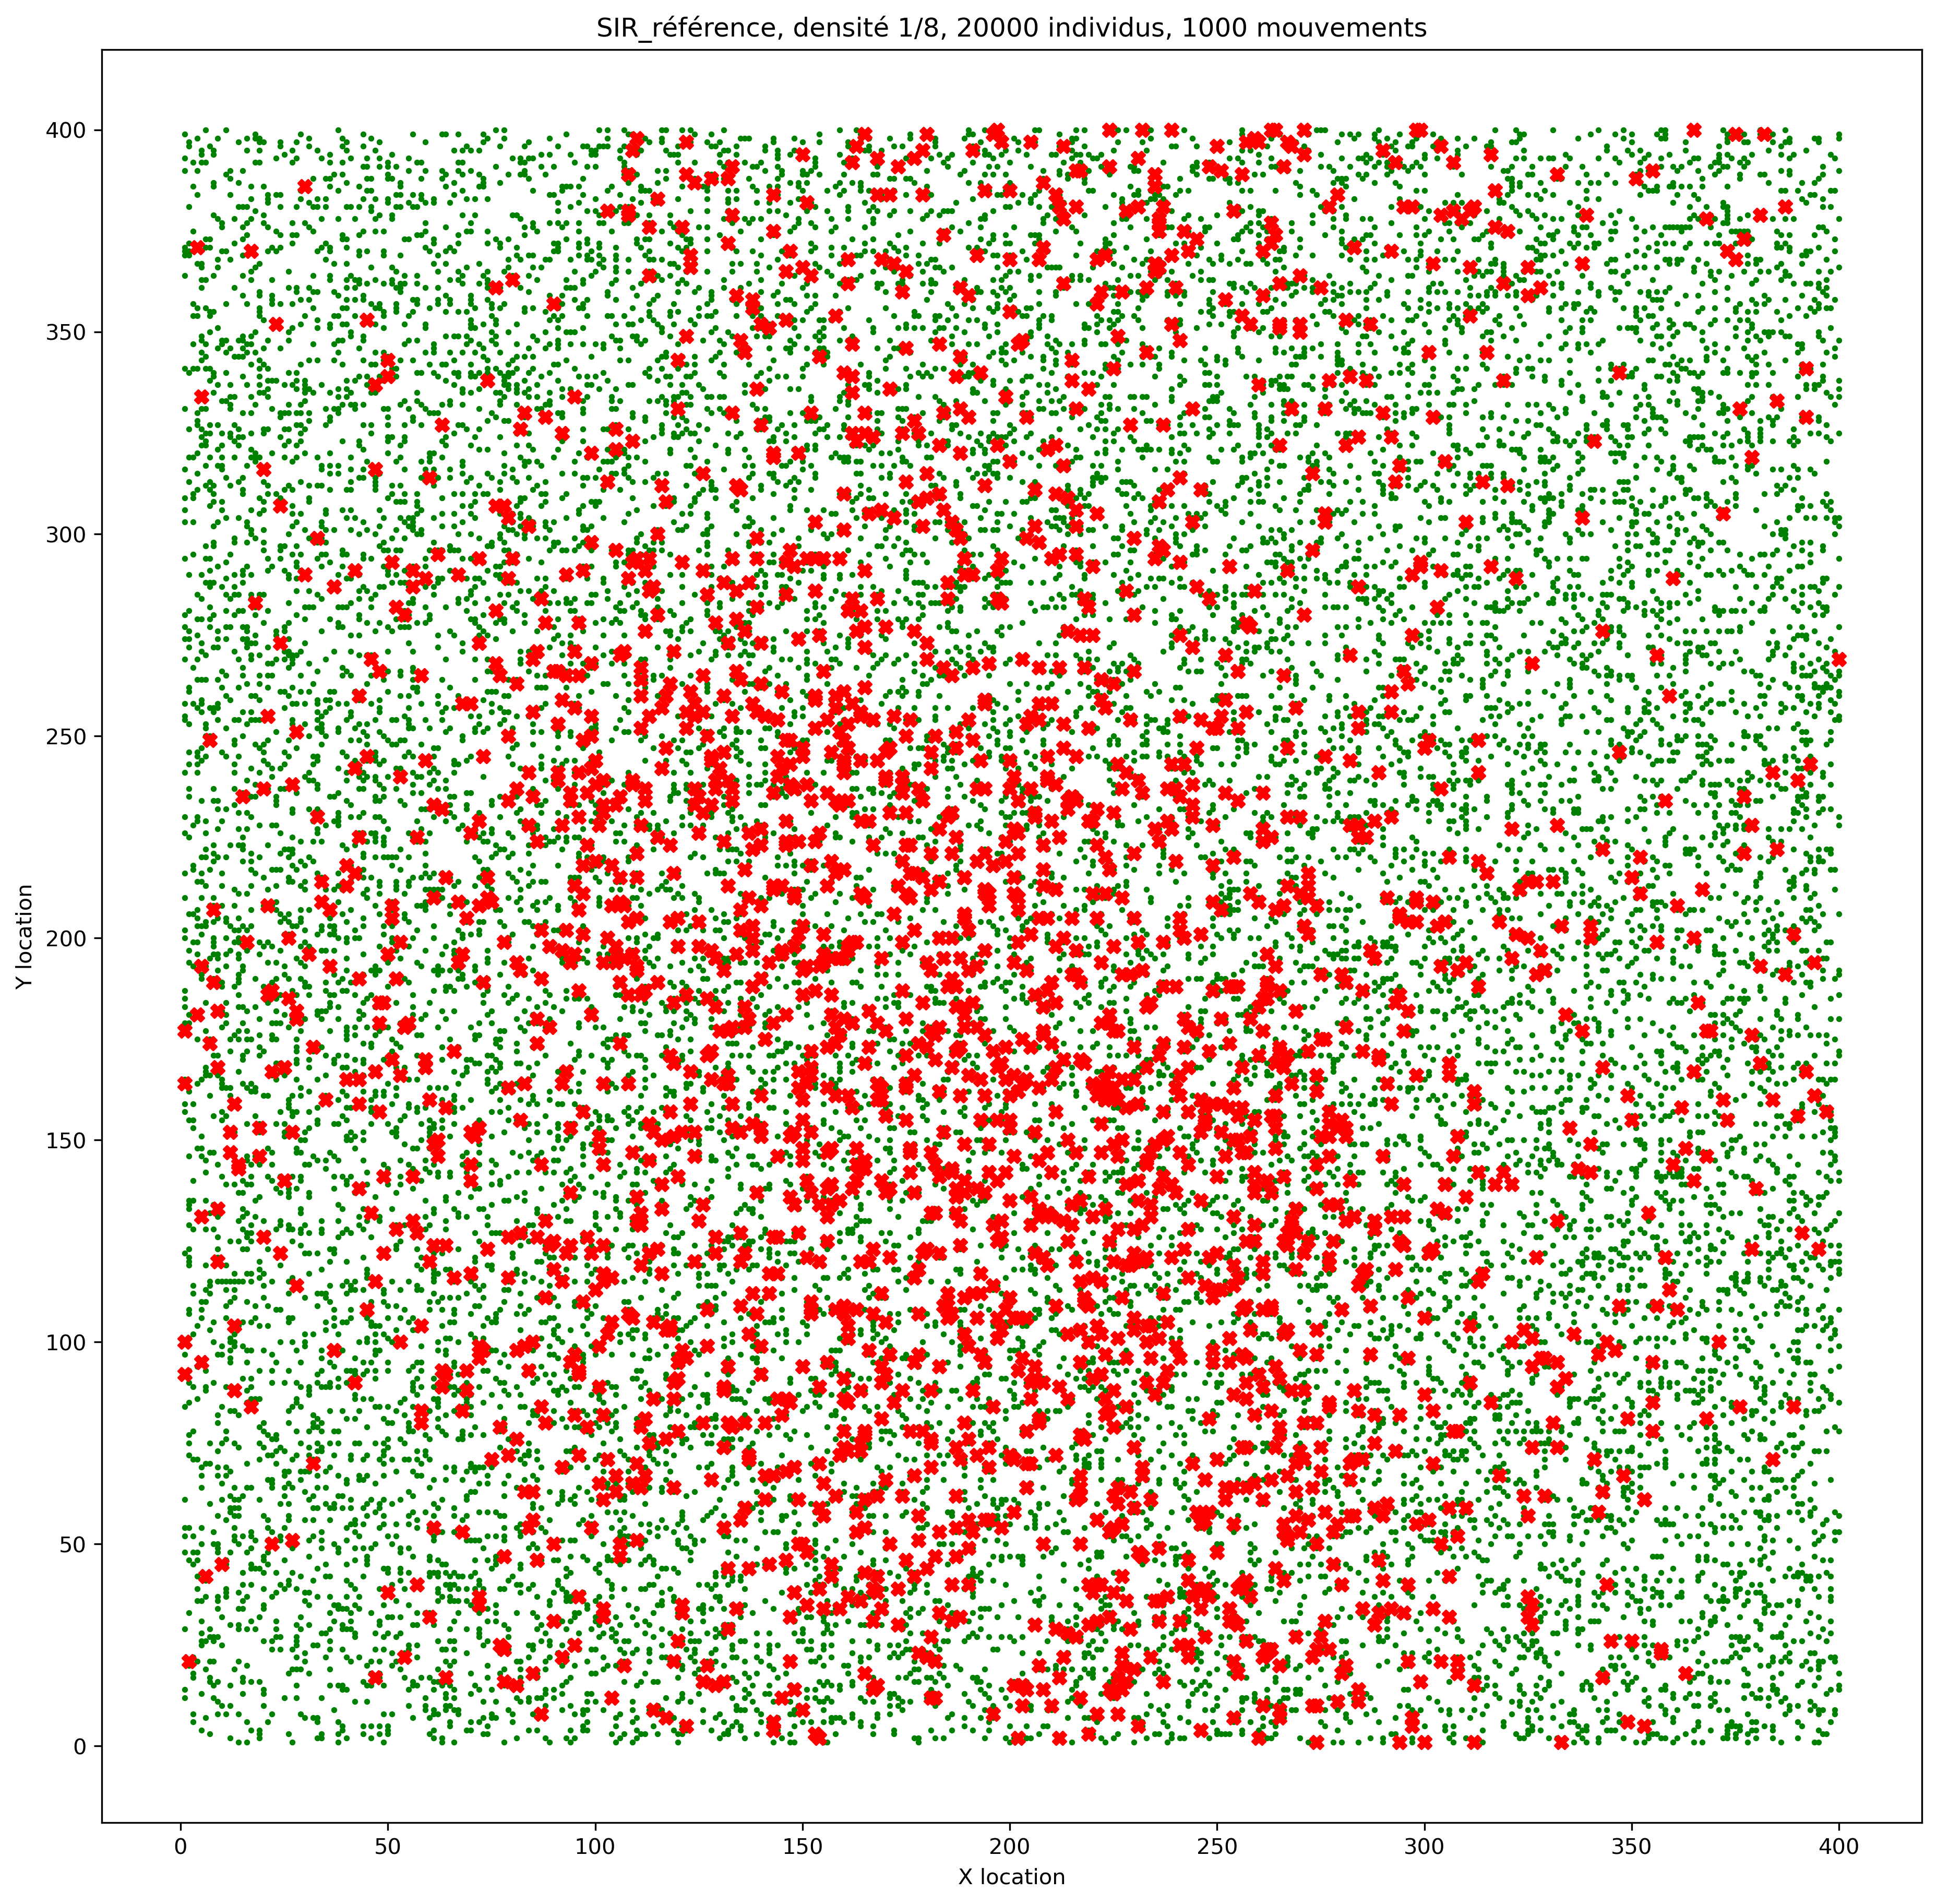
\includegraphics[width=.4\textwidth]{Images/SIR_position_8_20.png}
	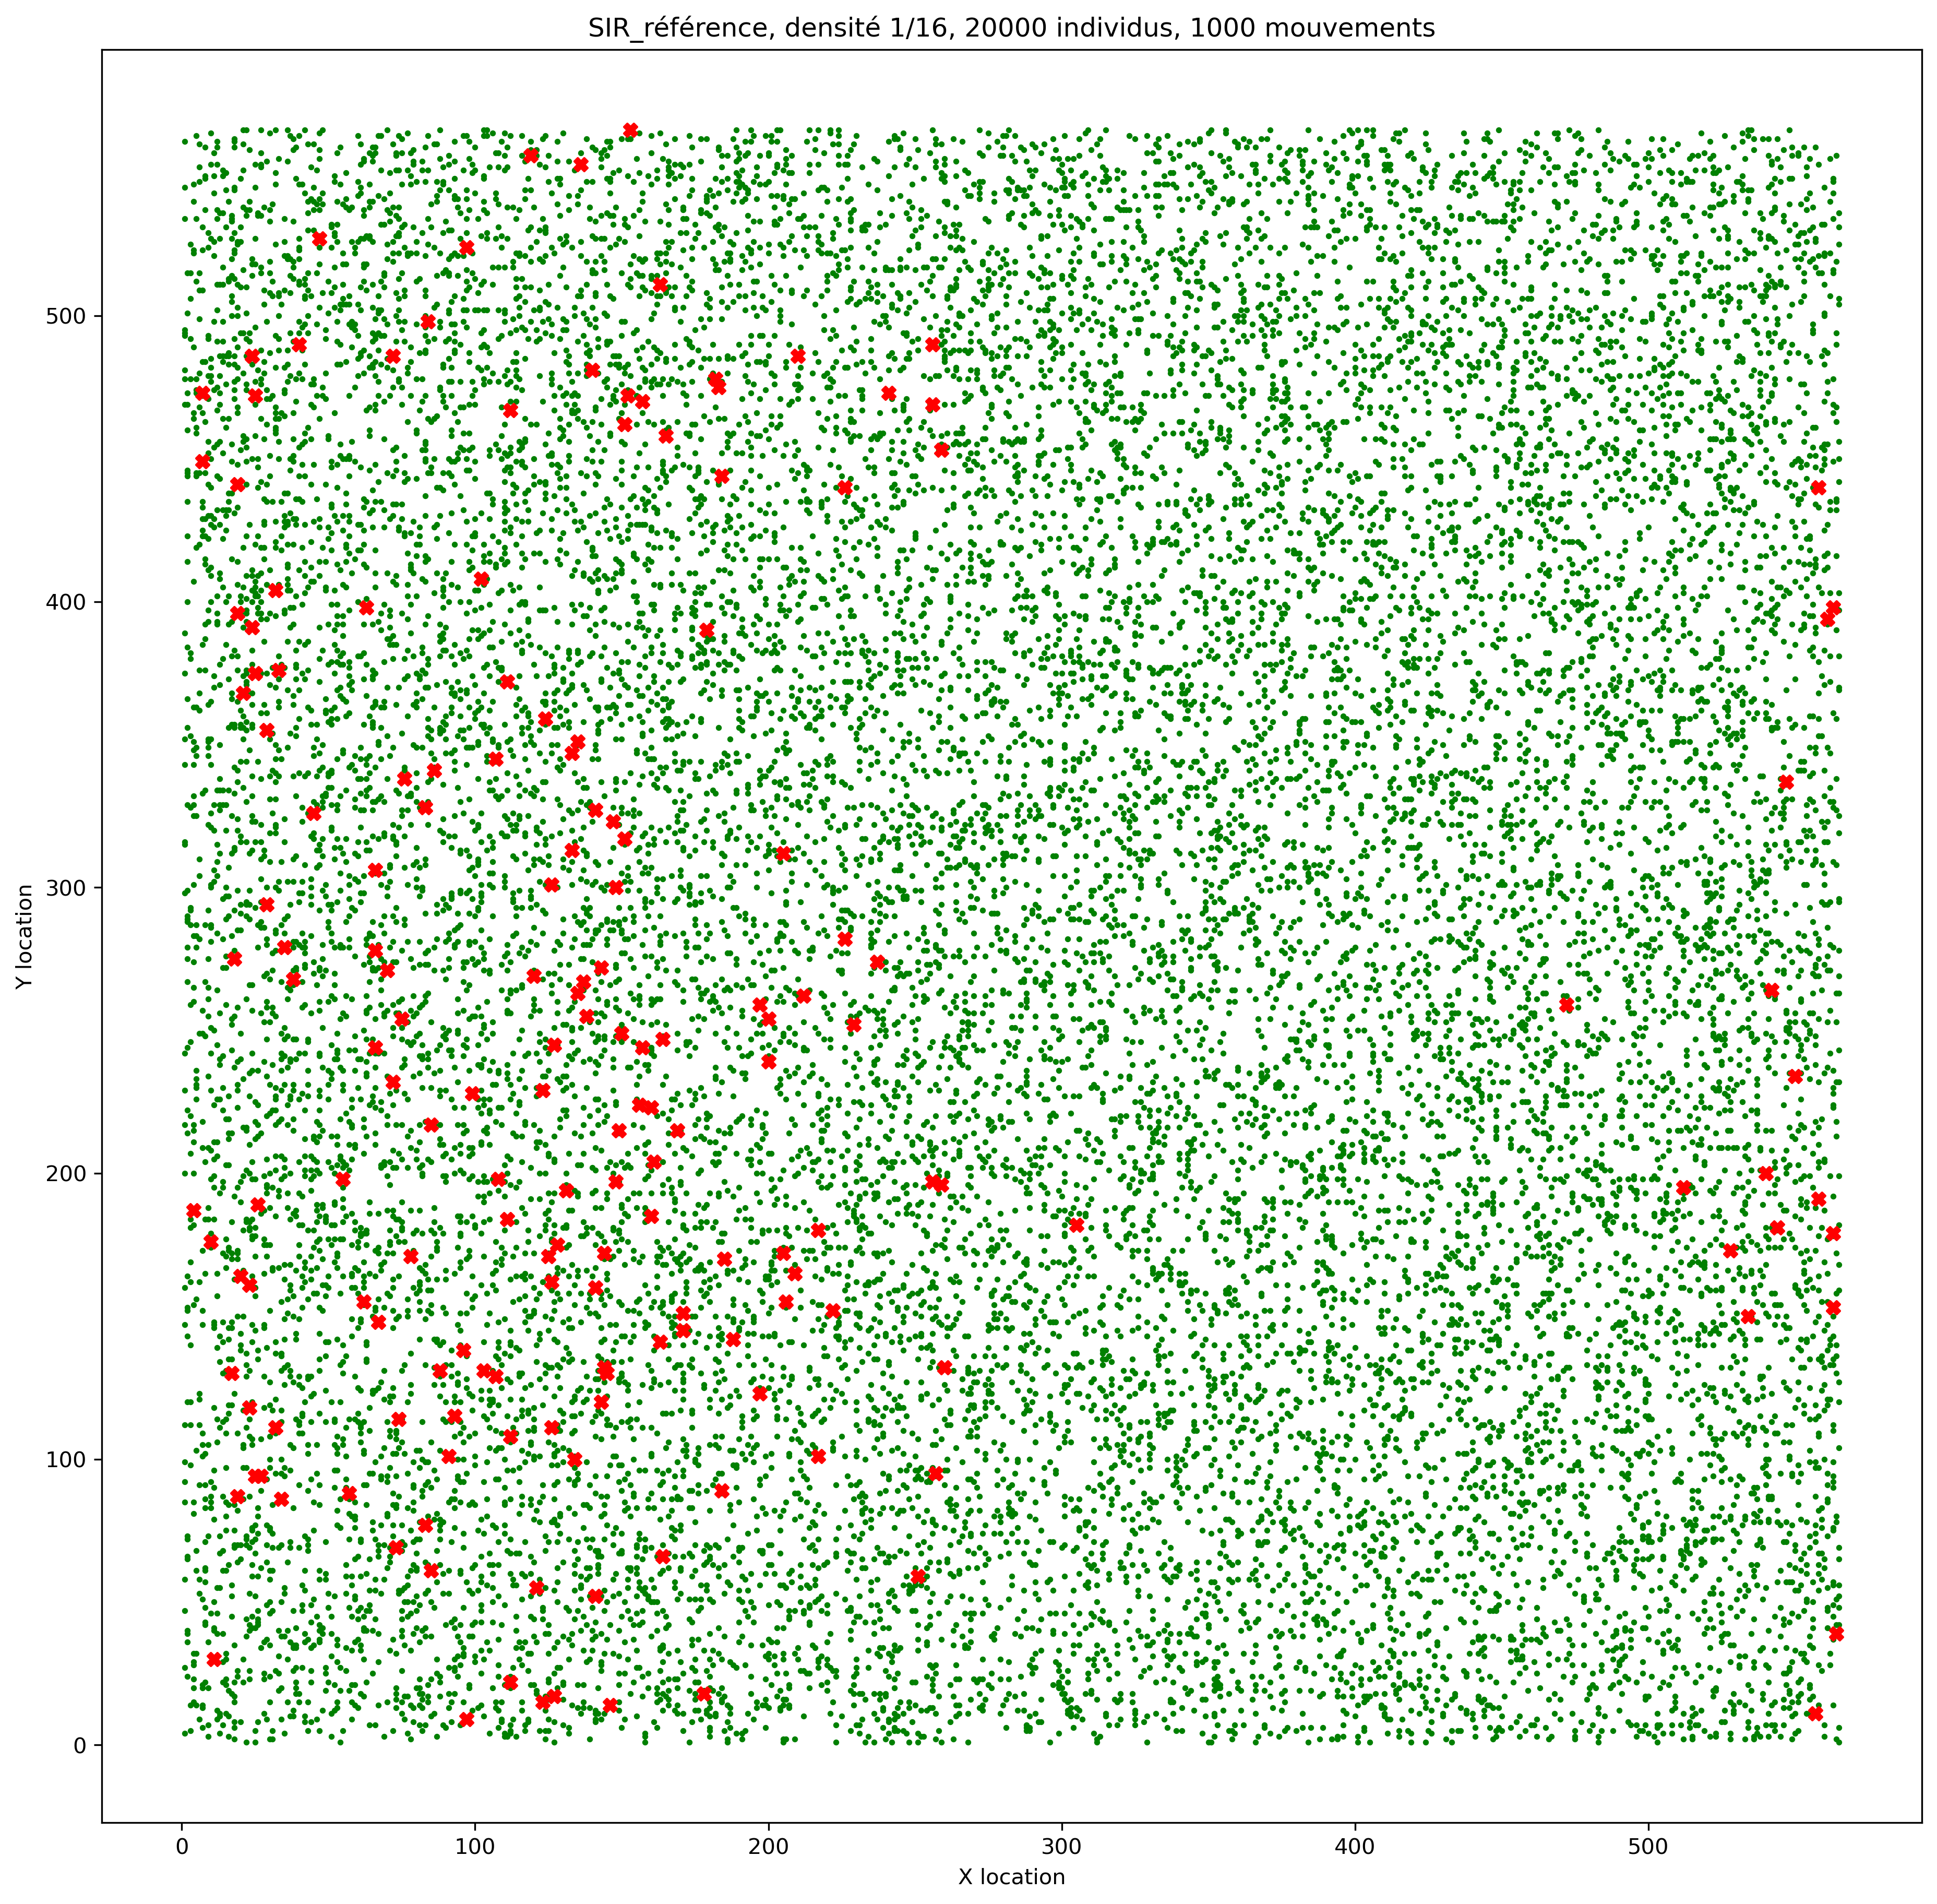
\includegraphics[width=.4\textwidth]{Images/SIR_position_16_20.png}
	\caption{test}
\end{figure}

explications

\newpage

\subsection{Variations aléatoires}

\begin{wrapfigure}{r}{0.5\textwidth}
    \centering
    \captionsetup{justification=centering}
    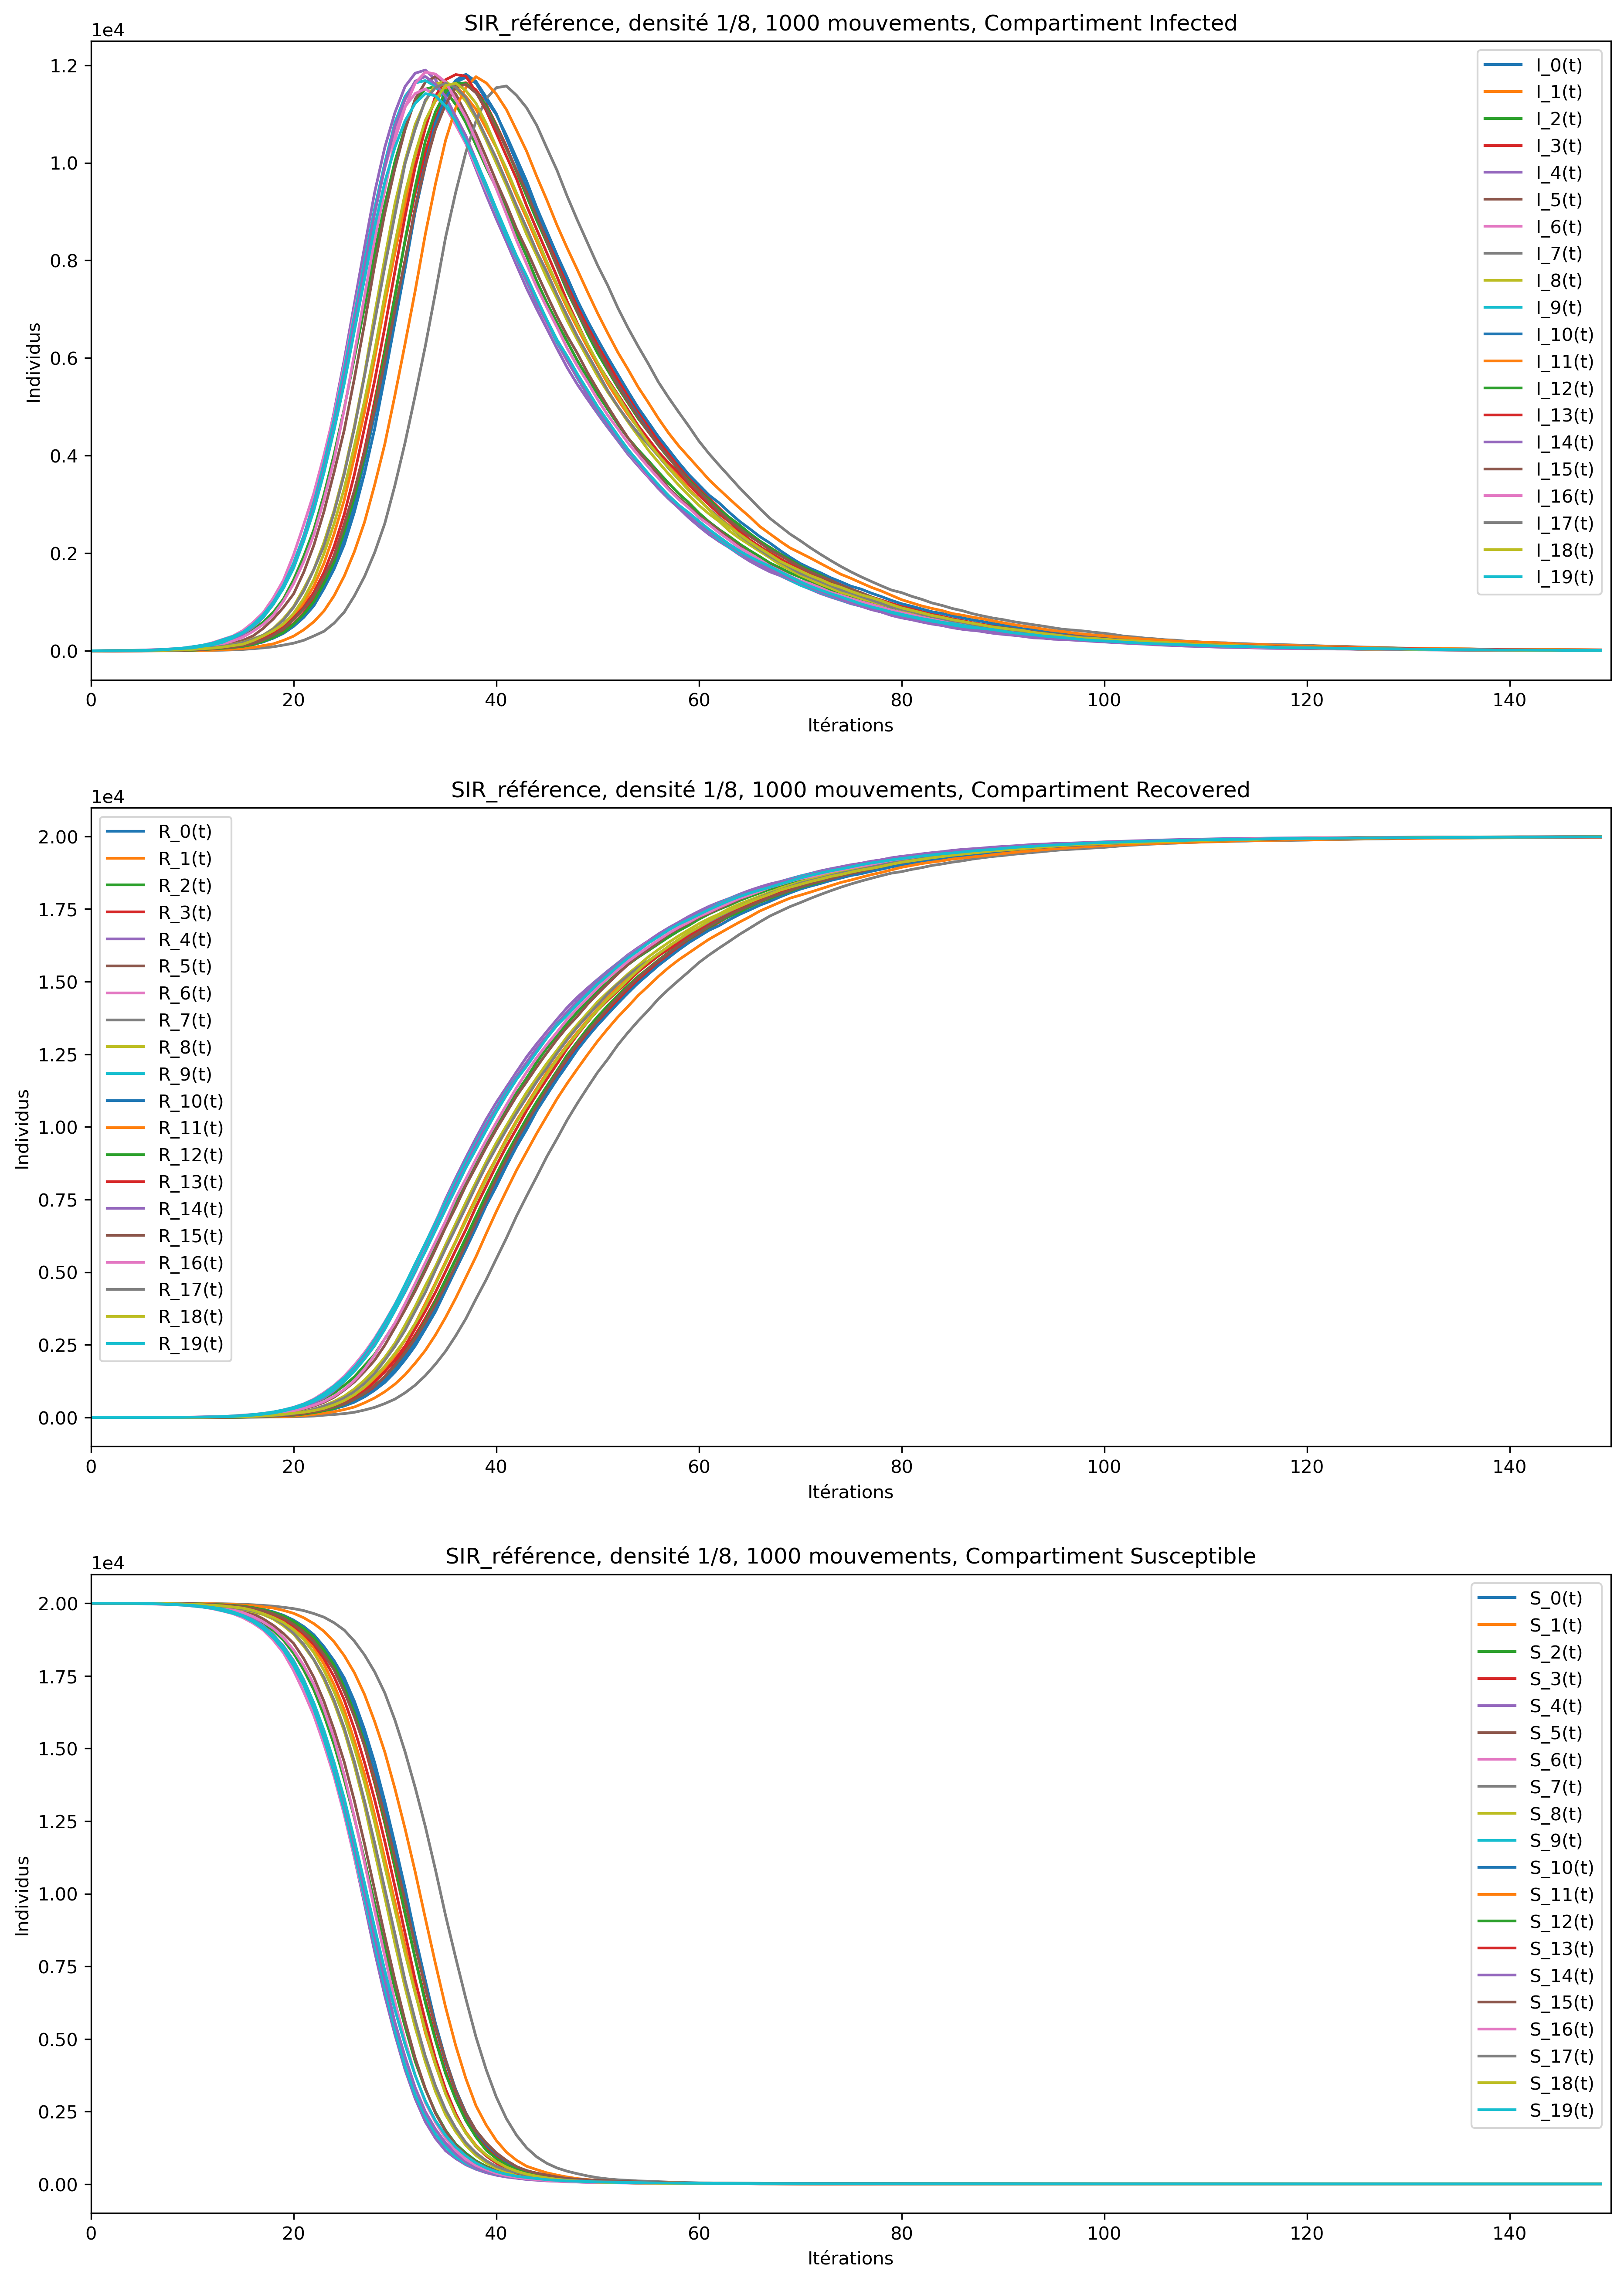
\includegraphics[width=0.5\textwidth]{Images/SIR_divergence_8_1000.png}
    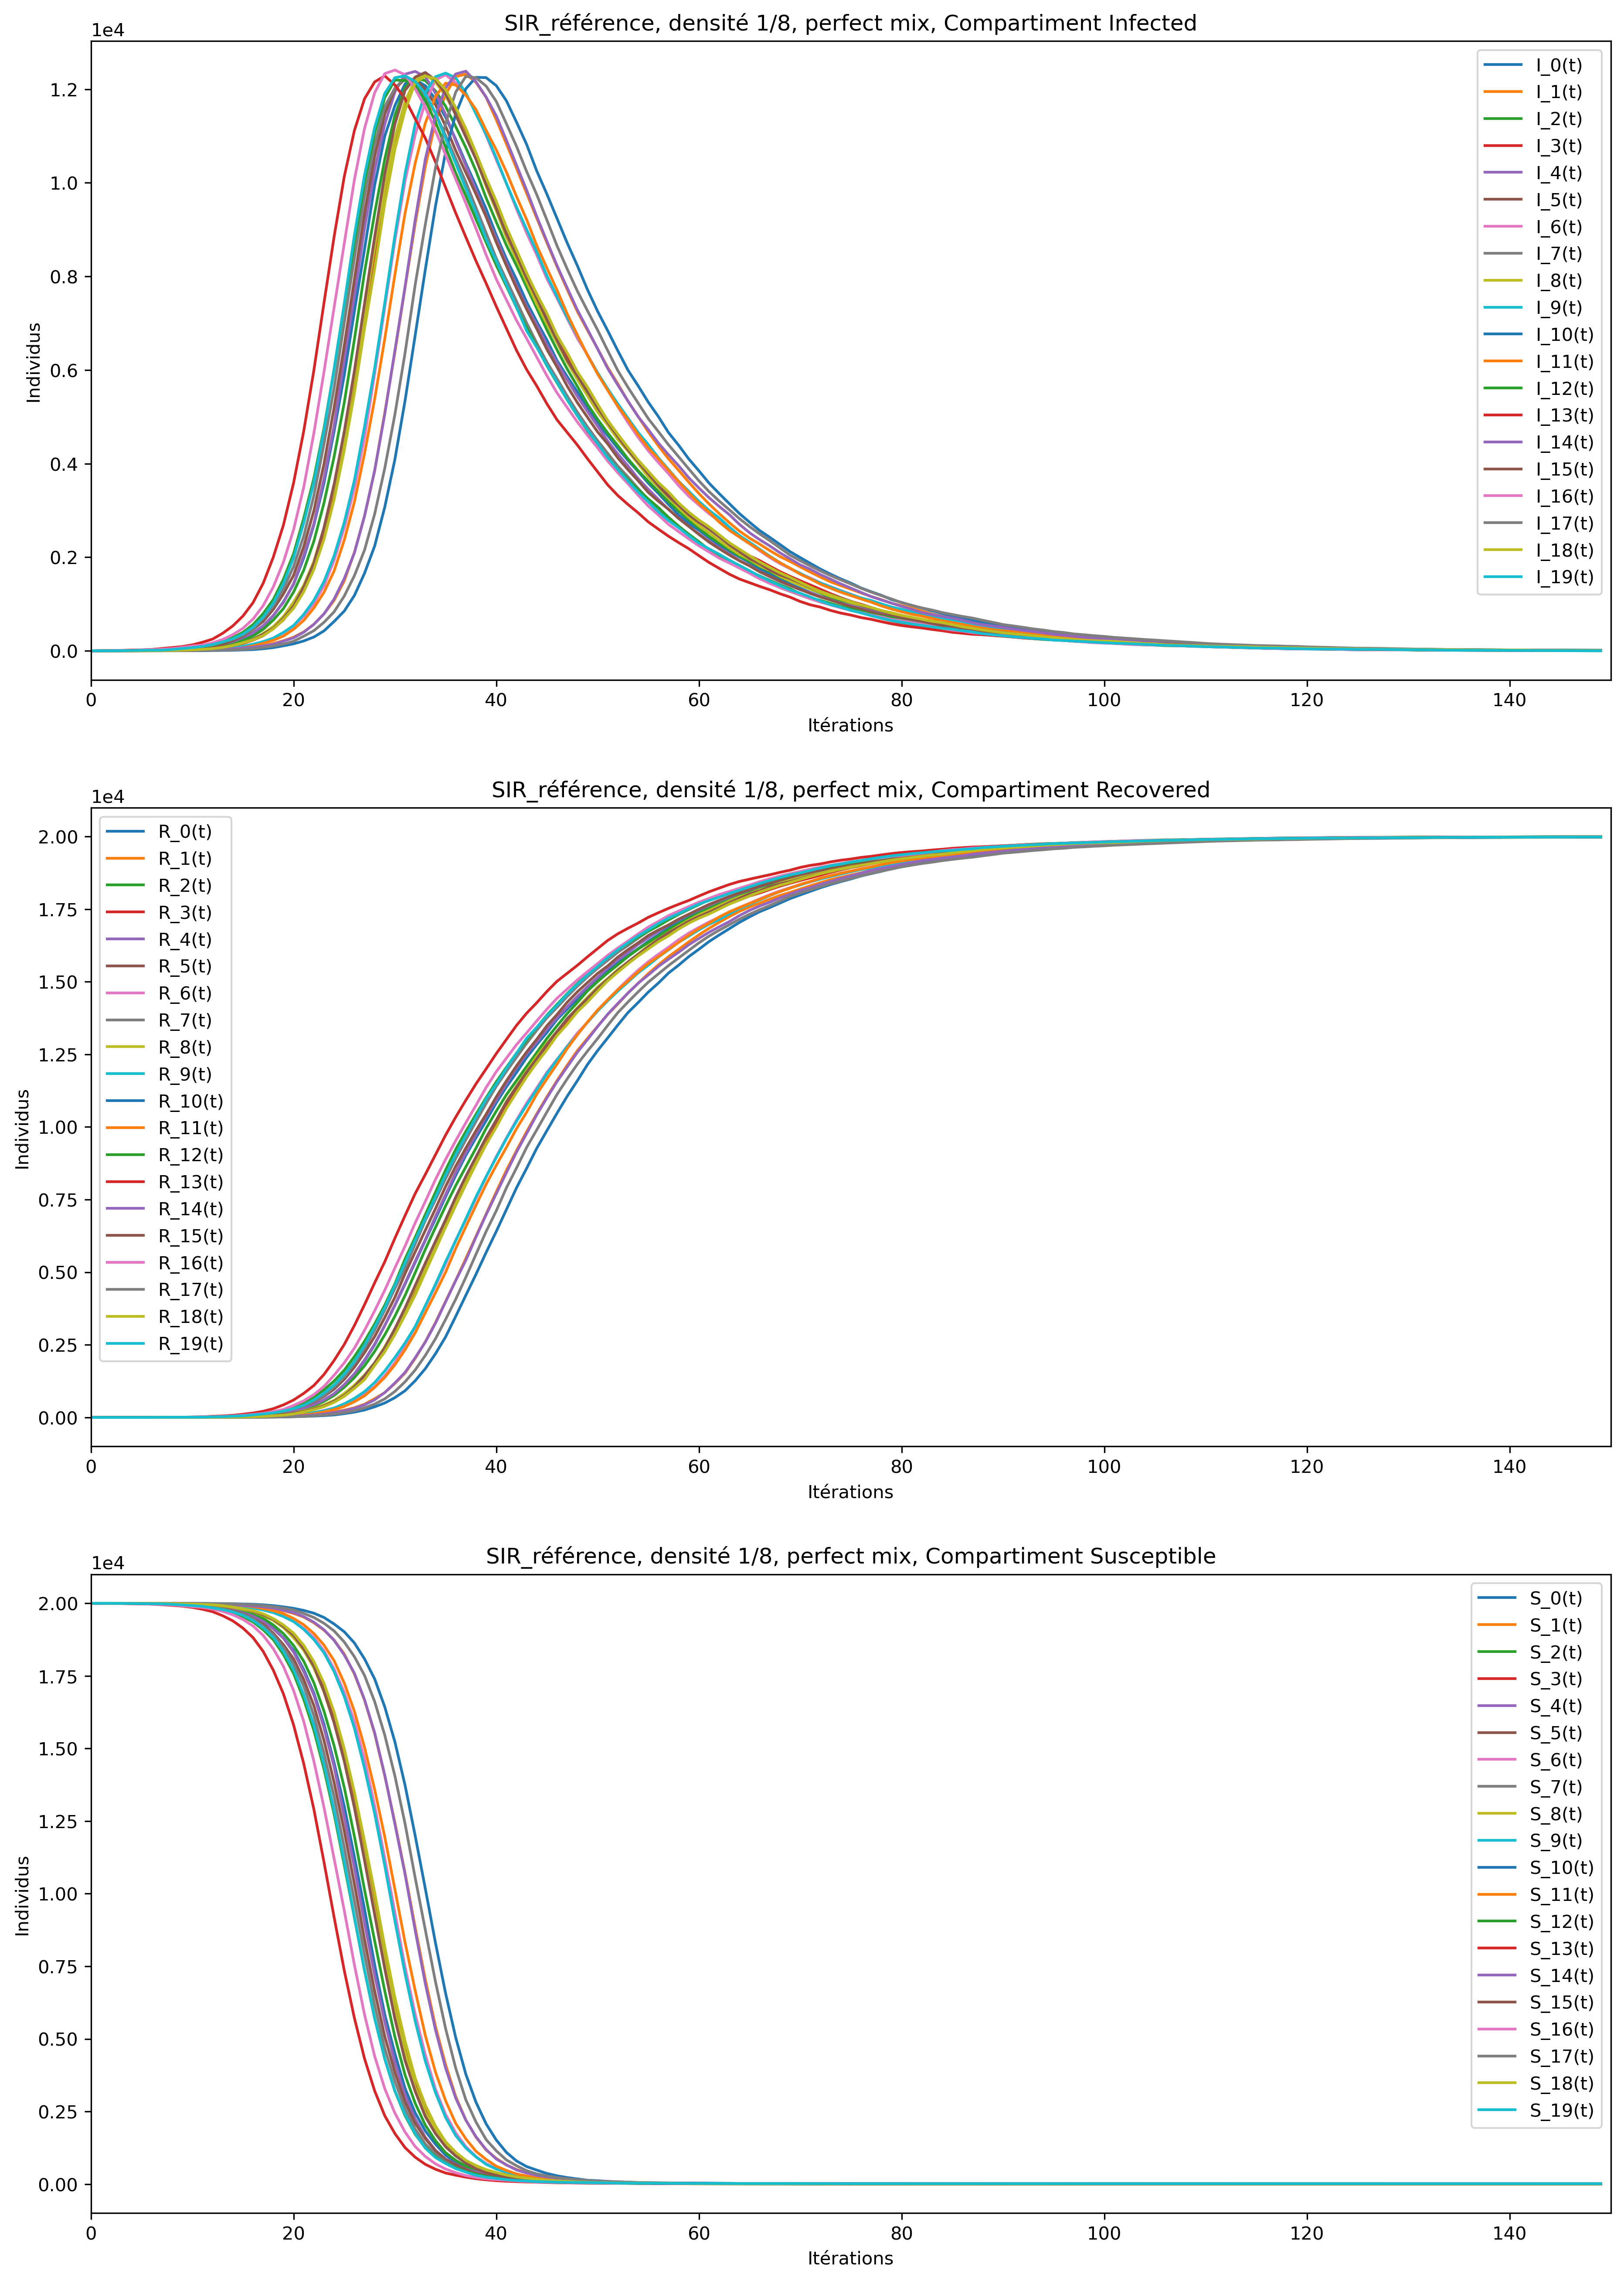
\includegraphics[width=0.5\textwidth]{Images/SIR_divergence_8_mix.png}
    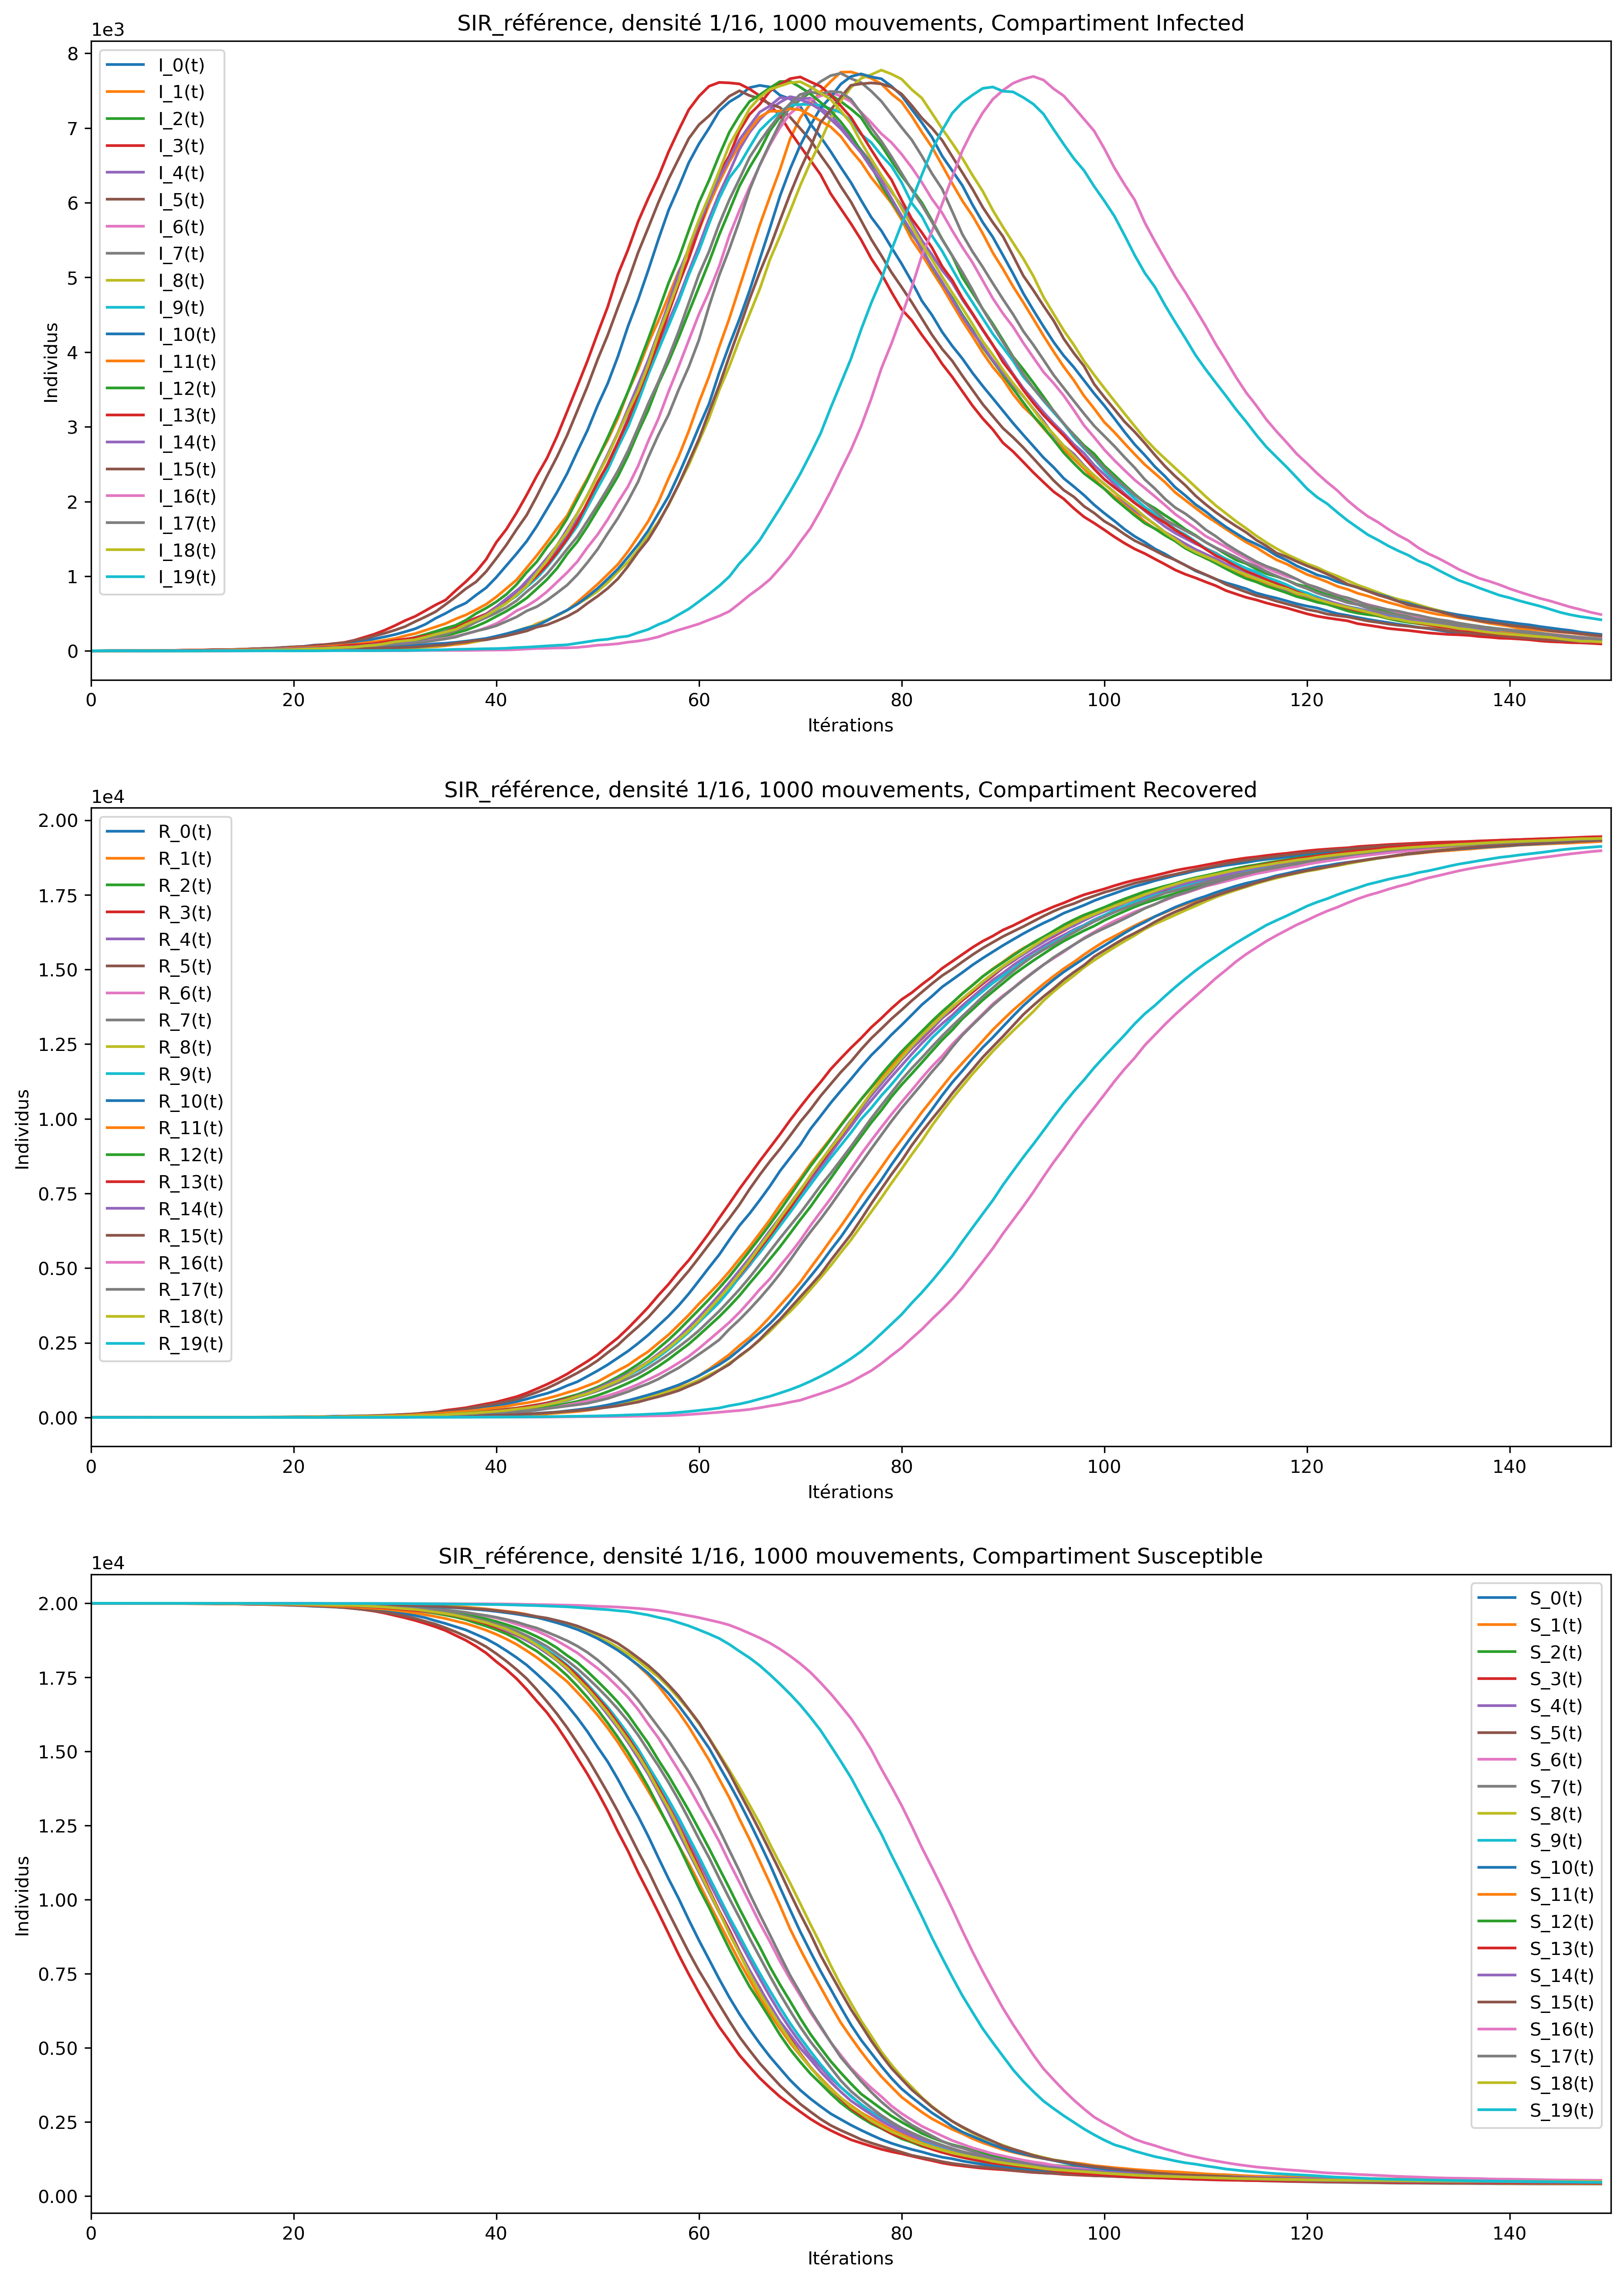
\includegraphics[width=0.5\textwidth]{Images/SIR_divergence_16_1000.png}
    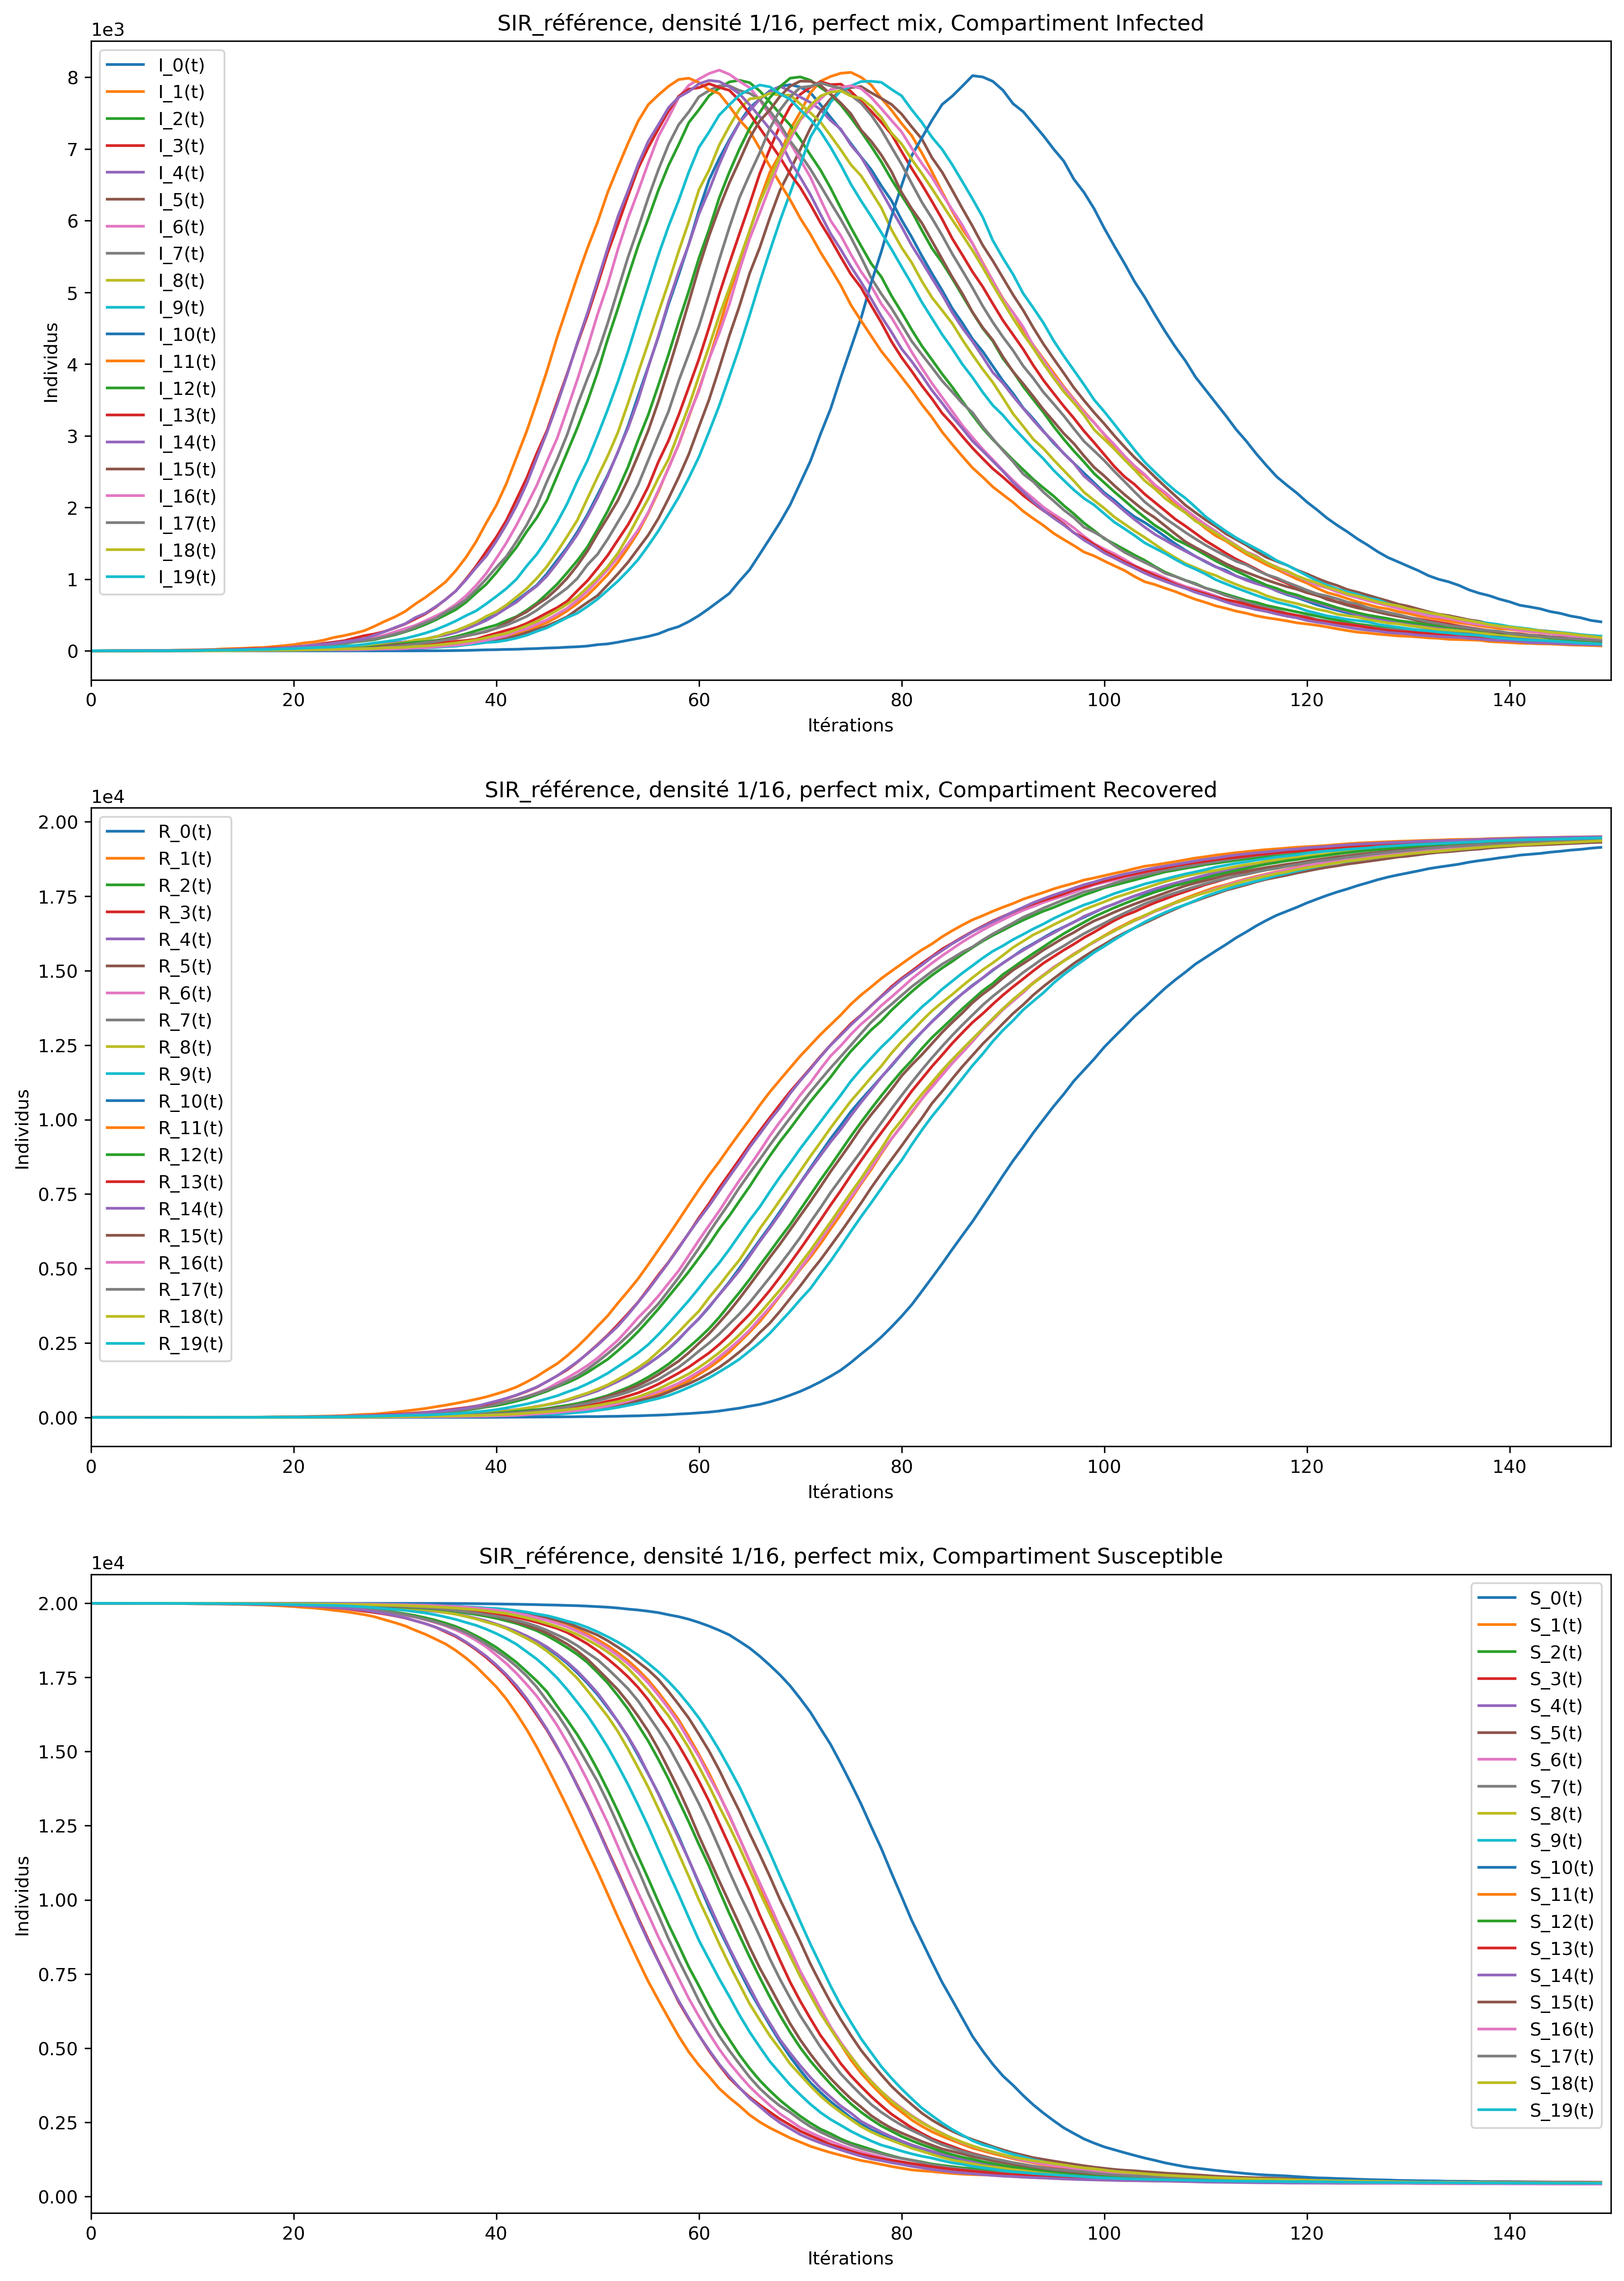
\includegraphics[width=0.5\textwidth]{Images/SIR_divergence_16_mix.png}
    \caption{Divergences SI}
\end{wrapfigure}

explications

\begin{table}[H]
	\centering
	\captionsetup{justification=centering}
	\caption[Variations : SIR]{Voisinage : modèle SIR\label{tab:grid}}
	\begin{tabular}{@{\extracolsep{\fill} } c|| c| c| c| c|}
	 & \multicolumn{2}{|c|}{1000 mouvements} & \multicolumn{2}{|c|}{Mélange parfait} \\
	\midrule
	\midrule
	densité & 1/8 & 1/16 & 1/8 & 1/16\\
	\midrule
	min & $24$ & $42$ & $22$ & $41$\\
	\midrule
	max & $32$ & $64$ & $37$ & $55$\\
	\midrule
	mean & $26.9$ & $50.15$ & $25.1$ & $47.7$\\
	\midrule
	std & $2.52$ & $5.81$ & $3.27$ & $4.63$\\
	\bottomrule
	\end{tabular}
	\end{table}

\subsection{Latence des simulations}

\subsection{Mouvements variable}

\begin{figure}[h]
	\centering
	\captionsetup{justification=centering}
	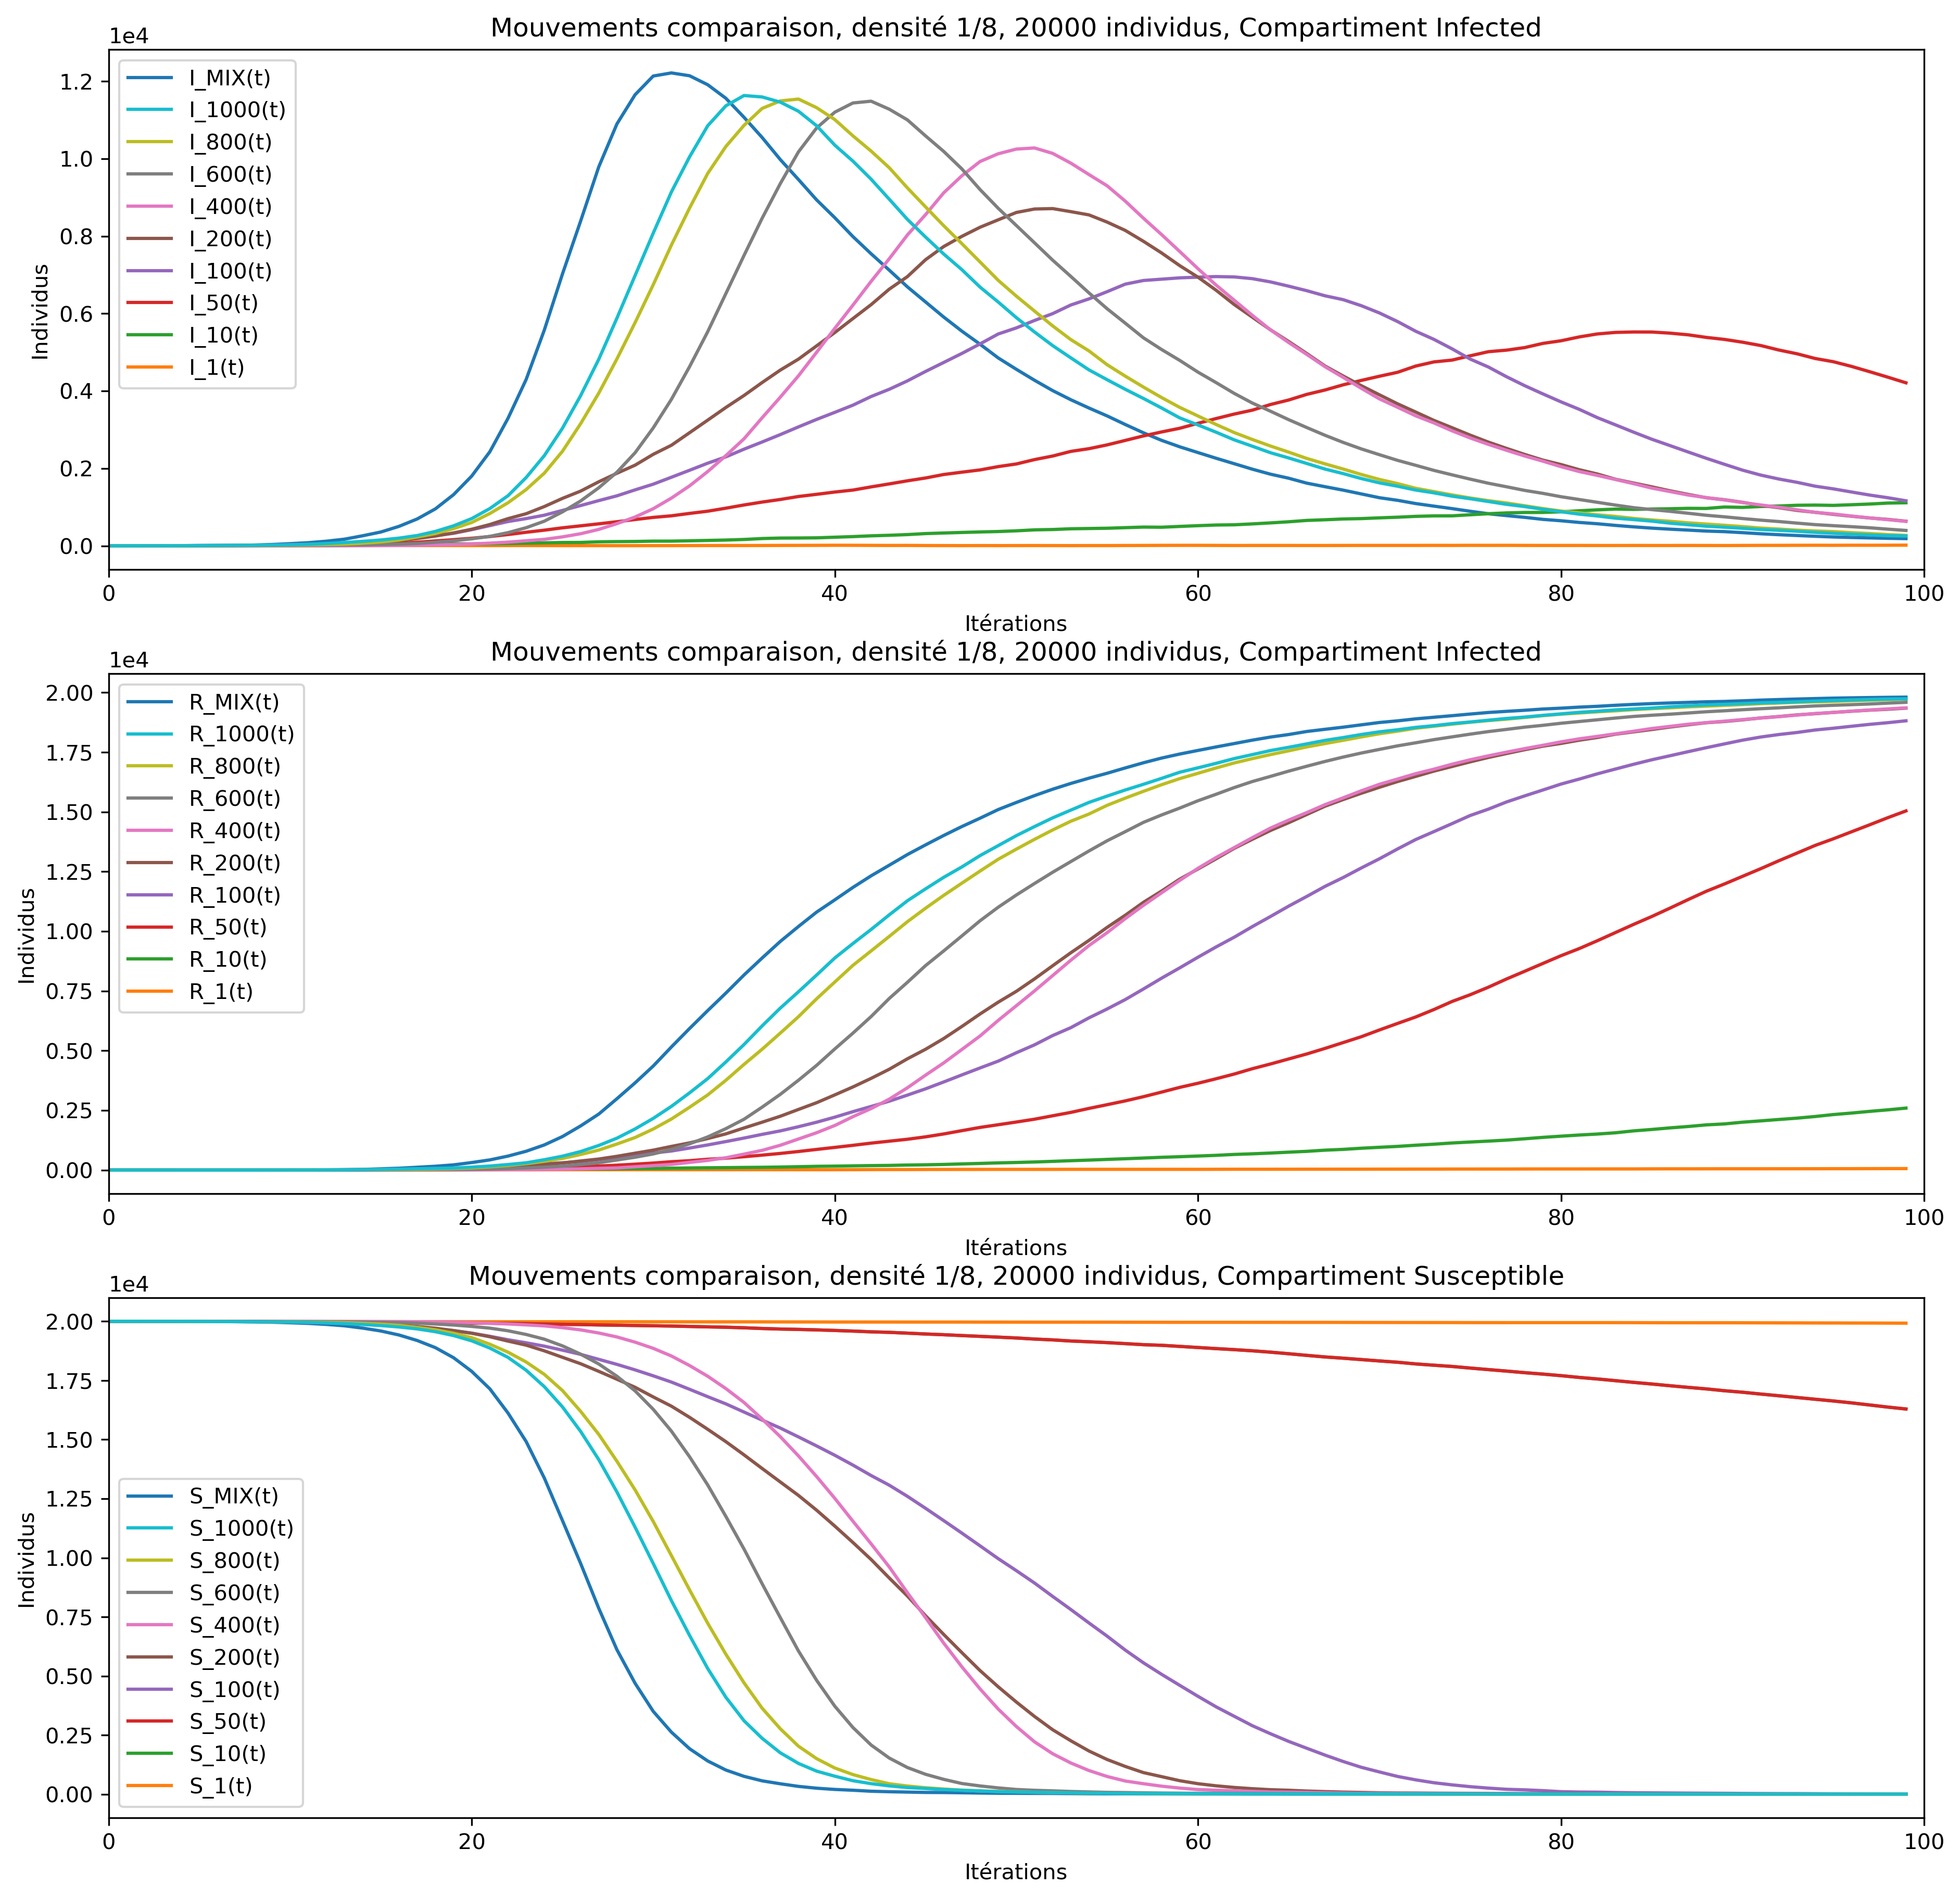
\includegraphics[width=.7\textwidth]{Images/SIR_mouvements_variables.png}
	\caption{test}
\end{figure}

\subsection{Comparaison 1000 mouvements}


